
% Default to the notebook output style

    


% Inherit from the specified cell style.




    
\documentclass[11pt]{article}

    
    
    \usepackage[T1]{fontenc}
    % Nicer default font (+ math font) than Computer Modern for most use cases
    \usepackage{mathpazo}

    % Basic figure setup, for now with no caption control since it's done
    % automatically by Pandoc (which extracts ![](path) syntax from Markdown).
    \usepackage{graphicx}
    % We will generate all images so they have a width \maxwidth. This means
    % that they will get their normal width if they fit onto the page, but
    % are scaled down if they would overflow the margins.
    \makeatletter
    \def\maxwidth{\ifdim\Gin@nat@width>\linewidth\linewidth
    \else\Gin@nat@width\fi}
    \makeatother
    \let\Oldincludegraphics\includegraphics
    % Set max figure width to be 80% of text width, for now hardcoded.
    \renewcommand{\includegraphics}[1]{\Oldincludegraphics[width=.8\maxwidth]{#1}}
    % Ensure that by default, figures have no caption (until we provide a
    % proper Figure object with a Caption API and a way to capture that
    % in the conversion process - todo).
    \usepackage{caption}
    \DeclareCaptionLabelFormat{nolabel}{}
    \captionsetup{labelformat=nolabel}

    \usepackage{adjustbox} % Used to constrain images to a maximum size 
    \usepackage{xcolor} % Allow colors to be defined
    \usepackage{enumerate} % Needed for markdown enumerations to work
    \usepackage{geometry} % Used to adjust the document margins
    \usepackage{amsmath} % Equations
    \usepackage{amssymb} % Equations
    \usepackage{textcomp} % defines textquotesingle
    % Hack from http://tex.stackexchange.com/a/47451/13684:
    \AtBeginDocument{%
        \def\PYZsq{\textquotesingle}% Upright quotes in Pygmentized code
    }
    \usepackage{upquote} % Upright quotes for verbatim code
    \usepackage{eurosym} % defines \euro
    \usepackage[mathletters]{ucs} % Extended unicode (utf-8) support
    \usepackage[utf8x]{inputenc} % Allow utf-8 characters in the tex document
    \usepackage{fancyvrb} % verbatim replacement that allows latex
    \usepackage{grffile} % extends the file name processing of package graphics 
                         % to support a larger range 
    % The hyperref package gives us a pdf with properly built
    % internal navigation ('pdf bookmarks' for the table of contents,
    % internal cross-reference links, web links for URLs, etc.)
    \usepackage{hyperref}
    \usepackage{longtable} % longtable support required by pandoc >1.10
    \usepackage{booktabs}  % table support for pandoc > 1.12.2
    \usepackage[inline]{enumitem} % IRkernel/repr support (it uses the enumerate* environment)
    \usepackage[normalem]{ulem} % ulem is needed to support strikethroughs (\sout)
                                % normalem makes italics be italics, not underlines
    

    
    
    % Colors for the hyperref package
    \definecolor{urlcolor}{rgb}{0,.145,.698}
    \definecolor{linkcolor}{rgb}{.71,0.21,0.01}
    \definecolor{citecolor}{rgb}{.12,.54,.11}

    % ANSI colors
    \definecolor{ansi-black}{HTML}{3E424D}
    \definecolor{ansi-black-intense}{HTML}{282C36}
    \definecolor{ansi-red}{HTML}{E75C58}
    \definecolor{ansi-red-intense}{HTML}{B22B31}
    \definecolor{ansi-green}{HTML}{00A250}
    \definecolor{ansi-green-intense}{HTML}{007427}
    \definecolor{ansi-yellow}{HTML}{DDB62B}
    \definecolor{ansi-yellow-intense}{HTML}{B27D12}
    \definecolor{ansi-blue}{HTML}{208FFB}
    \definecolor{ansi-blue-intense}{HTML}{0065CA}
    \definecolor{ansi-magenta}{HTML}{D160C4}
    \definecolor{ansi-magenta-intense}{HTML}{A03196}
    \definecolor{ansi-cyan}{HTML}{60C6C8}
    \definecolor{ansi-cyan-intense}{HTML}{258F8F}
    \definecolor{ansi-white}{HTML}{C5C1B4}
    \definecolor{ansi-white-intense}{HTML}{A1A6B2}

    % commands and environments needed by pandoc snippets
    % extracted from the output of `pandoc -s`
    \providecommand{\tightlist}{%
      \setlength{\itemsep}{0pt}\setlength{\parskip}{0pt}}
    \DefineVerbatimEnvironment{Highlighting}{Verbatim}{commandchars=\\\{\}}
    % Add ',fontsize=\small' for more characters per line
    \newenvironment{Shaded}{}{}
    \newcommand{\KeywordTok}[1]{\textcolor[rgb]{0.00,0.44,0.13}{\textbf{{#1}}}}
    \newcommand{\DataTypeTok}[1]{\textcolor[rgb]{0.56,0.13,0.00}{{#1}}}
    \newcommand{\DecValTok}[1]{\textcolor[rgb]{0.25,0.63,0.44}{{#1}}}
    \newcommand{\BaseNTok}[1]{\textcolor[rgb]{0.25,0.63,0.44}{{#1}}}
    \newcommand{\FloatTok}[1]{\textcolor[rgb]{0.25,0.63,0.44}{{#1}}}
    \newcommand{\CharTok}[1]{\textcolor[rgb]{0.25,0.44,0.63}{{#1}}}
    \newcommand{\StringTok}[1]{\textcolor[rgb]{0.25,0.44,0.63}{{#1}}}
    \newcommand{\CommentTok}[1]{\textcolor[rgb]{0.38,0.63,0.69}{\textit{{#1}}}}
    \newcommand{\OtherTok}[1]{\textcolor[rgb]{0.00,0.44,0.13}{{#1}}}
    \newcommand{\AlertTok}[1]{\textcolor[rgb]{1.00,0.00,0.00}{\textbf{{#1}}}}
    \newcommand{\FunctionTok}[1]{\textcolor[rgb]{0.02,0.16,0.49}{{#1}}}
    \newcommand{\RegionMarkerTok}[1]{{#1}}
    \newcommand{\ErrorTok}[1]{\textcolor[rgb]{1.00,0.00,0.00}{\textbf{{#1}}}}
    \newcommand{\NormalTok}[1]{{#1}}
    
    % Additional commands for more recent versions of Pandoc
    \newcommand{\ConstantTok}[1]{\textcolor[rgb]{0.53,0.00,0.00}{{#1}}}
    \newcommand{\SpecialCharTok}[1]{\textcolor[rgb]{0.25,0.44,0.63}{{#1}}}
    \newcommand{\VerbatimStringTok}[1]{\textcolor[rgb]{0.25,0.44,0.63}{{#1}}}
    \newcommand{\SpecialStringTok}[1]{\textcolor[rgb]{0.73,0.40,0.53}{{#1}}}
    \newcommand{\ImportTok}[1]{{#1}}
    \newcommand{\DocumentationTok}[1]{\textcolor[rgb]{0.73,0.13,0.13}{\textit{{#1}}}}
    \newcommand{\AnnotationTok}[1]{\textcolor[rgb]{0.38,0.63,0.69}{\textbf{\textit{{#1}}}}}
    \newcommand{\CommentVarTok}[1]{\textcolor[rgb]{0.38,0.63,0.69}{\textbf{\textit{{#1}}}}}
    \newcommand{\VariableTok}[1]{\textcolor[rgb]{0.10,0.09,0.49}{{#1}}}
    \newcommand{\ControlFlowTok}[1]{\textcolor[rgb]{0.00,0.44,0.13}{\textbf{{#1}}}}
    \newcommand{\OperatorTok}[1]{\textcolor[rgb]{0.40,0.40,0.40}{{#1}}}
    \newcommand{\BuiltInTok}[1]{{#1}}
    \newcommand{\ExtensionTok}[1]{{#1}}
    \newcommand{\PreprocessorTok}[1]{\textcolor[rgb]{0.74,0.48,0.00}{{#1}}}
    \newcommand{\AttributeTok}[1]{\textcolor[rgb]{0.49,0.56,0.16}{{#1}}}
    \newcommand{\InformationTok}[1]{\textcolor[rgb]{0.38,0.63,0.69}{\textbf{\textit{{#1}}}}}
    \newcommand{\WarningTok}[1]{\textcolor[rgb]{0.38,0.63,0.69}{\textbf{\textit{{#1}}}}}
    
    
    % Define a nice break command that doesn't care if a line doesn't already
    % exist.
    \def\br{\hspace*{\fill} \\* }
    % Math Jax compatability definitions
    \def\gt{>}
    \def\lt{<}
    % Document parameters
    \title{NNW - radial basis}
    
    
    

    % Pygments definitions
    
\makeatletter
\def\PY@reset{\let\PY@it=\relax \let\PY@bf=\relax%
    \let\PY@ul=\relax \let\PY@tc=\relax%
    \let\PY@bc=\relax \let\PY@ff=\relax}
\def\PY@tok#1{\csname PY@tok@#1\endcsname}
\def\PY@toks#1+{\ifx\relax#1\empty\else%
    \PY@tok{#1}\expandafter\PY@toks\fi}
\def\PY@do#1{\PY@bc{\PY@tc{\PY@ul{%
    \PY@it{\PY@bf{\PY@ff{#1}}}}}}}
\def\PY#1#2{\PY@reset\PY@toks#1+\relax+\PY@do{#2}}

\expandafter\def\csname PY@tok@w\endcsname{\def\PY@tc##1{\textcolor[rgb]{0.73,0.73,0.73}{##1}}}
\expandafter\def\csname PY@tok@c\endcsname{\let\PY@it=\textit\def\PY@tc##1{\textcolor[rgb]{0.25,0.50,0.50}{##1}}}
\expandafter\def\csname PY@tok@cp\endcsname{\def\PY@tc##1{\textcolor[rgb]{0.74,0.48,0.00}{##1}}}
\expandafter\def\csname PY@tok@k\endcsname{\let\PY@bf=\textbf\def\PY@tc##1{\textcolor[rgb]{0.00,0.50,0.00}{##1}}}
\expandafter\def\csname PY@tok@kp\endcsname{\def\PY@tc##1{\textcolor[rgb]{0.00,0.50,0.00}{##1}}}
\expandafter\def\csname PY@tok@kt\endcsname{\def\PY@tc##1{\textcolor[rgb]{0.69,0.00,0.25}{##1}}}
\expandafter\def\csname PY@tok@o\endcsname{\def\PY@tc##1{\textcolor[rgb]{0.40,0.40,0.40}{##1}}}
\expandafter\def\csname PY@tok@ow\endcsname{\let\PY@bf=\textbf\def\PY@tc##1{\textcolor[rgb]{0.67,0.13,1.00}{##1}}}
\expandafter\def\csname PY@tok@nb\endcsname{\def\PY@tc##1{\textcolor[rgb]{0.00,0.50,0.00}{##1}}}
\expandafter\def\csname PY@tok@nf\endcsname{\def\PY@tc##1{\textcolor[rgb]{0.00,0.00,1.00}{##1}}}
\expandafter\def\csname PY@tok@nc\endcsname{\let\PY@bf=\textbf\def\PY@tc##1{\textcolor[rgb]{0.00,0.00,1.00}{##1}}}
\expandafter\def\csname PY@tok@nn\endcsname{\let\PY@bf=\textbf\def\PY@tc##1{\textcolor[rgb]{0.00,0.00,1.00}{##1}}}
\expandafter\def\csname PY@tok@ne\endcsname{\let\PY@bf=\textbf\def\PY@tc##1{\textcolor[rgb]{0.82,0.25,0.23}{##1}}}
\expandafter\def\csname PY@tok@nv\endcsname{\def\PY@tc##1{\textcolor[rgb]{0.10,0.09,0.49}{##1}}}
\expandafter\def\csname PY@tok@no\endcsname{\def\PY@tc##1{\textcolor[rgb]{0.53,0.00,0.00}{##1}}}
\expandafter\def\csname PY@tok@nl\endcsname{\def\PY@tc##1{\textcolor[rgb]{0.63,0.63,0.00}{##1}}}
\expandafter\def\csname PY@tok@ni\endcsname{\let\PY@bf=\textbf\def\PY@tc##1{\textcolor[rgb]{0.60,0.60,0.60}{##1}}}
\expandafter\def\csname PY@tok@na\endcsname{\def\PY@tc##1{\textcolor[rgb]{0.49,0.56,0.16}{##1}}}
\expandafter\def\csname PY@tok@nt\endcsname{\let\PY@bf=\textbf\def\PY@tc##1{\textcolor[rgb]{0.00,0.50,0.00}{##1}}}
\expandafter\def\csname PY@tok@nd\endcsname{\def\PY@tc##1{\textcolor[rgb]{0.67,0.13,1.00}{##1}}}
\expandafter\def\csname PY@tok@s\endcsname{\def\PY@tc##1{\textcolor[rgb]{0.73,0.13,0.13}{##1}}}
\expandafter\def\csname PY@tok@sd\endcsname{\let\PY@it=\textit\def\PY@tc##1{\textcolor[rgb]{0.73,0.13,0.13}{##1}}}
\expandafter\def\csname PY@tok@si\endcsname{\let\PY@bf=\textbf\def\PY@tc##1{\textcolor[rgb]{0.73,0.40,0.53}{##1}}}
\expandafter\def\csname PY@tok@se\endcsname{\let\PY@bf=\textbf\def\PY@tc##1{\textcolor[rgb]{0.73,0.40,0.13}{##1}}}
\expandafter\def\csname PY@tok@sr\endcsname{\def\PY@tc##1{\textcolor[rgb]{0.73,0.40,0.53}{##1}}}
\expandafter\def\csname PY@tok@ss\endcsname{\def\PY@tc##1{\textcolor[rgb]{0.10,0.09,0.49}{##1}}}
\expandafter\def\csname PY@tok@sx\endcsname{\def\PY@tc##1{\textcolor[rgb]{0.00,0.50,0.00}{##1}}}
\expandafter\def\csname PY@tok@m\endcsname{\def\PY@tc##1{\textcolor[rgb]{0.40,0.40,0.40}{##1}}}
\expandafter\def\csname PY@tok@gh\endcsname{\let\PY@bf=\textbf\def\PY@tc##1{\textcolor[rgb]{0.00,0.00,0.50}{##1}}}
\expandafter\def\csname PY@tok@gu\endcsname{\let\PY@bf=\textbf\def\PY@tc##1{\textcolor[rgb]{0.50,0.00,0.50}{##1}}}
\expandafter\def\csname PY@tok@gd\endcsname{\def\PY@tc##1{\textcolor[rgb]{0.63,0.00,0.00}{##1}}}
\expandafter\def\csname PY@tok@gi\endcsname{\def\PY@tc##1{\textcolor[rgb]{0.00,0.63,0.00}{##1}}}
\expandafter\def\csname PY@tok@gr\endcsname{\def\PY@tc##1{\textcolor[rgb]{1.00,0.00,0.00}{##1}}}
\expandafter\def\csname PY@tok@ge\endcsname{\let\PY@it=\textit}
\expandafter\def\csname PY@tok@gs\endcsname{\let\PY@bf=\textbf}
\expandafter\def\csname PY@tok@gp\endcsname{\let\PY@bf=\textbf\def\PY@tc##1{\textcolor[rgb]{0.00,0.00,0.50}{##1}}}
\expandafter\def\csname PY@tok@go\endcsname{\def\PY@tc##1{\textcolor[rgb]{0.53,0.53,0.53}{##1}}}
\expandafter\def\csname PY@tok@gt\endcsname{\def\PY@tc##1{\textcolor[rgb]{0.00,0.27,0.87}{##1}}}
\expandafter\def\csname PY@tok@err\endcsname{\def\PY@bc##1{\setlength{\fboxsep}{0pt}\fcolorbox[rgb]{1.00,0.00,0.00}{1,1,1}{\strut ##1}}}
\expandafter\def\csname PY@tok@kc\endcsname{\let\PY@bf=\textbf\def\PY@tc##1{\textcolor[rgb]{0.00,0.50,0.00}{##1}}}
\expandafter\def\csname PY@tok@kd\endcsname{\let\PY@bf=\textbf\def\PY@tc##1{\textcolor[rgb]{0.00,0.50,0.00}{##1}}}
\expandafter\def\csname PY@tok@kn\endcsname{\let\PY@bf=\textbf\def\PY@tc##1{\textcolor[rgb]{0.00,0.50,0.00}{##1}}}
\expandafter\def\csname PY@tok@kr\endcsname{\let\PY@bf=\textbf\def\PY@tc##1{\textcolor[rgb]{0.00,0.50,0.00}{##1}}}
\expandafter\def\csname PY@tok@bp\endcsname{\def\PY@tc##1{\textcolor[rgb]{0.00,0.50,0.00}{##1}}}
\expandafter\def\csname PY@tok@fm\endcsname{\def\PY@tc##1{\textcolor[rgb]{0.00,0.00,1.00}{##1}}}
\expandafter\def\csname PY@tok@vc\endcsname{\def\PY@tc##1{\textcolor[rgb]{0.10,0.09,0.49}{##1}}}
\expandafter\def\csname PY@tok@vg\endcsname{\def\PY@tc##1{\textcolor[rgb]{0.10,0.09,0.49}{##1}}}
\expandafter\def\csname PY@tok@vi\endcsname{\def\PY@tc##1{\textcolor[rgb]{0.10,0.09,0.49}{##1}}}
\expandafter\def\csname PY@tok@vm\endcsname{\def\PY@tc##1{\textcolor[rgb]{0.10,0.09,0.49}{##1}}}
\expandafter\def\csname PY@tok@sa\endcsname{\def\PY@tc##1{\textcolor[rgb]{0.73,0.13,0.13}{##1}}}
\expandafter\def\csname PY@tok@sb\endcsname{\def\PY@tc##1{\textcolor[rgb]{0.73,0.13,0.13}{##1}}}
\expandafter\def\csname PY@tok@sc\endcsname{\def\PY@tc##1{\textcolor[rgb]{0.73,0.13,0.13}{##1}}}
\expandafter\def\csname PY@tok@dl\endcsname{\def\PY@tc##1{\textcolor[rgb]{0.73,0.13,0.13}{##1}}}
\expandafter\def\csname PY@tok@s2\endcsname{\def\PY@tc##1{\textcolor[rgb]{0.73,0.13,0.13}{##1}}}
\expandafter\def\csname PY@tok@sh\endcsname{\def\PY@tc##1{\textcolor[rgb]{0.73,0.13,0.13}{##1}}}
\expandafter\def\csname PY@tok@s1\endcsname{\def\PY@tc##1{\textcolor[rgb]{0.73,0.13,0.13}{##1}}}
\expandafter\def\csname PY@tok@mb\endcsname{\def\PY@tc##1{\textcolor[rgb]{0.40,0.40,0.40}{##1}}}
\expandafter\def\csname PY@tok@mf\endcsname{\def\PY@tc##1{\textcolor[rgb]{0.40,0.40,0.40}{##1}}}
\expandafter\def\csname PY@tok@mh\endcsname{\def\PY@tc##1{\textcolor[rgb]{0.40,0.40,0.40}{##1}}}
\expandafter\def\csname PY@tok@mi\endcsname{\def\PY@tc##1{\textcolor[rgb]{0.40,0.40,0.40}{##1}}}
\expandafter\def\csname PY@tok@il\endcsname{\def\PY@tc##1{\textcolor[rgb]{0.40,0.40,0.40}{##1}}}
\expandafter\def\csname PY@tok@mo\endcsname{\def\PY@tc##1{\textcolor[rgb]{0.40,0.40,0.40}{##1}}}
\expandafter\def\csname PY@tok@ch\endcsname{\let\PY@it=\textit\def\PY@tc##1{\textcolor[rgb]{0.25,0.50,0.50}{##1}}}
\expandafter\def\csname PY@tok@cm\endcsname{\let\PY@it=\textit\def\PY@tc##1{\textcolor[rgb]{0.25,0.50,0.50}{##1}}}
\expandafter\def\csname PY@tok@cpf\endcsname{\let\PY@it=\textit\def\PY@tc##1{\textcolor[rgb]{0.25,0.50,0.50}{##1}}}
\expandafter\def\csname PY@tok@c1\endcsname{\let\PY@it=\textit\def\PY@tc##1{\textcolor[rgb]{0.25,0.50,0.50}{##1}}}
\expandafter\def\csname PY@tok@cs\endcsname{\let\PY@it=\textit\def\PY@tc##1{\textcolor[rgb]{0.25,0.50,0.50}{##1}}}

\def\PYZbs{\char`\\}
\def\PYZus{\char`\_}
\def\PYZob{\char`\{}
\def\PYZcb{\char`\}}
\def\PYZca{\char`\^}
\def\PYZam{\char`\&}
\def\PYZlt{\char`\<}
\def\PYZgt{\char`\>}
\def\PYZsh{\char`\#}
\def\PYZpc{\char`\%}
\def\PYZdl{\char`\$}
\def\PYZhy{\char`\-}
\def\PYZsq{\char`\'}
\def\PYZdq{\char`\"}
\def\PYZti{\char`\~}
% for compatibility with earlier versions
\def\PYZat{@}
\def\PYZlb{[}
\def\PYZrb{]}
\makeatother


    % Exact colors from NB
    \definecolor{incolor}{rgb}{0.0, 0.0, 0.5}
    \definecolor{outcolor}{rgb}{0.545, 0.0, 0.0}



    
    % Prevent overflowing lines due to hard-to-break entities
    \sloppy 
    % Setup hyperref package
    \hypersetup{
      breaklinks=true,  % so long urls are correctly broken across lines
      colorlinks=true,
      urlcolor=urlcolor,
      linkcolor=linkcolor,
      citecolor=citecolor,
      }
    % Slightly bigger margins than the latex defaults
    
    \geometry{verbose,tmargin=1in,bmargin=1in,lmargin=1in,rmargin=1in}
    
    

    \begin{document}
    
    
    \maketitle
    
    

    
    \section{Import Required Packages}\label{import-required-packages}

    \begin{Verbatim}[commandchars=\\\{\}]
{\color{incolor}In [{\color{incolor}1}]:} \PY{k+kn}{import} \PY{n+nn}{numpy} \PY{k}{as} \PY{n+nn}{np}
        \PY{k+kn}{import} \PY{n+nn}{pandas} \PY{k}{as} \PY{n+nn}{pd}
        \PY{k+kn}{import} \PY{n+nn}{pygeostat} \PY{k}{as} \PY{n+nn}{gs}
        \PY{k+kn}{import} \PY{n+nn}{matplotlib}\PY{n+nn}{.}\PY{n+nn}{pyplot} \PY{k}{as} \PY{n+nn}{plt}
        \PY{k+kn}{import} \PY{n+nn}{matplotlib}\PY{n+nn}{.}\PY{n+nn}{cm} \PY{k}{as} \PY{n+nn}{cm}
        \PY{k+kn}{from} \PY{n+nn}{mpl\PYZus{}toolkits}\PY{n+nn}{.}\PY{n+nn}{axes\PYZus{}grid1} \PY{k}{import} \PY{n}{make\PYZus{}axes\PYZus{}locatable}
        \PY{k+kn}{import} \PY{n+nn}{subprocess} \PY{k}{as} \PY{n+nn}{sp}
        \PY{o}{\PYZpc{}}\PY{k}{pylab} inline \PYZhy{}\PYZhy{}no\PYZhy{}import\PYZhy{}all
        \PY{k+kn}{from} \PY{n+nn}{subprocess} \PY{k}{import} \PY{n}{check\PYZus{}output}
        \PY{k+kn}{import} \PY{n+nn}{tensorflow} \PY{k}{as} \PY{n+nn}{tf}
        \PY{k+kn}{from} \PY{n+nn}{tensorflow}\PY{n+nn}{.}\PY{n+nn}{python} \PY{k}{import} \PY{n}{debug} \PY{k}{as} \PY{n}{tf\PYZus{}debug}
        \PY{k+kn}{import} \PY{n+nn}{os}
        \PY{k+kn}{from} \PY{n+nn}{sklearn}\PY{n+nn}{.}\PY{n+nn}{preprocessing} \PY{k}{import} \PY{n}{MinMaxScaler}
        \PY{k+kn}{from} \PY{n+nn}{sklearn}\PY{n+nn}{.}\PY{n+nn}{model\PYZus{}selection} \PY{k}{import} \PY{n}{train\PYZus{}test\PYZus{}split}
        \PY{k+kn}{from} \PY{n+nn}{sklearn}\PY{n+nn}{.}\PY{n+nn}{preprocessing} \PY{k}{import} \PY{n}{LabelEncoder}
        \PY{k+kn}{from} \PY{n+nn}{sklearn}\PY{n+nn}{.}\PY{n+nn}{metrics} \PY{k}{import} \PY{n}{accuracy\PYZus{}score}
        \PY{k+kn}{from} \PY{n+nn}{sklearn}\PY{n+nn}{.}\PY{n+nn}{cluster} \PY{k}{import} \PY{n}{KMeans}
        \PY{k+kn}{from} \PY{n+nn}{sklearn} \PY{k}{import} \PY{n}{preprocessing}
        \PY{k+kn}{import} \PY{n+nn}{scipy}\PY{n+nn}{.}\PY{n+nn}{spatial} \PY{k}{as} \PY{n+nn}{scs}
        \PY{k+kn}{import} \PY{n+nn}{scipy} \PY{k}{as} \PY{n+nn}{sc}
        \PY{k+kn}{import} \PY{n+nn}{math}
        \PY{k+kn}{from} \PY{n+nn}{scipy}\PY{n+nn}{.}\PY{n+nn}{spatial} \PY{k}{import} \PY{n}{distance}
        \PY{k+kn}{from} \PY{n+nn}{sklearn}\PY{n+nn}{.}\PY{n+nn}{metrics} \PY{k}{import} \PY{n}{mean\PYZus{}squared\PYZus{}error}
        \PY{k+kn}{import} \PY{n+nn}{time}
        \PY{k+kn}{from} \PY{n+nn}{sklearn}\PY{n+nn}{.}\PY{n+nn}{metrics} \PY{k}{import} \PY{n}{r2\PYZus{}score}
        \PY{k+kn}{from} \PY{n+nn}{random} \PY{k}{import} \PY{n}{randrange}
        \PY{k+kn}{from} \PY{n+nn}{IPython}\PY{n+nn}{.}\PY{n+nn}{display} \PY{k}{import} \PY{n}{clear\PYZus{}output}
\end{Verbatim}


    \begin{Verbatim}[commandchars=\\\{\}]
Populating the interactive namespace from numpy and matplotlib

    \end{Verbatim}

    \begin{Verbatim}[commandchars=\\\{\}]
C:\textbackslash{}ProgramData\textbackslash{}Anaconda3\textbackslash{}lib\textbackslash{}site-packages\textbackslash{}h5py\textbackslash{}\_\_init\_\_.py:36: FutureWarning: Conversion of the second argument of issubdtype from `float` to `np.floating` is deprecated. In future, it will be treated as `np.float64 == np.dtype(float).type`.
  from .\_conv import register\_converters as \_register\_converters

    \end{Verbatim}

    \section{Import Grid Definition}\label{import-grid-definition}

    This is a 2D grid definition to keep the problem simple of illustration
purposes

    \begin{Verbatim}[commandchars=\\\{\}]
{\color{incolor}In [{\color{incolor}2}]:} \PY{n}{griddef} \PY{o}{=} \PY{n}{gs}\PY{o}{.}\PY{n}{GridDef}\PY{p}{(}\PY{n}{gridfl}\PY{o}{=}\PY{l+s+s1}{\PYZsq{}}\PY{l+s+s1}{griddef.txt}\PY{l+s+s1}{\PYZsq{}}\PY{p}{)}
        \PY{n}{griddef}
\end{Verbatim}


\begin{Verbatim}[commandchars=\\\{\}]
{\color{outcolor}Out[{\color{outcolor}2}]:} Pygeostat GridDef:
        50 5.0 10.0 
        50 5.0 10.0 
        1 0.5 1.0
\end{Verbatim}
            
    \section{Generate a Dataset}\label{generate-a-dataset}

    \subsection{Set Variogram Used To Simulate an Unconditional
Realization}\label{set-variogram-used-to-simulate-an-unconditional-realization}

    In this section we will be generating a sample data set used for machine
learning. The first step will be to define a variogram to use to
simulate an unconditional realization. Testing new techniques on
simulated data provides a unique opportunity to have a direct comparison
between the truth and the estimation.

    \begin{Verbatim}[commandchars=\\\{\}]
{\color{incolor}In [{\color{incolor}3}]:} \PY{n}{varg} \PY{o}{=} \PY{p}{(}\PY{l+s+s2}{\PYZdq{}}\PY{l+s+s2}{1    0.01                   \PYZhy{}nst, nugget effect}\PY{l+s+se}{\PYZbs{}n}\PY{l+s+se}{\PYZbs{}}
        \PY{l+s+s2}{3    0.99    135   45   0.0    \PYZhy{}it,cc,azm,dip,tilt (ang1,ang2,ang3)}\PY{l+s+se}{\PYZbs{}n}\PY{l+s+se}{\PYZbs{}}
        \PY{l+s+s2}{        100    100    150    \PYZhy{}a\PYZus{}hmax, a\PYZus{}hmin, a\PYZus{}vert (ranges)}\PY{l+s+s2}{\PYZdq{}}\PY{p}{)}
        
        \PY{n+nb}{print}\PY{p}{(}\PY{n}{varg}\PY{p}{)}
\end{Verbatim}


    \begin{Verbatim}[commandchars=\\\{\}]
1    0.01                   -nst, nugget effect
3    0.99    135   45   0.0    -it,cc,azm,dip,tilt (ang1,ang2,ang3)
        100    100    150    -a\_hmax, a\_hmin, a\_vert (ranges)

    \end{Verbatim}

    \subsection{Simulate Dataset}\label{simulate-dataset}

    In the cell below a 2D unconditional realization will be generated with
the variogram defined above

    \begin{Verbatim}[commandchars=\\\{\}]
{\color{incolor}In [{\color{incolor}4}]:} \PY{n}{sgsimpar} \PY{o}{=} \PY{l+s+s1}{\PYZsq{}\PYZsq{}\PYZsq{}}\PY{l+s+s1}{                  Parameters for SGSIM}
        \PY{l+s+s1}{                  ********************}
        
        \PY{l+s+s1}{START OF PARAMETERS:}
        \PY{l+s+s1}{cluster.dat           \PYZhy{}file with data}
        \PY{l+s+s1}{1  2  3  4  0  0              \PYZhy{}  columns for X,Y,Z,vr,wt,sec.var.}
        \PY{l+s+s1}{\PYZhy{}1.0       1.0e21             \PYZhy{}  trimming limits}
        \PY{l+s+s1}{0                             \PYZhy{}transform the data (0=no, 1=yes)}
        \PY{l+s+s1}{sgsim.trn                     \PYZhy{}  file for output trans table}
        \PY{l+s+s1}{0                             \PYZhy{}  consider ref. dist (0=no, 1=yes)}
        \PY{l+s+s1}{histsmth.out                  \PYZhy{}  file with ref. dist distribution}
        \PY{l+s+s1}{1  2                          \PYZhy{}  columns for vr and wt}
        \PY{l+s+s1}{0.0    15.0                   \PYZhy{}  zmin,zmax(tail extrapolation)}
        \PY{l+s+s1}{1       0.0                   \PYZhy{}  lower tail option, parameter}
        \PY{l+s+s1}{1      15.0                   \PYZhy{}  upper tail option, parameter}
        \PY{l+s+s1}{1                             \PYZhy{}debugging level: 0,1,2,3}
        \PY{l+s+s1}{sgsim.dbg                     \PYZhy{}file for debugging output}
        \PY{l+s+s1}{sgsim.out                     \PYZhy{}file for simulation output}
        \PY{l+s+s1}{1                             \PYZhy{}number of realizations to generate}
        \PY{l+s+si}{\PYZob{}grid\PYZcb{}}
        \PY{l+s+s1}{69069                         \PYZhy{}random number seed}
        \PY{l+s+s1}{0     8                       \PYZhy{}min and max original data for sim}
        \PY{l+s+s1}{48                            \PYZhy{}number of simulated nodes to use}
        \PY{l+s+s1}{1                             \PYZhy{}assign data to nodes (0=no, 1=yes)}
        \PY{l+s+s1}{1     3                       \PYZhy{}multiple grid search (0=no, 1=yes),num}
        \PY{l+s+s1}{0                             \PYZhy{}maximum data per octant (0=not used)}
        \PY{l+s+s1}{175  175.0  150.0              \PYZhy{}maximum search radii (hmax,hmin,vert)}
        \PY{l+s+s1}{135.0  45.0   0.0              \PYZhy{}angles for search ellipsoid}
        \PY{l+s+s1}{51    51    11                \PYZhy{}size of covariance lookup table}
        \PY{l+s+s1}{0     0.60   1.0              \PYZhy{}ktype: 0=SK,1=OK,2=LVM,3=EXDR,4=COLC}
        \PY{l+s+s1}{../data/ydata.dat             \PYZhy{}  file with LVM, EXDR, or COLC variable}
        \PY{l+s+s1}{4                             \PYZhy{}  column for secondary variable}
        \PY{l+s+si}{\PYZob{}varg\PYZcb{}}
        
        \PY{l+s+s1}{\PYZsq{}\PYZsq{}\PYZsq{}}
        \PY{n}{sgsim}\PY{o}{=} \PY{n}{gs}\PY{o}{.}\PY{n}{Program}\PY{p}{(}\PY{n}{program}\PY{o}{=}\PY{l+s+s1}{\PYZsq{}}\PY{l+s+s1}{sgsim}\PY{l+s+s1}{\PYZsq{}}\PY{p}{,}\PY{n}{parfile}\PY{o}{=}\PY{l+s+s1}{\PYZsq{}}\PY{l+s+s1}{sgsim.par}\PY{l+s+s1}{\PYZsq{}}\PY{p}{)}
        \PY{n}{sgsim}\PY{o}{.}\PY{n}{run}\PY{p}{(}\PY{n}{parstr}\PY{o}{=}\PY{n}{sgsimpar}\PY{o}{.}\PY{n}{format}\PY{p}{(}\PY{n}{varg} \PY{o}{=} \PY{n}{varg}\PY{p}{,}
                                         \PY{n}{grid} \PY{o}{=} \PY{n}{griddef}
                                        \PY{p}{)}\PY{p}{)}
\end{Verbatim}


    \begin{Verbatim}[commandchars=\\\{\}]
Calling:  ['sgsim', 'sgsim.par']

 SGSIM Version: 4.000

  data file = cluster.dat                             
  input columns =            1           2           3           4           0
           0
  trimming limits =   -1.000000      1.0000000E+21
  transformation flag =            0
  transformation file = sgsim.trn                               
  consider smoothed distribution (1=yes) =            0
  file with smoothed distribution = histsmth.out                            
  columns =            1           2
  data limits (tails) =   0.0000000E+00   15.00000    
  lower tail =            1  0.0000000E+00
  upper tail =            1   15.00000    
  debugging level =            1
  debugging file = sgsim.dbg                               
  output file sgsim.out                               
  number of realizations =            1
  X grid specification =           50   5.000000       10.00000    
  Y grid specification =           50   5.000000       10.00000    
  Z grid specification =            1  0.5000000       1.000000    
  random number seed =        69069
  min and max data =            0           8
  maximum previous nodes =           48
  two-part search flag =            1
  multiple grid search flag =            1           3
  number of octants =            0
  search radii =    175.0000       175.0000       150.0000    
  search anisotropy angles =    135.0000       45.00000      0.0000000E+00
  Automatically calculating max covariance table{\ldots}
  -  size needed for covariance lookup:    16   16    0
  kriging type =           51
 Old sgsim parameter file detected - reading again
  kriging type =            0
  secondary model file = ../data/ydata.dat                       
  column in secondary model file =            4
  nst, c0 =            1  9.9999998E-03
  it,cc,ang[1,2,3];            3  0.9900000       135.0000       45.00000    
  0.0000000E+00
  a1 a2 a3:    100.0000       100.0000       150.0000    
 
 WARNING data file 
 cluster.dat                                                                    
                                                                                
                                                                                
                                                                                
                                                                                
                                                                                
                                        does not exist!
    - Hope your intention was to create an unconditional simulation
    - Resetting ndmin, ndmax, and itrans  to 0 
    - Resetting sstrat to 1 
 Setting up rotation matrices for variogram and search
 
 Working on realization number            1
   currently on node       250
   currently on node       500
   currently on node       750
   currently on node      1000
   currently on node      1250
   currently on node      1500
   currently on node      1750
   currently on node      2000
   currently on node      2250
   currently on node      2500

 Realization   1: number   =     2500
                  mean     =       0.1086 (close to 0.0?)
                  variance =       0.8108 (close to gammabar(V,V)? approx. 1.0)


 SGSIM Version: 4.000 Finished


    \end{Verbatim}

    \subsubsection{Read in the Simulated
Dataset}\label{read-in-the-simulated-dataset}

    \begin{Verbatim}[commandchars=\\\{\}]
{\color{incolor}In [{\color{incolor}5}]:} \PY{n}{sgsimfl} \PY{o}{=} \PY{n}{gs}\PY{o}{.}\PY{n}{DataFile}\PY{p}{(}\PY{n}{flname}\PY{o}{=}\PY{l+s+s1}{\PYZsq{}}\PY{l+s+s1}{sgsim.out}\PY{l+s+s1}{\PYZsq{}}\PY{p}{,} \PY{n}{griddef} \PY{o}{=} \PY{n}{griddef}\PY{p}{,}
                               \PY{n}{readfl}\PY{o}{=}\PY{k+kc}{True}\PY{p}{)}
        \PY{n+nb}{print}\PY{p}{(}\PY{n}{sgsimfl}\PY{o}{.}\PY{n}{head}\PY{p}{(}\PY{p}{)}\PY{p}{)}
\end{Verbatim}


    \begin{Verbatim}[commandchars=\\\{\}]
      value
0 -1.514309
1 -1.496370
2 -1.095550
3 -1.116959
4 -0.983201

    \end{Verbatim}

    \subsubsection{Plot the Simulated
Dataset}\label{plot-the-simulated-dataset}

    \begin{Verbatim}[commandchars=\\\{\}]
{\color{incolor}In [{\color{incolor}6}]:} \PY{n}{gs}\PY{o}{.}\PY{n}{pixelplt}\PY{p}{(}\PY{n}{sgsimfl}\PY{p}{,}\PY{n}{griddef}\PY{p}{,}\PY{n}{orient}\PY{o}{=}\PY{l+s+s1}{\PYZsq{}}\PY{l+s+s1}{xy}\PY{l+s+s1}{\PYZsq{}}\PY{p}{)}
\end{Verbatim}


\begin{Verbatim}[commandchars=\\\{\}]
{\color{outcolor}Out[{\color{outcolor}6}]:} <mpl\_toolkits.axes\_grid1.axes\_divider.LocatableAxes at 0x1ffe5ec3c18>
\end{Verbatim}
            
    \begin{center}
    \adjustimage{max size={0.9\linewidth}{0.9\paperheight}}{output_15_1.png}
    \end{center}
    { \hspace*{\fill} \\}
    
    \subsection{Add coordinates to the Simulated Dataset to Be Used
Later}\label{add-coordinates-to-the-simulated-dataset-to-be-used-later}

    \begin{Verbatim}[commandchars=\\\{\}]
{\color{incolor}In [{\color{incolor}7}]:} \PY{n}{addcoordpar} \PY{o}{=} \PY{l+s+s1}{\PYZsq{}\PYZsq{}\PYZsq{}}\PY{l+s+s1}{                  Parameters for ADDCOORD}
        \PY{l+s+s1}{                  ***********************}
        
        \PY{l+s+s1}{START OF PARAMETERS:}
        \PY{l+s+si}{\PYZob{}datafl\PYZcb{}}\PY{l+s+s1}{                         \PYZhy{}file with data}
        \PY{l+s+s1}{addcoord.out                      \PYZhy{}file for output}
        \PY{l+s+s1}{1                                 \PYZhy{}realization number}
        \PY{l+s+si}{\PYZob{}grid\PYZcb{}}
        \PY{l+s+s1}{3 3 6                            \PYZhy{}decimals for x, y, z (\PYZhy{}1=exclude)}
        \PY{l+s+s1}{\PYZsq{}\PYZsq{}\PYZsq{}}
        \PY{n}{addcoord}\PY{o}{=} \PY{n}{gs}\PY{o}{.}\PY{n}{Program}\PY{p}{(}\PY{n}{program}\PY{o}{=}\PY{l+s+s1}{\PYZsq{}}\PY{l+s+s1}{addcoord}\PY{l+s+s1}{\PYZsq{}}\PY{p}{,}\PY{n}{parfile}\PY{o}{=}\PY{l+s+s1}{\PYZsq{}}\PY{l+s+s1}{addcoord.par}\PY{l+s+s1}{\PYZsq{}}\PY{p}{)}
        \PY{n}{addcoord}\PY{o}{.}\PY{n}{run}\PY{p}{(}\PY{n}{parstr}\PY{o}{=}\PY{n}{addcoordpar}\PY{o}{.}\PY{n}{format}\PY{p}{(}\PY{n}{datafl}\PY{o}{=}\PY{n}{sgsimfl}\PY{o}{.}\PY{n}{flname}
                                        \PY{p}{,}\PY{n}{grid} \PY{o}{=} \PY{n}{griddef}
                                        \PY{p}{)}\PY{p}{)}
\end{Verbatim}


    \begin{Verbatim}[commandchars=\\\{\}]
Calling:  ['addcoord', 'addcoord.par']

 ADDCOORD VERSION: 4.1.0

 Data File = sgsim.out                               
 Output File = addcoord.out                            
 Realization number =            1
 X grid size =           50   5.00000000000000        10.0000000000000     
 Y grid size =           50   5.00000000000000        10.0000000000000     
 Z grid size =            1  0.500000000000000        1.00000000000000     
 decimals =            3           3           6
 
 Format: (f07.03,x,f07.03,x,f07.06,x,a)      

 ADDCOORD: 4.1.0 Finished


    \end{Verbatim}

    \subsubsection{Read in Simulation with
Coordinates}\label{read-in-simulation-with-coordinates}

    \begin{Verbatim}[commandchars=\\\{\}]
{\color{incolor}In [{\color{incolor}8}]:} \PY{n}{datafl} \PY{o}{=} \PY{n}{gs}\PY{o}{.}\PY{n}{DataFile}\PY{p}{(}\PY{n}{flname} \PY{o}{=} \PY{l+s+s1}{\PYZsq{}}\PY{l+s+s1}{addcoord.out}\PY{l+s+s1}{\PYZsq{}}\PY{p}{,}\PY{n}{x}\PY{o}{=}\PY{l+s+s1}{\PYZsq{}}\PY{l+s+s1}{X}\PY{l+s+s1}{\PYZsq{}}\PY{p}{,}\PY{n}{y}\PY{o}{=}\PY{l+s+s1}{\PYZsq{}}\PY{l+s+s1}{Y}\PY{l+s+s1}{\PYZsq{}}\PY{p}{,}\PY{n}{z}\PY{o}{=}\PY{l+s+s1}{\PYZsq{}}\PY{l+s+s1}{Z}\PY{l+s+s1}{\PYZsq{}}\PY{p}{,} \PY{n}{griddef}\PY{o}{=}\PY{n}{griddef}\PY{p}{,}
        \PY{n}{readfl}\PY{o}{=}\PY{k+kc}{True}\PY{p}{)}
        \PY{n+nb}{print}\PY{p}{(}\PY{n}{datafl}\PY{o}{.}\PY{n}{data}\PY{o}{.}\PY{n}{head}\PY{p}{(}\PY{p}{)}\PY{p}{)}
\end{Verbatim}


    \begin{Verbatim}[commandchars=\\\{\}]
      X    Y    Z     value
0   5.0  5.0  0.5 -1.514309
1  15.0  5.0  0.5 -1.496370
2  25.0  5.0  0.5 -1.095550
3  35.0  5.0  0.5 -1.116959
4  45.0  5.0  0.5 -0.983201

    \end{Verbatim}

    I like to re-plot the simulated data to help ensure nothing weird has
gone on

    \begin{Verbatim}[commandchars=\\\{\}]
{\color{incolor}In [{\color{incolor}9}]:} \PY{n}{gs}\PY{o}{.}\PY{n}{pixelplt}\PY{p}{(}\PY{n}{sgsimfl}\PY{p}{,}\PY{n}{griddef}\PY{p}{,}\PY{n}{title} \PY{o}{=} \PY{l+s+s1}{\PYZsq{}}\PY{l+s+s1}{truth}\PY{l+s+s1}{\PYZsq{}}\PY{p}{,}\PY{n}{vlim} \PY{o}{=} \PY{p}{(}\PY{o}{\PYZhy{}}\PY{l+m+mf}{1.5}\PY{p}{,}\PY{l+m+mf}{1.5}\PY{p}{)}\PY{p}{)}
\end{Verbatim}


\begin{Verbatim}[commandchars=\\\{\}]
{\color{outcolor}Out[{\color{outcolor}9}]:} <mpl\_toolkits.axes\_grid1.axes\_divider.LocatableAxes at 0x1ffe5a0ff98>
\end{Verbatim}
            
    \begin{center}
    \adjustimage{max size={0.9\linewidth}{0.9\paperheight}}{output_21_1.png}
    \end{center}
    { \hspace*{\fill} \\}
    
    \subsection{Sample The Simulated
Drill}\label{sample-the-simulated-drill}

    The program below is designed to sample a gridded data set either by
drill holes spacing or randomly sample the grid

    \begin{Verbatim}[commandchars=\\\{\}]
{\color{incolor}In [{\color{incolor}10}]:} \PY{n}{gsamplepar} \PY{o}{=} \PY{l+s+s1}{\PYZsq{}\PYZsq{}\PYZsq{}}\PY{l+s+s1}{       Parameters for gsample V2.000}
         \PY{l+s+s1}{     *********************************}
         \PY{l+s+s1}{       }
         \PY{l+s+s1}{START OF PARAMETERS:}
         \PY{l+s+s1}{1                            \PYZhy{} Number of files to sample}
         \PY{l+s+si}{\PYZob{}datafl\PYZcb{}}\PY{l+s+s1}{            \PYZhy{} File with first grid}
         \PY{l+s+s1}{1  }\PY{l+s+si}{\PYZob{}varcol1\PYZcb{}}\PY{l+s+s1}{                        \PYZhy{} Number of variables and columns}
         \PY{l+s+s1}{1                            \PYZhy{} Realization to sample}
         \PY{l+s+si}{\PYZob{}griddef\PYZcb{}}
         \PY{l+s+s1}{0                            \PYZhy{} Sampling spacing option (0=regular, 1=random)}
         \PY{l+s+s1}{25  25                       \PYZhy{}  If 0, spacing in X, Y}
         \PY{l+s+s1}{20  20                     \PYZhy{}  If 0, collar of the first sample, X and Y (inside sampling grid)}
         \PY{l+s+s1}{80  69069                    \PYZhy{}  If 1, number of drill holes and seed number}
         \PY{l+s+s1}{0  90                        \PYZhy{} Azimuth and dip}
         \PY{l+s+s1}{0.5                            \PYZhy{} Sample spacing downhole}
         \PY{l+s+s1}{1                          \PYZhy{} Starting drill hole ID for new drills}
         \PY{l+s+s1}{2                            \PYZhy{} Number of decimal places (coordinates precision, up to 6)}
         \PY{l+s+s1}{0   495                       \PYZhy{} Sampling grid: xmin, xmax}
         \PY{l+s+s1}{0   495                       \PYZhy{}                ymin, ymax}
         \PY{l+s+s1}{0   1                       \PYZhy{}                zmin, zmax}
         \PY{l+s+s1}{dhs.out        \PYZhy{} Output file with new drill holes}
         \PY{l+s+s1}{0                            \PYZhy{} Output keyout file? (0=no, 1=yes)}
         \PY{l+s+s1}{0                            \PYZhy{}  If keyout (0=input grid inside sampling grid, 1=input blocks with assays)}
         \PY{l+s+s1}{keyout.out         \PYZhy{} Keyout file}
         \PY{l+s+s1}{\PYZsq{}\PYZsq{}\PYZsq{}}
         \PY{n}{gsample}\PY{o}{=} \PY{n}{gs}\PY{o}{.}\PY{n}{Program}\PY{p}{(}\PY{n}{program}\PY{o}{=}\PY{l+s+s1}{\PYZsq{}}\PY{l+s+s1}{gsample}\PY{l+s+s1}{\PYZsq{}}\PY{p}{,}\PY{n}{parfile}\PY{o}{=}\PY{l+s+s1}{\PYZsq{}}\PY{l+s+s1}{gsample.par}\PY{l+s+s1}{\PYZsq{}}\PY{p}{)}
         \PY{n}{gsample}\PY{o}{.}\PY{n}{run}\PY{p}{(}\PY{n}{parstr}\PY{o}{=}\PY{n}{gsamplepar}\PY{o}{.}\PY{n}{format}\PY{p}{(}\PY{n}{datafl}\PY{o}{=}\PY{n}{datafl}\PY{o}{.}\PY{n}{flname}\PY{p}{,}
                                                \PY{n}{varcol1}\PY{o}{=}\PY{n}{datafl}\PY{o}{.}\PY{n}{gscol}\PY{p}{(}\PY{l+s+s1}{\PYZsq{}}\PY{l+s+s1}{value}\PY{l+s+s1}{\PYZsq{}}\PY{p}{)}\PY{p}{,}
                                                  \PY{n}{griddef}\PY{o}{=}\PY{n}{griddef}
                                               \PY{p}{)}\PY{p}{)}
\end{Verbatim}


    \begin{Verbatim}[commandchars=\\\{\}]
Calling:  ['gsample', 'gsample.par']

GSAMPLE Version: 1.000

PARAMETER FILE                  = gsample.par                                                                                                                                                                                                                                                     
-----------------------------------------------------------------------------

INPUT PARAMETERS 

Number of grids to sample       =   1
Total number of variables       =   1
 
Data file  1                    = 
addcoord.out
Variable columns                =   4
 
Sample realization number       =   1
 
Input grid 
Input grid in X                 =   50        5.00   10.00
Input grid in Y                 =   50        5.00   10.00
Input grid in Z                 =    1        0.50    1.00
 
Sample option                   =   0
 
Consider regular spacing 

 
Spacing in X                    =    25.0    
Spacing in Y                    =    25.0    
 
Collar in X                     =    20.0    
Collar in Y                     =    20.0    
 
Azimuth                         =    0.00    
Dip                             =    90.0    
 
Sample distance downhole        =   0.500    
 
Starting new drills with ID     =      1
 
Number of decimal places        = 2
 
Sampling grid 
 
Minimum and maximum in X        =        0.00      495.00
Minimum and maximum in Y        =        0.00      495.00
Minimum and maximum in Z        =        0.00        1.00
 
-----------------------------------------------------------------------------

OUTPUT PARAMETERS 

 
OUTPUT FILE                     = dhs.out                                                     
 
Do not output keyout array


-----------------------------------------------------------------------------

READING DATA

PREPARING OUTPUT FILES

-----------------------------------------------------------------------------

Allocating memory 

Finding block indices 

Sampling from grid 

Number of drill holes successfully created =  361
-----------------------------------------------------------------------------

END

Total execution time 0.020 seconds.

    \end{Verbatim}

    \subsubsection{Import the Sampled Drill
Holes}\label{import-the-sampled-drill-holes}

    \begin{Verbatim}[commandchars=\\\{\}]
{\color{incolor}In [{\color{incolor}11}]:} \PY{n}{dataflpoints} \PY{o}{=} \PY{n}{gs}\PY{o}{.}\PY{n}{DataFile}\PY{p}{(}\PY{n}{flname}\PY{o}{=}\PY{l+s+s1}{\PYZsq{}}\PY{l+s+s1}{dhs.out}\PY{l+s+s1}{\PYZsq{}}\PY{p}{,} \PY{n}{x}\PY{o}{=}\PY{l+s+s1}{\PYZsq{}}\PY{l+s+s1}{X}\PY{l+s+s1}{\PYZsq{}}\PY{p}{,}\PY{n}{y}\PY{o}{=}\PY{l+s+s1}{\PYZsq{}}\PY{l+s+s1}{Y}\PY{l+s+s1}{\PYZsq{}}\PY{p}{,}\PY{n}{z}\PY{o}{=}\PY{l+s+s1}{\PYZsq{}}\PY{l+s+s1}{Z}\PY{l+s+s1}{\PYZsq{}}\PY{p}{,} \PY{n}{griddef} \PY{o}{=} \PY{n}{griddef}\PY{p}{,}
                                \PY{n}{readfl}\PY{o}{=}\PY{k+kc}{True}\PY{p}{)}
         \PY{n}{dataflpoints}\PY{o}{.}\PY{n}{describe}\PY{p}{(}\PY{p}{)}
\end{Verbatim}


\begin{Verbatim}[commandchars=\\\{\}]
{\color{outcolor}Out[{\color{outcolor}11}]:}          Drill ID          MD     Block ID       value
         count  722.000000  722.000000   722.000000  722.000000
         mean   181.000000    0.250000  1238.421053    0.136465
         std    104.283567    0.250173   685.378723    0.871761
         min      1.000000    0.000000   103.000000   -1.931300
         25\%     91.000000    0.000000   638.000000   -0.427700
         50\%    181.000000    0.250000  1225.000000    0.068100
         75\%    271.000000    0.500000  1863.000000    0.601800
         max    361.000000    0.500000  2398.000000    2.911800
\end{Verbatim}
            
    Again it is useful to plot the drill holes and see what they look like

    \begin{Verbatim}[commandchars=\\\{\}]
{\color{incolor}In [{\color{incolor}12}]:} \PY{n}{gs}\PY{o}{.}\PY{n}{locmap}\PY{p}{(}\PY{n}{dataflpoints}\PY{p}{,}\PY{n}{var} \PY{o}{=} \PY{l+s+s1}{\PYZsq{}}\PY{l+s+s1}{value}\PY{l+s+s1}{\PYZsq{}}\PY{p}{,}\PY{n}{orient}\PY{o}{=}\PY{l+s+s1}{\PYZsq{}}\PY{l+s+s1}{xy}\PY{l+s+s1}{\PYZsq{}}\PY{p}{)}
\end{Verbatim}


\begin{Verbatim}[commandchars=\\\{\}]
{\color{outcolor}Out[{\color{outcolor}12}]:} <mpl\_toolkits.axes\_grid1.axes\_divider.LocatableAxes at 0x1ffe8123b38>
\end{Verbatim}
            
    \begin{center}
    \adjustimage{max size={0.9\linewidth}{0.9\paperheight}}{output_28_1.png}
    \end{center}
    { \hspace*{\fill} \\}
    
    \begin{Verbatim}[commandchars=\\\{\}]
{\color{incolor}In [{\color{incolor}13}]:} \PY{n+nb}{print}\PY{p}{(}\PY{l+s+s1}{\PYZsq{}}\PY{l+s+s1}{Here I am removing columns that are not necessary to make the data set easier to work with}\PY{l+s+s1}{\PYZsq{}}\PY{p}{)}
         \PY{n}{datasamplefl} \PY{o}{=} \PY{n}{pd}\PY{o}{.}\PY{n}{DataFrame}\PY{p}{(}\PY{n}{dataflpoints}\PY{o}{.}\PY{n}{data}\PY{p}{,} \PY{n}{dtype} \PY{o}{=} \PY{n}{np}\PY{o}{.}\PY{n}{float32}\PY{p}{)}
         \PY{k}{del} \PY{n}{datasamplefl}\PY{p}{[}\PY{l+s+s1}{\PYZsq{}}\PY{l+s+s1}{Drill ID}\PY{l+s+s1}{\PYZsq{}}\PY{p}{]}
         \PY{k}{del} \PY{n}{datasamplefl}\PY{p}{[}\PY{l+s+s1}{\PYZsq{}}\PY{l+s+s1}{MD}\PY{l+s+s1}{\PYZsq{}}\PY{p}{]}
         \PY{k}{del} \PY{n}{datasamplefl}\PY{p}{[}\PY{l+s+s1}{\PYZsq{}}\PY{l+s+s1}{Block ID}\PY{l+s+s1}{\PYZsq{}}\PY{p}{]}
         \PY{n}{datasamplefl}\PY{p}{[}\PY{l+s+s1}{\PYZsq{}}\PY{l+s+s1}{Z}\PY{l+s+s1}{\PYZsq{}}\PY{p}{]} \PY{o}{=} \PY{n}{datasamplefl}\PY{p}{[}\PY{l+s+s1}{\PYZsq{}}\PY{l+s+s1}{Z}\PY{l+s+s1}{\PYZsq{}}\PY{p}{]}
         \PY{n}{datasamplefl}\PY{o}{.}\PY{n}{drop\PYZus{}duplicates}\PY{p}{(}\PY{l+s+s1}{\PYZsq{}}\PY{l+s+s1}{value}\PY{l+s+s1}{\PYZsq{}}\PY{p}{)}
\end{Verbatim}


    \begin{Verbatim}[commandchars=\\\{\}]
Here I am removing columns that are not necessary to make the data set easier to work with

    \end{Verbatim}

\begin{Verbatim}[commandchars=\\\{\}]
{\color{outcolor}Out[{\color{outcolor}13}]:}          X      Y    Z   value
         0     20.0   20.0  1.0 -1.4885
         2     45.0   20.0  1.0 -1.2157
         4     70.0   20.0  1.0 -0.3973
         6     95.0   20.0  1.0  0.3458
         8    120.0   20.0  1.0  0.8231
         10   145.0   20.0  1.0  0.6026
         12   170.0   20.0  1.0 -0.1281
         14   195.0   20.0  1.0 -0.1794
         16   220.0   20.0  1.0  0.3482
         18   245.0   20.0  1.0  0.3846
         20   270.0   20.0  1.0 -0.0652
         22   295.0   20.0  1.0 -0.9595
         24   320.0   20.0  1.0 -1.2509
         26   345.0   20.0  1.0 -0.0172
         28   370.0   20.0  1.0  2.2261
         30   395.0   20.0  1.0  2.9118
         32   420.0   20.0  1.0  1.2570
         34   445.0   20.0  1.0 -0.6249
         36   470.0   20.0  1.0 -1.3088
         38    20.0   45.0  1.0 -1.5736
         40    45.0   45.0  1.0 -1.2523
         42    70.0   45.0  1.0 -0.1830
         44    95.0   45.0  1.0  0.2923
         46   120.0   45.0  1.0  0.7342
         48   145.0   45.0  1.0  0.7782
         50   170.0   45.0  1.0 -0.2147
         52   195.0   45.0  1.0  0.1865
         54   220.0   45.0  1.0  0.4281
         56   245.0   45.0  1.0  0.6109
         58   270.0   45.0  1.0 -0.4787
         ..     {\ldots}    {\ldots}  {\ldots}     {\ldots}
         662  220.0  445.0  1.0  0.4360
         664  245.0  445.0  1.0  0.0584
         666  270.0  445.0  1.0  0.0026
         668  295.0  445.0  1.0 -0.3673
         670  320.0  445.0  1.0 -0.5285
         672  345.0  445.0  1.0 -0.4795
         674  370.0  445.0  1.0 -0.5237
         676  395.0  445.0  1.0 -0.0986
         678  420.0  445.0  1.0  0.8788
         680  445.0  445.0  1.0  1.3183
         682  470.0  445.0  1.0  1.6706
         684   20.0  470.0  1.0 -1.1175
         686   45.0  470.0  1.0 -1.3712
         688   70.0  470.0  1.0 -1.7002
         690   95.0  470.0  1.0 -1.0341
         692  120.0  470.0  1.0  0.3926
         694  145.0  470.0  1.0  0.9616
         696  170.0  470.0  1.0  0.4342
         698  195.0  470.0  1.0  0.3131
         700  220.0  470.0  1.0  0.1116
         702  245.0  470.0  1.0 -0.2384
         704  270.0  470.0  1.0 -0.9453
         706  295.0  470.0  1.0 -1.1373
         708  320.0  470.0  1.0 -1.1996
         710  345.0  470.0  1.0 -1.5140
         712  370.0  470.0  1.0 -1.7595
         714  395.0  470.0  1.0 -0.9943
         716  420.0  470.0  1.0  0.4491
         718  445.0  470.0  1.0  1.4270
         720  470.0  470.0  1.0  1.7631
         
         [356 rows x 4 columns]
\end{Verbatim}
            
    \begin{Verbatim}[commandchars=\\\{\}]
{\color{incolor}In [{\color{incolor}14}]:} \PY{n}{datasamplefl} \PY{o}{=} \PY{n}{datasamplefl}\PY{p}{[}\PY{n}{pd}\PY{o}{.}\PY{n}{notnull}\PY{p}{(}\PY{n}{datasamplefl}\PY{p}{[}\PY{l+s+s1}{\PYZsq{}}\PY{l+s+s1}{value}\PY{l+s+s1}{\PYZsq{}}\PY{p}{]}\PY{p}{)}\PY{p}{]}
         \PY{n}{datasamplefl}\PY{o}{.}\PY{n}{describe}\PY{p}{(}\PY{p}{)}
\end{Verbatim}


\begin{Verbatim}[commandchars=\\\{\}]
{\color{outcolor}Out[{\color{outcolor}14}]:}                 X           Y           Z       value
         count  722.000000  722.000000  722.000000  722.000000
         mean   245.000000  245.000000    0.750000    0.136464
         std    137.025574  137.025574    0.250173    0.871761
         min     20.000000   20.000000    0.500000   -1.931300
         25\%    120.000000  120.000000    0.500000   -0.427700
         50\%    245.000000  245.000000    0.750000    0.068100
         75\%    370.000000  370.000000    1.000000    0.601800
         max    470.000000  470.000000    1.000000    2.911800
\end{Verbatim}
            
    \begin{Verbatim}[commandchars=\\\{\}]
{\color{incolor}In [{\color{incolor}15}]:} \PY{n}{gs}\PY{o}{.}\PY{n}{write\PYZus{}gslib}\PY{p}{(}\PY{n}{datasamplefl}\PY{p}{,} \PY{l+s+s1}{\PYZsq{}}\PY{l+s+s1}{datasamplefl.out}\PY{l+s+s1}{\PYZsq{}}\PY{p}{)}
\end{Verbatim}


    \begin{Verbatim}[commandchars=\\\{\}]
{\color{incolor}In [{\color{incolor}16}]:} \PY{n}{datatest} \PY{o}{=} \PY{n}{np}\PY{o}{.}\PY{n}{asarray}\PY{p}{(}\PY{n}{datasamplefl}\PY{p}{)}
\end{Verbatim}


    \section{Machine Learning}\label{machine-learning}

    \subsection{Types of Machine Learning}\label{types-of-machine-learning}

    ML is typically divided into two categories: supervised learning,
unsupervised learning, and some times, semi-supervised. Both supervised,
and unsupervised learning methods follow a similar three-step process of
training, testing, and application, as seen in the figure below. In
supervised learning, the ML algorithm has input features \(x_s\) which
are then used to predict the solution \(y_s\), during training the
solution to the hypothesis is known and used to generate/test the ML
algorithm which is why the process is known as supervised learning.
After the ML algorithm is trained and the hypothesis is validated using
k-fold validation or cross-validation the ML algorithm can be used to
predict/classify similar problems with the same input features \(x_s\)
where the solution \(y_s\) is not know. Different types of supervised
learning techniques include but are not limited to regression, decision
trees, random forests, support vector machines, and neural networks. For
the purposes of this thesis, the key supervised ML methods that will be
explored will be neural networks.

\begin{figure}[htbp!] % Data Storage
        \centering
        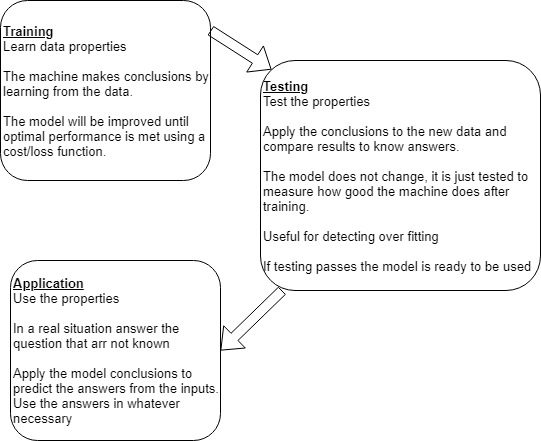
\includegraphics[width=1\linewidth]{figures/MLStages-1-638x467.png}
        \caption{Stages in Machine Learning}
        \label{fig:Stages In Machine Learning}
    \end{figure}

    In unsupervised learning the ML algorithm has input features \(x_s\)
which are then used to predict the solution \(y_s\), however; during
training the ML algorithm the answer to the hypothesis \(y_s\) is not
known. Again the solution to the hypothesis will need to be verified by
using k-fold validation, cross-validation, or by minimizing error in
dimension reduction techniques. Unsupervised learning techniques include
but are not limited to k-mean clustering, principal component analysis,
and reinforcement learning. For the purposes of this thesis, the primary
unsupervised ML method that will be explored will be k-means clustering.
A brief example of supervised vs. unsupervised machine learning
techniques can be seen in figure the below.

\begin{verbatim}
\begin{figure}[H] % Data Storage
    \centering
    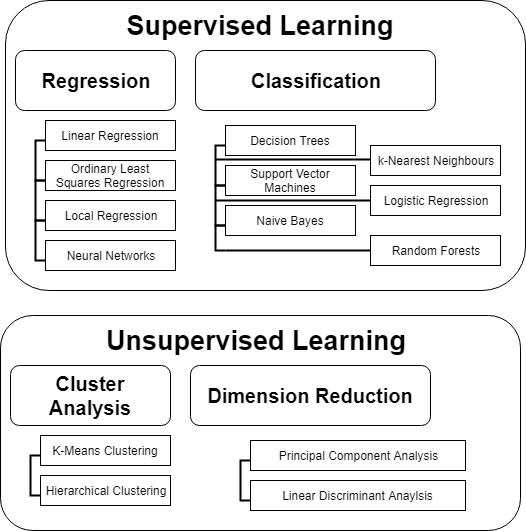
\includegraphics[width=1\linewidth]{./figures/ML_Types.png}
    \caption{Types of Machine Learning}
    \label{fig:Machine Learning Types}
\end{figure}
\end{verbatim}

    \subsection{Choosing A Machine Learning
Algorithm}\label{choosing-a-machine-learning-algorithm}

    Now that we have a general idea of what machine learning is the next
step is to choose a machine learning algorithm. To help chose the
algorithm the figure below will be utilize.

\begin{verbatim}
\begin{figure}[htbp!]
    \centering
    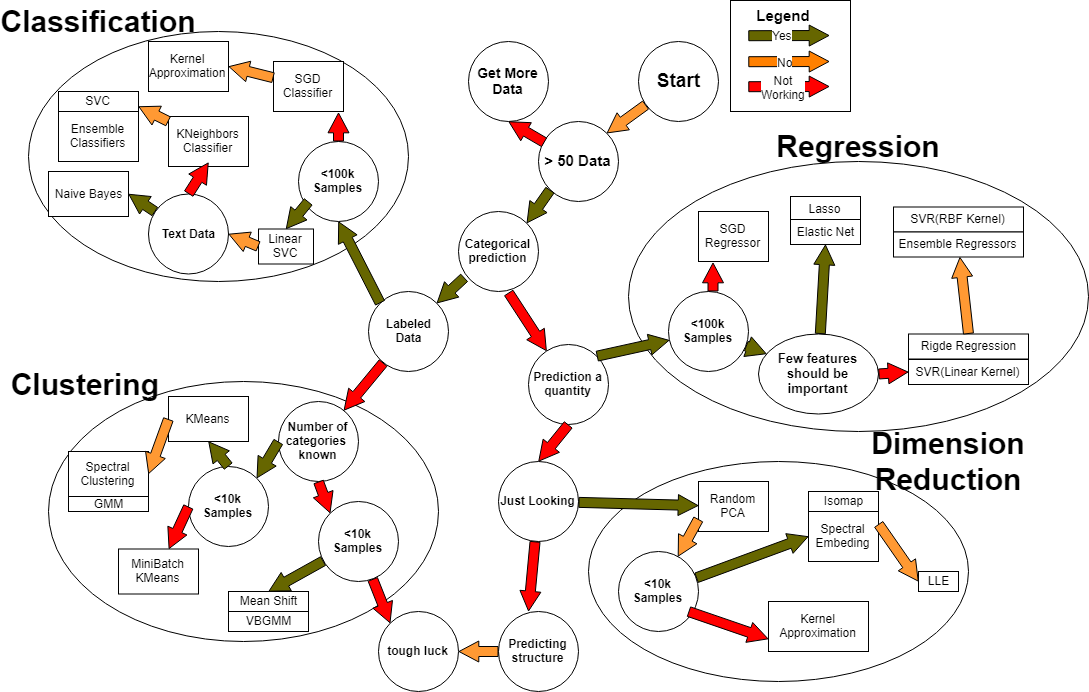
\includegraphics[width=1\linewidth]{./figures/Cheat-Sheet.png}
    \caption{Scikit Learn Algorthm Cheat-sheet}
    \label{fig:Scikit Learn Algorthm Cheat-sheet}
\end{figure}
\end{verbatim}

    \begin{enumerate}
    \item Do we have more then 50 Data - Yes
    \item Are we making a categorical prediction - At this time no, but it is possible
    \item Are we predicting a quantity - Yes, So from here we know we are looking to make a regression algorithm of some sort
    \item Do we have less the 100k sample, More then likely yes
    \item Few features should be import, all features we are looking to take advantage are important (X,Y,Z and values at known locations )
    \item Now we have an option between ridge regression and support vector regression with a linear kernel - both these methods did not work, so me move on to RBF kernels and ensemble regression
\end{enumerate}

    \subsection{Radial Basis Networks}\label{radial-basis-networks}

    In this section, the Elliptical Radial Basis Function Neural Network
(ERBFN) will be explored. This is the proposed machine learning method
to use when making a geostatistical estimation. The ERBFN is a modified
version of a Radial Basis Function Neural Network (RBFN) using
Mahalanobis distance instead of Euclidean distance. ERBFN has been used
in text-independent speak verification for example in M. W. Mak and C.
K. Li
"\textit{Elliptical Basis Function Networks and Radial Basis Function Networks for Speaker Verification: Comparative Study}."
To demonstrate why using Mahalanobis distance is preferable than using
Euclidean distance, the RBFN will first be explored, and then the ERBFN
will be explored.

Radial Basis Function Network was used by Cristian Rusu and Virginia
Rusu in
"\textit{Radial Basis Functions Versus Geostatistics in Spatial Interpolations}"
to predict the 2004 Spatial Interpolation Comparison dataset. They found
that using an RBFN generates similar results to kriging and was the best
of option for geostatistical prediction with machine learning. Due to
the similarity and ease of using an RBFN to make a prediction, they
recommended using an RBFN over kriging for spatial interpolation.

Looking at the Gaussian activation function Equation below discussed in
the previous chapter there are three things that must be decided: the
number of Gaussian kernels to be used, the radius \(r\) of each kernel,
and the location of each kernel center \(cc\). To determine the kernel
centers of each RBF k-means is first used to get an initial location of
the centers, the centers' locations are then optimized through training
the neural network. Each kernel is initialized with a width of one;
however, the radius is then optimized throughout training the neural
network by reducing the MSE of the algorithm. Finally, the number of
kernels must be selected. This is probably the most ambiguous portion of
the ML algorithm; if the number of kernels is too small the estimation
will be smooth and not be able to fit the data adequately, if the number
of kernels is too large then data will overfit and artifacts will be
introduced into the estimate. In the two Figures below a visual
representation of how the RBFN makes a prediction is illustrated in 2D
and 3D. Essentially the RBFN is the sum of multiple kernels multiplied
by a weight at the prediction location to generate an estimate.

\begin{figure}[H]
\centering
    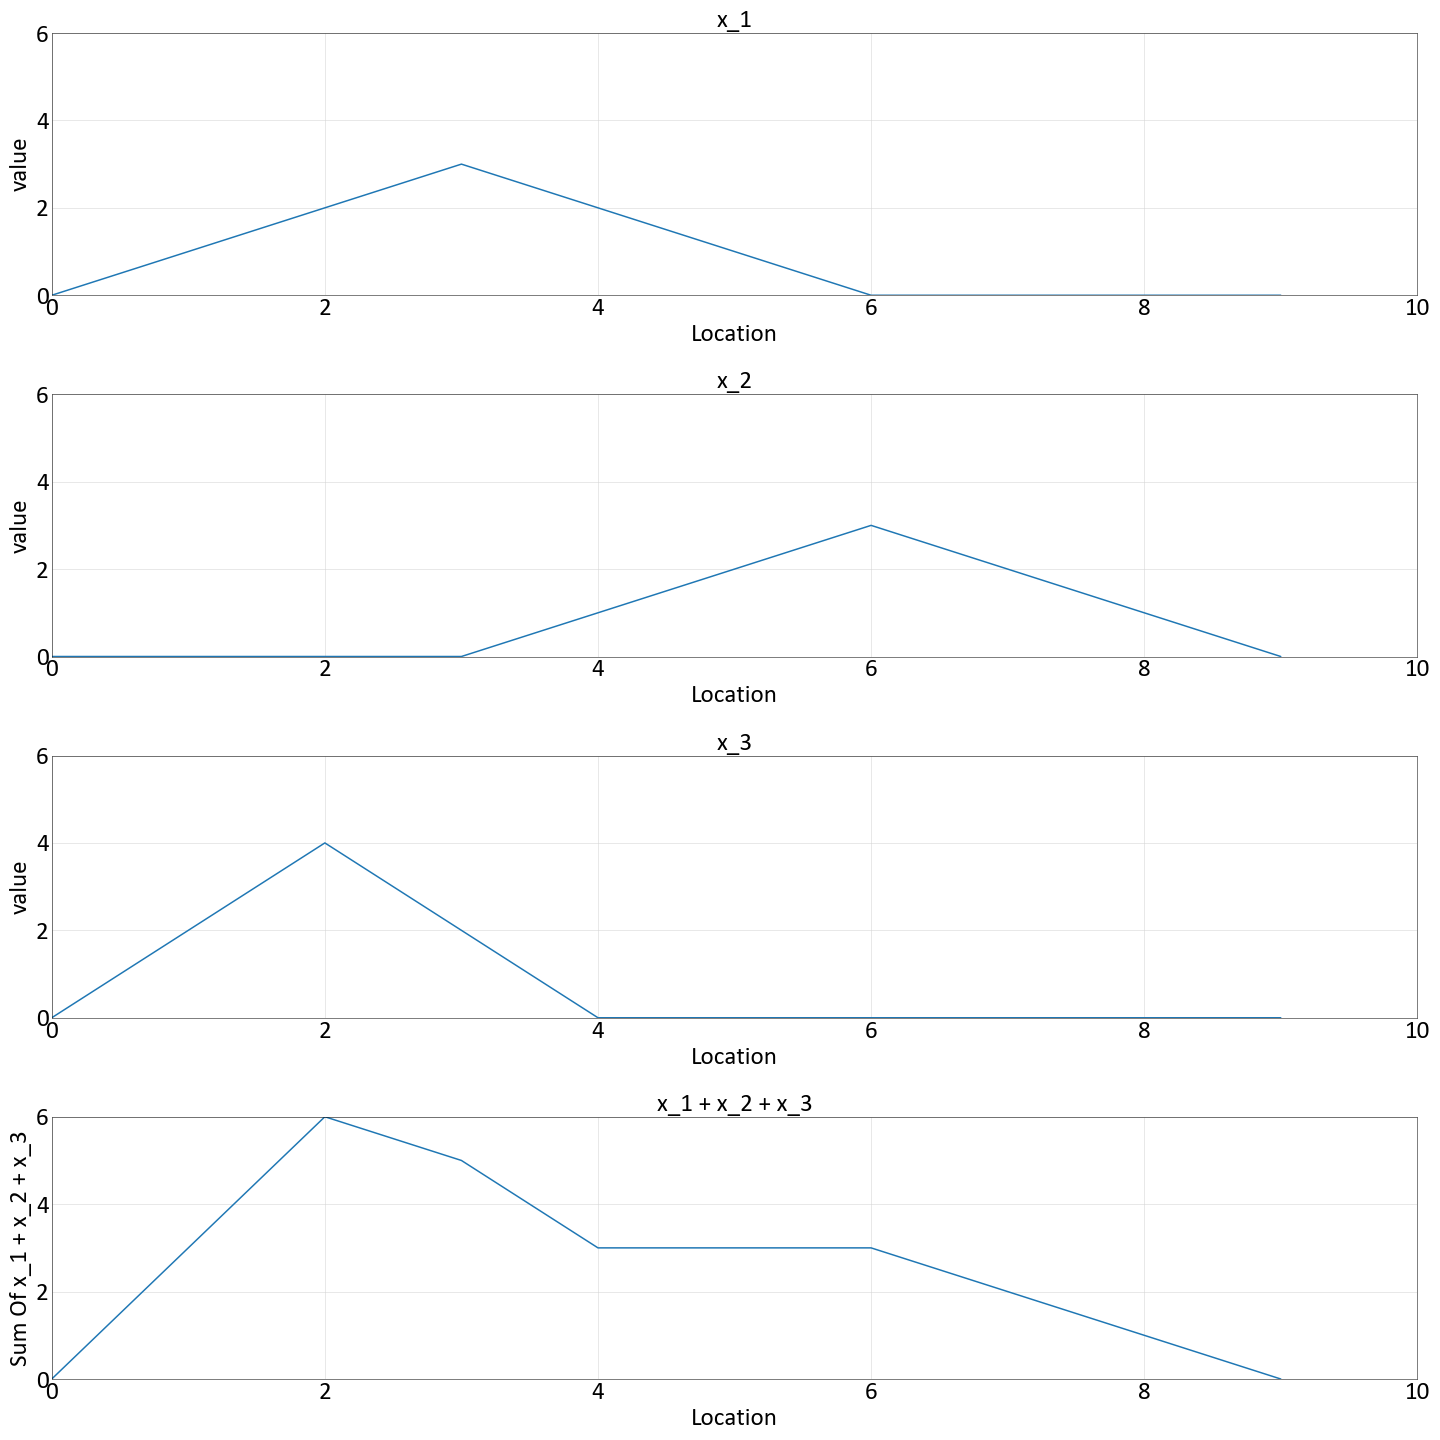
\includegraphics[width=1\linewidth]{./figures/2D_RBF.png}
  \caption{Simple RBF Example}
  \label{fig:2D RBF Example}
\end{figure}\begin{figure}[H]
\centering
    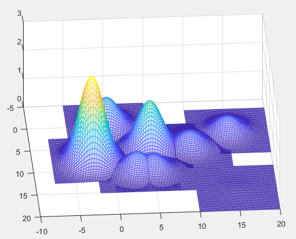
\includegraphics[width=0.75\linewidth]{./figures/3D_RBF.png}
  \caption{3D RBF Example}
  \label{fig:3D RBF Example}
\end{figure}

The matrix form of the equation also helps demonstrate this and can be
seen below in Equation \ref{eq:RBFN Matrix For Equation}.

\begin{equation}
\begin{bmatrix}
e^{-(r\left \| cc_1 - x_{1} \right \|)^2} & ... & e^{-(r\left \| cc_1 - x_{i} \right \|)^2}\\ 
\vdots  & \ddots  &\vdots \\ 
e^{-(r\left \| cc_n - x_{i} \right \|)^2} & ... & e^{-(r\left \| cc_n - x_{i} \right \|)^2}
\end{bmatrix}
\begin{bmatrix}
w_1\\ 
\vdots\\ 
w_n
\end{bmatrix}
=
\begin{bmatrix}
y_1\\ 
\vdots\\ 
y_n
\end{bmatrix}
\label{eq:RBFN Matrix For Equation}
\end{equation}

Where \(\left \| cc_n - x_{i} \right \|\) is the euclidean distance
between the cluster center and the estimation locations. An example of
how the RBFN graph looks can be seen in the figure below.

\begin{figure}[H]
\centering
    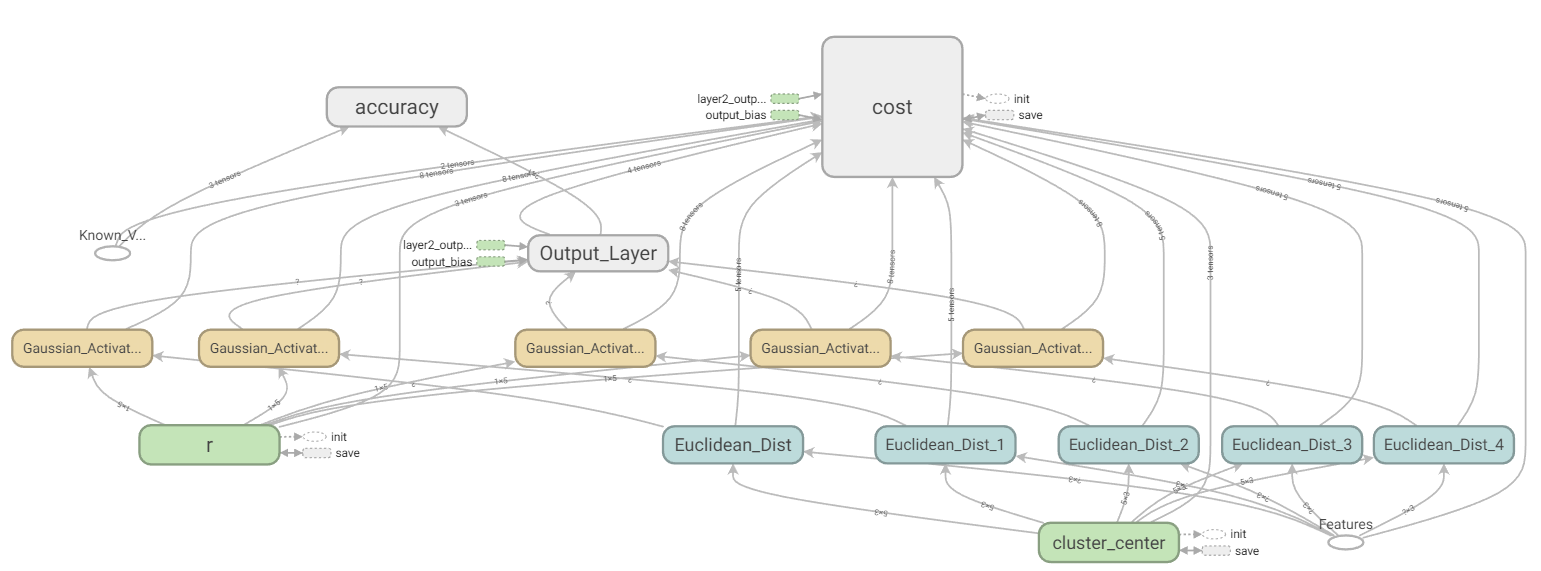
\includegraphics[width=1\linewidth]{./figures/RBFN_TensorBoard.PNG}
  \caption{Radial Basis Function Network In Tensorboard (Note each Gaussian Kernel has its own radius value $r$ ) \citep{tensorboard}}
  \label{fig:Radial Basis Function Network In Tensorboard}
\end{figure}

Now that it has been shown that ERBFN can outperform RBFN in the
non-geological example let's use the test case we started above

    \subsection{RBFN to ERBFN}\label{rbfn-to-erbfn}

    Now that the RBFN has been explored and compared to kriging the next
step is to improve upon the RBFN by converting it to an ERBFN. The
purpose of converting the RBFN to an ERBFN is to include anisotropy into
the estimation by introducing a covariance term into the estimation
using Mahalanobis distance. The ERBFN has the same structure as the RBFN
Figure above; however, the covariance is now considered. The new network
and network equation can be seen below.

\begin{figure}[H]
\centering
    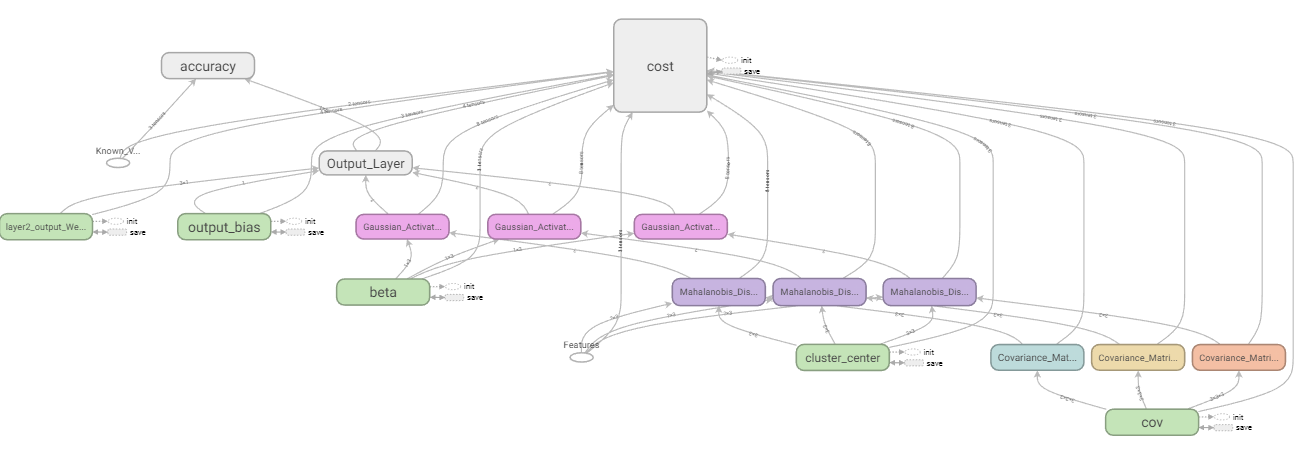
\includegraphics[width=1\linewidth]{./figures/EBFN.PNG}
  \caption{Radial Basis Function Network In Tensorboard}
  \label{fig:Radial Basis Function Network In Tensorboard}
\end{figure}

\begin{equation}
\begin{bmatrix}
e^{-(r\sqrt{d_1^T S_1^{-1} d_1})} & ... & e^{-(r\sqrt{d_1^T S_n^{-1} d_1})}\\ 
\vdots  & \ddots  &\vdots \\ 
e^{-(r\sqrt{d_i^T S_1^{-1} d_i})} & ... & e^{-(r\sqrt{d_i^T S_n^{-1} d}_i)}
\end{bmatrix}
\begin{bmatrix}
w_1\\ 
\vdots\\ 
w_n
\end{bmatrix}
=
\begin{bmatrix}
y_1\\ 
\vdots\\ 
y_n
\end{bmatrix}
\label{eq:ERBFN Matrix For Equation}
\end{equation}

Looking at the ERBFN \(S_n^{-1}\) or the covariance/shape of each kernel
is a new parameter that must be optimized by the neural network. The
covariance term is different for each kernel allowing for multiple
directions of anisotropy in a single estimation, a long with shapes that
are not spherical. Below a simple data set was simulated in 3D with
10000 data points and then sampled for 20\(\%\) of data set (2000 data
point), the sampled data was then passed through a RBFN and a ERBFN with
one node. Below it can be seen that the ERBFN better reproduces the
simulated data, RMSE equal to 0.089, as it is able to develop the
correct distribution shape due to the Mahalanobis distance; whereas, the
RBFN, RMSE 0.179, is limited to a traditional Gaussian structure using
euclidean distance.

\begin{figure}[H]
\centering
    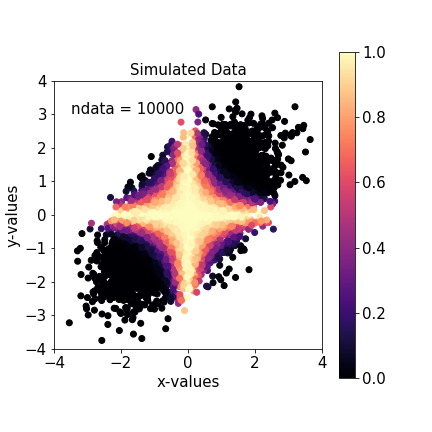
\includegraphics[width=0.5\linewidth]{./figures/SimData.png}
  \caption{Simple Simulated and Sampled Data Example for RBFN to ERBFN}
  \label{fig:Simple Simulated and Sampled Data Example for RBFN to ERBFN}
\end{figure}

\begin{figure}[H]
\centering
 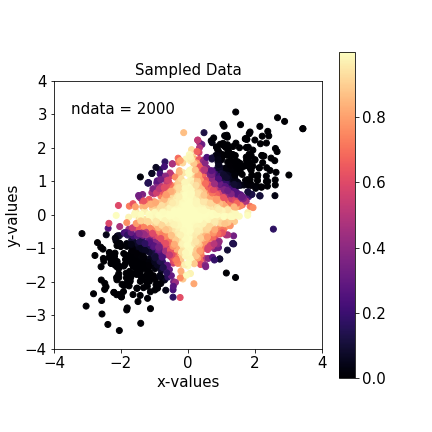
\includegraphics[width=0.5\linewidth]{./figures/SampleData.png}
  \caption{Simple Simulated and Sampled Data Example for RBFN to ERBFN}
  \label{fig:Simple Simulated and Sampled Data Example for RBFN to ERBFN}
\end{figure}

\begin{figure}[H]
\centering
    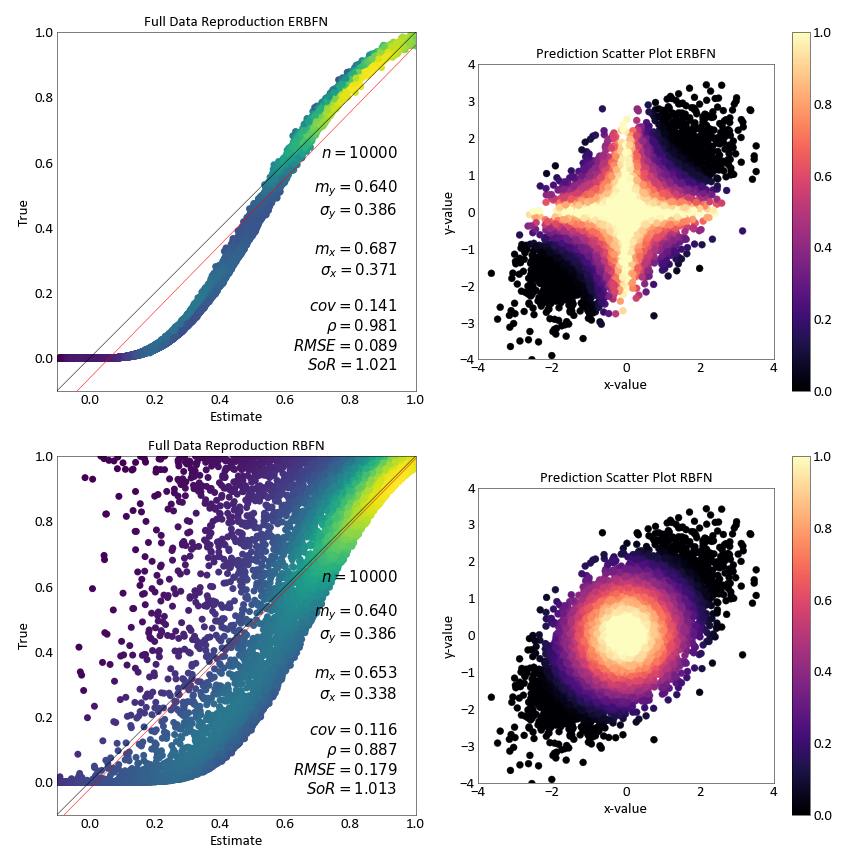
\includegraphics[width=1\linewidth]{./figures/RBFN_EBFN.png}
  \caption{Resilts From Simple Simulated and Sampled Data Example for RBFN to ERBFN}
  \label{fig:Results From Simple Simulated and Sampled Data Example for RBFN to ERBFN}
\end{figure}

Now that it has been shown that ERBFN can outperform RBFN in the
non-geological example let's use the test case from above

    \subsection{Training a machine learning
algorithm}\label{training-a-machine-learning-algorithm}

    \subsection{Machine Learning Code}\label{machine-learning-code}

    close and current tensorflow sessions that are open

    \begin{Verbatim}[commandchars=\\\{\}]
{\color{incolor}In [{\color{incolor}17}]:} \PY{k}{if} \PY{l+s+s1}{\PYZsq{}}\PY{l+s+s1}{session}\PY{l+s+s1}{\PYZsq{}} \PY{o+ow}{in} \PY{n+nb}{locals}\PY{p}{(}\PY{p}{)} \PY{o+ow}{and} \PY{n}{session} \PY{o+ow}{is} \PY{o+ow}{not} \PY{k+kc}{None}\PY{p}{:}
             \PY{n+nb}{print}\PY{p}{(}\PY{l+s+s1}{\PYZsq{}}\PY{l+s+s1}{Close interactive session}\PY{l+s+s1}{\PYZsq{}}\PY{p}{)}
             \PY{n}{session}\PY{o}{.}\PY{n}{close}\PY{p}{(}\PY{p}{)}
             \PY{n}{tf}\PY{o}{.}\PY{n}{InteractiveSession}\PY{o}{.}\PY{n}{close}\PY{p}{(}\PY{n}{sess}\PY{p}{)}
             \PY{n}{sess}\PY{o}{.}\PY{n}{close}\PY{p}{(}\PY{p}{)}
\end{Verbatim}


    setup plot settings

    \begin{Verbatim}[commandchars=\\\{\}]
{\color{incolor}In [{\color{incolor}18}]:} \PY{n}{SMALL\PYZus{}SIZE} \PY{o}{=} \PY{l+m+mi}{15}
         \PY{n}{plt}\PY{o}{.}\PY{n}{rc}\PY{p}{(}\PY{l+s+s1}{\PYZsq{}}\PY{l+s+s1}{font}\PY{l+s+s1}{\PYZsq{}}\PY{p}{,} \PY{n}{size}\PY{o}{=}\PY{n}{SMALL\PYZus{}SIZE}\PY{p}{)}
         \PY{n}{plt}\PY{o}{.}\PY{n}{rc}\PY{p}{(}\PY{l+s+s1}{\PYZsq{}}\PY{l+s+s1}{axes}\PY{l+s+s1}{\PYZsq{}}\PY{p}{,} \PY{n}{titlesize}\PY{o}{=}\PY{n}{SMALL\PYZus{}SIZE}\PY{p}{)}
\end{Verbatim}


    \subsubsection{K-Fold Validation}\label{k-fold-validation}

    After an estimation is made, the modeler must validate the estimations.
To validate the estimation, k-fold validation will be used, and then all
relevant statistics will be calculated based on each fold. In k-fold
validation, the data set will be broken into to \(k\) sets each set will
have \(\dfrac{100}{k} \%\) of the data. The estimation will then be run
\(k\) times withholding one fold of the data for testing and using the
rest of the folds for training. After all, folds have been run all
relevant statistics will be calculated based on the training and test
fold. An example of how the data would be split up can be seen below

\begin{figure}[htbp!]
        \centering
        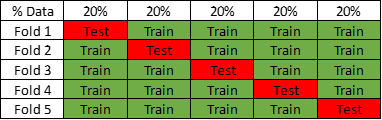
\includegraphics[width=80mm]{./figures/k_fold_ex.PNG}
        \caption[K-Fold Data Setup Example]{K-Fold Data Setup Example}
        \label{fig:K-Fold Data Setup Example}
     \end{figure}

    \begin{Verbatim}[commandchars=\\\{\}]
{\color{incolor}In [{\color{incolor}19}]:} \PY{k+kn}{from} \PY{n+nn}{sklearn}\PY{n+nn}{.}\PY{n+nn}{model\PYZus{}selection} \PY{k}{import} \PY{n}{KFold} \PY{c+c1}{\PYZsh{} import Sklearn kfold package}
         \PY{n}{kf} \PY{o}{=} \PY{n}{KFold}\PY{p}{(}\PY{n}{n\PYZus{}splits} \PY{o}{=} \PY{l+m+mi}{5}\PY{p}{,} \PY{n}{shuffle}\PY{o}{=}\PY{k+kc}{True}\PY{p}{)} \PY{c+c1}{\PYZsh{}  Specify the number of fuld and generally speaking we always want to shuffle the data}
\end{Verbatim}


    \subsubsection{Data Set up}\label{data-set-up}

    \begin{Verbatim}[commandchars=\\\{\}]
{\color{incolor}In [{\color{incolor}20}]:} \PY{c+c1}{\PYZsh{}DH Sample Data}
         \PY{n+nb}{print}\PY{p}{(}\PY{l+s+s1}{\PYZsq{}}\PY{l+s+s1}{Here we will specify the data we wish to pass to the machine algorithm and extract the min and max values from the known data   in order to scale our the values we wish to predict to be between 0 and 1}\PY{l+s+s1}{\PYZsq{}}\PY{p}{)}
         \PY{n}{datatest} \PY{o}{=} \PY{n}{np}\PY{o}{.}\PY{n}{asarray}\PY{p}{(}\PY{n}{datasamplefl}\PY{p}{)}
         \PY{n}{min\PYZus{}val} \PY{o}{=} \PY{n}{np}\PY{o}{.}\PY{n}{min}\PY{p}{(}\PY{n}{datatest}\PY{p}{[}\PY{p}{:}\PY{p}{,}\PY{l+m+mi}{3}\PY{p}{]}\PY{p}{)}
         \PY{n}{max\PYZus{}val} \PY{o}{=} \PY{n}{np}\PY{o}{.}\PY{n}{max}\PY{p}{(}\PY{n}{datatest}\PY{p}{[}\PY{p}{:}\PY{p}{,}\PY{l+m+mi}{3}\PY{p}{]}\PY{p}{)}
         \PY{n+nb}{print}\PY{p}{(}\PY{n}{min\PYZus{}val}\PY{p}{)}
         \PY{n+nb}{print}\PY{p}{(}\PY{n}{max\PYZus{}val}\PY{p}{)}
         \PY{n}{datatest}\PY{p}{[}\PY{p}{:}\PY{p}{,}\PY{l+m+mi}{3}\PY{p}{]} \PY{o}{=} \PY{p}{(}\PY{n}{datatest}\PY{p}{[}\PY{p}{:}\PY{p}{,}\PY{l+m+mi}{3}\PY{p}{]}\PY{o}{\PYZhy{}}\PY{n}{min\PYZus{}val}\PY{p}{)}\PY{o}{/}\PY{p}{(}\PY{n}{max\PYZus{}val}\PY{o}{\PYZhy{}}\PY{n}{min\PYZus{}val}\PY{p}{)}
\end{Verbatim}


    \begin{Verbatim}[commandchars=\\\{\}]
Here we will specify the data we wish to pass to the machine algorithm and extract the min and max values from the known data   in order to scale our the values we wish to predict to be between 0 and 1
-1.9313
2.9118

    \end{Verbatim}

    \begin{Verbatim}[commandchars=\\\{\}]
{\color{incolor}In [{\color{incolor}21}]:} \PY{c+c1}{\PYZsh{}Prediction Grid}
         \PY{n}{x}\PY{p}{,}\PY{n}{y}\PY{p}{,}\PY{n}{z} \PY{o}{=} \PY{n}{griddef}\PY{o}{.}\PY{n}{gridcoord}\PY{p}{(}\PY{p}{)}
         \PY{n+nb}{print}\PY{p}{(}\PY{l+s+s1}{\PYZsq{}}\PY{l+s+s1}{Generating the XYZ grid we wish to make a prediction on}\PY{l+s+s1}{\PYZsq{}}\PY{p}{)}
         \PY{n+nb}{print}\PY{p}{(}\PY{n}{x}\PY{p}{,}\PY{n}{y}\PY{p}{,}\PY{n}{z}\PY{p}{)}
         \PY{n}{data\PYZus{}x} \PY{o}{=} \PY{n}{np}\PY{o}{.}\PY{n}{hstack}\PY{p}{(}\PY{p}{(}\PY{n}{x}\PY{o}{.}\PY{n}{reshape}\PY{p}{(}\PY{n+nb}{len}\PY{p}{(}\PY{n}{x}\PY{p}{)}\PY{p}{,}\PY{l+m+mi}{1}\PY{p}{)}\PY{p}{,}\PY{n}{y}\PY{o}{.}\PY{n}{reshape}\PY{p}{(}\PY{n+nb}{len}\PY{p}{(}\PY{n}{y}\PY{p}{)}\PY{p}{,}\PY{l+m+mi}{1}\PY{p}{)}\PY{p}{,}\PY{n}{z}\PY{o}{.}\PY{n}{reshape}\PY{p}{(}\PY{n+nb}{len}\PY{p}{(}\PY{n}{z}\PY{p}{)}\PY{p}{,}\PY{l+m+mi}{1}\PY{p}{)}\PY{p}{)}\PY{p}{)}\PY{o}{/}\PY{l+m+mi}{100}
         \PY{n+nb}{print}\PY{p}{(}\PY{l+s+s1}{\PYZsq{}}\PY{l+s+s1}{the xyz values are then divide by 100 to help scale the data closer to the drill hole data values}\PY{l+s+s1}{\PYZsq{}}\PY{p}{)}
         \PY{n+nb}{print}\PY{p}{(}\PY{n}{data\PYZus{}x}\PY{p}{)}
\end{Verbatim}


    \begin{Verbatim}[commandchars=\\\{\}]
Generating the XYZ grid we wish to make a prediction on
[  5.  15.  25. {\ldots} 475. 485. 495.] [  5.   5.   5. {\ldots} 495. 495. 495.] [0.5 0.5 0.5 {\ldots} 0.5 0.5 0.5]
the xyz values are then divide by 100 to help scale the data closer to the drill hole data values
[[0.05  0.05  0.005]
 [0.15  0.05  0.005]
 [0.25  0.05  0.005]
 {\ldots}
 [4.75  4.95  0.005]
 [4.85  4.95  0.005]
 [4.95  4.95  0.005]]

    \end{Verbatim}

    \begin{Verbatim}[commandchars=\\\{\}]
{\color{incolor}In [{\color{incolor}22}]:} \PY{n}{n\PYZus{}batch} \PY{o}{=} \PY{l+m+mi}{1} 
         \PY{n+nb}{print}\PY{p}{(}\PY{l+s+s1}{\PYZsq{}}\PY{l+s+s1}{specify the number of sets to break the training data into}\PY{l+s+s1}{\PYZsq{}}\PY{p}{)}
         \PY{n+nb}{print}\PY{p}{(}\PY{l+s+s1}{\PYZsq{}}\PY{l+s+s1}{Batch Training can help reduce overfitting by cycling through different groups of the training data for each trainin epoch}\PY{l+s+s1}{\PYZsq{}}\PY{p}{)}
\end{Verbatim}


    \begin{Verbatim}[commandchars=\\\{\}]
specify the number of sets to break the training data into
Batch Training can help reduce overfitting by cycling through different groups of the training data for each trainin epoch

    \end{Verbatim}

    \begin{Verbatim}[commandchars=\\\{\}]
{\color{incolor}In [{\color{incolor}23}]:} \PY{n}{RFB\PYZus{}type} \PY{o}{=} \PY{l+s+s1}{\PYZsq{}}\PY{l+s+s1}{Gaussian}\PY{l+s+s1}{\PYZsq{}}
         \PY{n+nb}{print}\PY{p}{(}\PY{l+s+s1}{\PYZsq{}}\PY{l+s+s1}{Gaussian Kernels are currenlty the only kernel implmented}\PY{l+s+s1}{\PYZsq{}}\PY{p}{)}
\end{Verbatim}


    \begin{Verbatim}[commandchars=\\\{\}]
Gaussian Kernels are currenlty the only kernel implmented

    \end{Verbatim}

    \begin{Verbatim}[commandchars=\\\{\}]
{\color{incolor}In [{\color{incolor}24}]:} \PY{n}{display\PYZus{}step} \PY{o}{=} \PY{l+m+mi}{50}
         \PY{n+nb}{print}\PY{p}{(}\PY{l+s+s1}{\PYZsq{}}\PY{l+s+s1}{The training and testint error will be calcualted ever }\PY{l+s+si}{\PYZob{}\PYZcb{}}\PY{l+s+s1}{ training epochs along with a graph to track the progress}\PY{l+s+s1}{\PYZsq{}}\PY{o}{.}\PY{n}{format}\PY{p}{(}\PY{n}{display\PYZus{}step}\PY{p}{)}\PY{p}{)}
\end{Verbatim}


    \begin{Verbatim}[commandchars=\\\{\}]
The training and testint error will be calcualted ever 50 training epochs along with a graph to track the progress

    \end{Verbatim}

    \begin{Verbatim}[commandchars=\\\{\}]
{\color{incolor}In [{\color{incolor}25}]:} \PY{n}{test\PYZus{}nodes} \PY{o}{=} \PY{p}{[}\PY{l+m+mi}{20}\PY{p}{]}
         \PY{n+nb}{print}\PY{p}{(}\PY{l+s+s1}{\PYZsq{}}\PY{l+s+s1}{test\PYZus{}nodes can be set to a range of RBF nodes (eg.[10,20,30]) and the solution provided will be an esemble}\PY{l+s+s1}{\PYZsq{}}\PY{p}{)}
         \PY{n+nb}{print}\PY{p}{(}\PY{l+s+s1}{\PYZsq{}}\PY{l+s+s1}{typically ensemble solutions are better then a single node solution}\PY{l+s+s1}{\PYZsq{}}\PY{p}{)}
\end{Verbatim}


    \begin{Verbatim}[commandchars=\\\{\}]
test\_nodes can be set to a range of RBF nodes (eg.[10,20,30]) and the solution provided will be an esemble
typically ensemble solutions are better then a single node solution

    \end{Verbatim}

    \begin{Verbatim}[commandchars=\\\{\}]
{\color{incolor}In [{\color{incolor}26}]:} \PY{n}{learning\PYZus{}rate} \PY{o}{=} \PY{l+m+mf}{0.01}
         \PY{n}{training\PYZus{}epochs} \PY{o}{=} \PY{l+m+mi}{4000}
         
         \PY{n+nb}{print}\PY{p}{(}\PY{l+s+s1}{\PYZsq{}}\PY{l+s+s1}{typically a learning rate of 0.01 is reasonable; however, this is subject to change based on the problem}\PY{l+s+s1}{\PYZsq{}}\PY{p}{)}
         \PY{n+nb}{print}\PY{p}{(}\PY{l+s+s1}{\PYZsq{}}\PY{l+s+s1}{trainig\PYZus{}epochs is proportional to the learning rate, the higher the learning reate the lower the number of epochs required; again the number of learning epochs can change based on the problem}\PY{l+s+s1}{\PYZsq{}}\PY{p}{)}
\end{Verbatim}


    \begin{Verbatim}[commandchars=\\\{\}]
typically a learning rate of 0.01 is reasonable; however, this is subject to change based on the problem
trainig\_epochs is proportional to the learning rate, the higher the learning reate the lower the number of epochs required; again the number of learning epochs can change based on the problem

    \end{Verbatim}

    \subsubsection{What to Look For While
Training}\label{what-to-look-for-while-training}

    While an estimation is training ideally the test and training set
exhibit similar error, if the train and testing error is significantly
different this would suggest the algorithm has over fit the data. While
training if we see the training and testing data set have similar error
and the start to diverge this would indicate an early stop. In general
we want to see both the training and testing set decreasing in error
together.

\begin{verbatim}
\begin{figure}[htbp!]
    \centering
    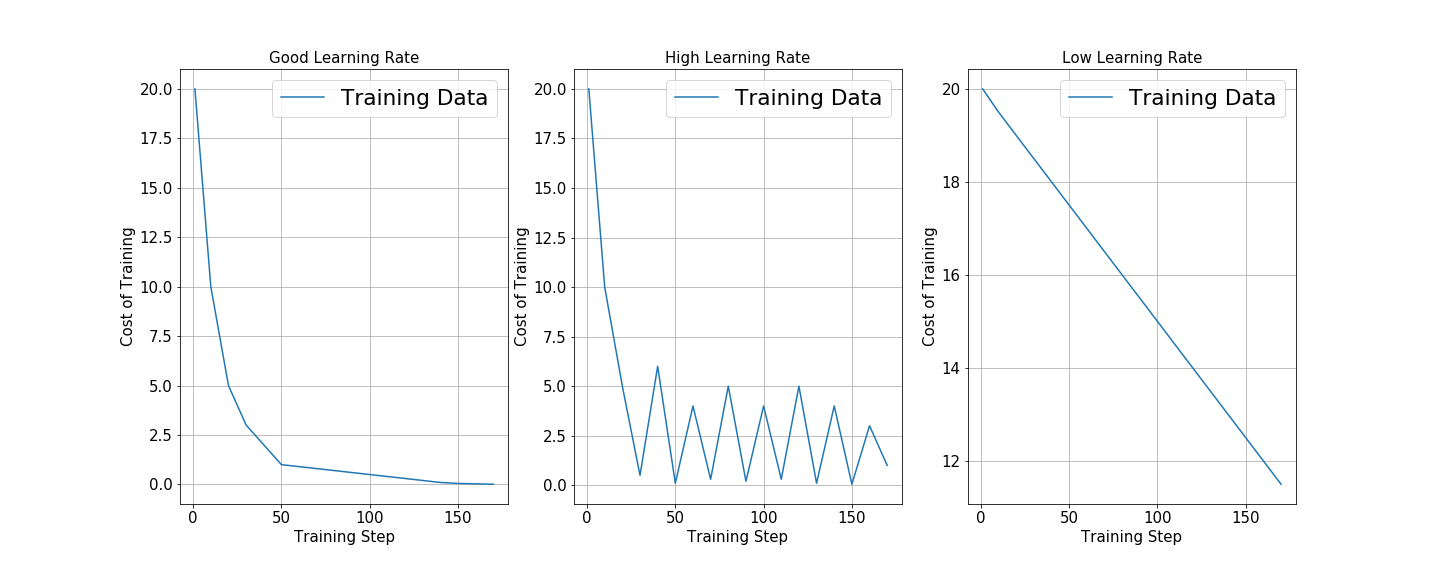
\includegraphics[width=80mm]{./figures/Training_cost_training_error.png}
 \end{figure}
 
\begin{figure}[htbp!]
    \centering
    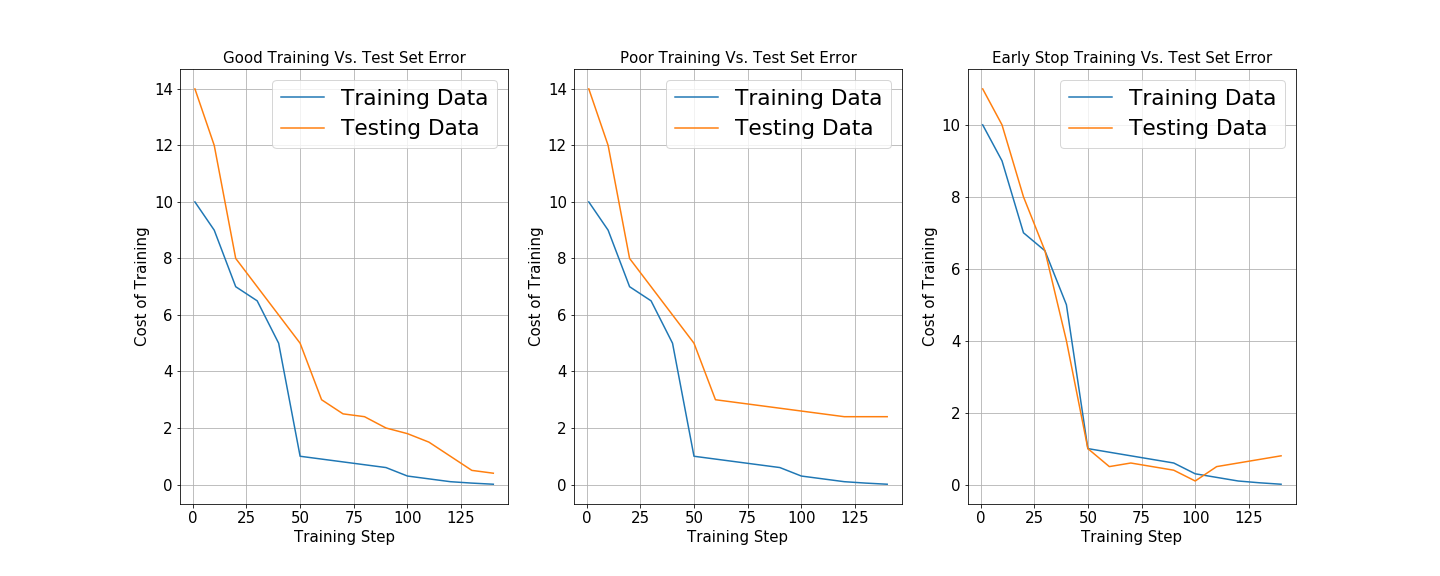
\includegraphics[width=80mm]{./figures/Training_vs_test_cost.png}
 \end{figure}
 
\begin{figure}[htbp!]
    \centering
    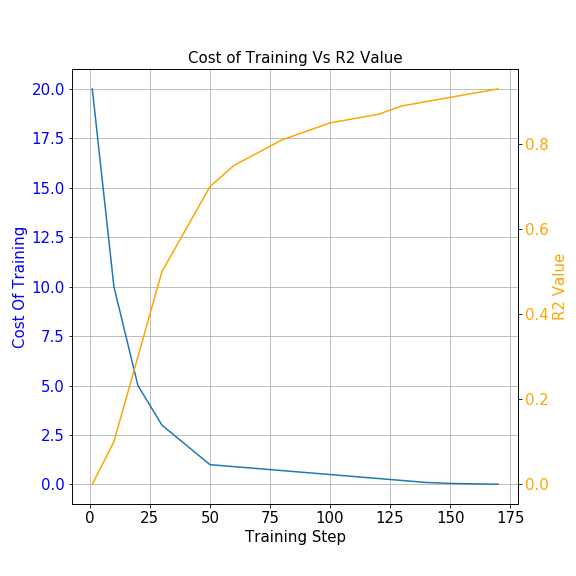
\includegraphics[width=30mm]{./figures/Training_R2.png}
 \end{figure}
\end{verbatim}

    \subsubsection{ERBFN}\label{erbfn}

    \begin{Verbatim}[commandchars=\\\{\}]
{\color{incolor}In [{\color{incolor}27}]:} \PY{n}{columns} \PY{o}{=} \PY{p}{[}\PY{l+s+s1}{\PYZsq{}}\PY{l+s+s1}{X}\PY{l+s+s1}{\PYZsq{}}\PY{p}{,}\PY{l+s+s1}{\PYZsq{}}\PY{l+s+s1}{Y}\PY{l+s+s1}{\PYZsq{}}\PY{p}{,}\PY{l+s+s1}{\PYZsq{}}\PY{l+s+s1}{Z}\PY{l+s+s1}{\PYZsq{}}\PY{p}{,}\PY{l+s+s1}{\PYZsq{}}\PY{l+s+s1}{value}\PY{l+s+s1}{\PYZsq{}}\PY{p}{]}
         \PY{n}{fold\PYZus{}num}\PY{o}{=} \PY{l+m+mi}{0}
         \PY{n}{kf}\PY{o}{.}\PY{n}{get\PYZus{}n\PYZus{}splits}\PY{p}{(}\PY{n}{datatest}\PY{p}{)}
         \PY{k}{for} \PY{n}{train\PYZus{}index}\PY{p}{,} \PY{n}{test\PYZus{}index} \PY{o+ow}{in} \PY{n}{kf}\PY{o}{.}\PY{n}{split}\PY{p}{(}\PY{n}{datatest}\PY{p}{)}\PY{p}{:}
             \PY{n}{fold\PYZus{}num} \PY{o}{+}\PY{o}{=} \PY{l+m+mi}{1}
             \PY{n+nb}{print}\PY{p}{(}\PY{n}{fold\PYZus{}num}\PY{p}{)}
             \PY{c+c1}{\PYZsh{}print(\PYZdq{}TRAIN:\PYZdq{}, train\PYZus{}index, \PYZdq{}TEST:\PYZdq{}, test\PYZus{}index)}
             \PY{n}{data\PYZus{}train}\PY{p}{,} \PY{n}{data\PYZus{}test} \PY{o}{=} \PY{n}{datatest}\PY{p}{[}\PY{n}{train\PYZus{}index}\PY{p}{,}\PY{l+m+mi}{0}\PY{p}{:}\PY{l+m+mi}{3}\PY{p}{]}\PY{o}{/}\PY{l+m+mi}{100}\PY{p}{,} \PY{n}{datatest}\PY{p}{[}\PY{n}{test\PYZus{}index}\PY{p}{,}\PY{l+m+mi}{0}\PY{p}{:}\PY{l+m+mi}{3}\PY{p}{]}\PY{o}{/}\PY{l+m+mi}{100}
             \PY{n}{target\PYZus{}train}\PY{p}{,} \PY{n}{target\PYZus{}test} \PY{o}{=} \PY{n}{datatest}\PY{p}{[}\PY{n}{train\PYZus{}index}\PY{p}{,}\PY{l+m+mi}{3}\PY{p}{:}\PY{l+m+mi}{4}\PY{p}{]}\PY{p}{,} \PY{n}{datatest}\PY{p}{[}\PY{n}{test\PYZus{}index}\PY{p}{,}\PY{l+m+mi}{3}\PY{p}{:}\PY{l+m+mi}{4}\PY{p}{]}
             \PY{n}{gs}\PY{o}{.}\PY{n}{write\PYZus{}gslib}\PY{p}{(}\PY{n}{pd}\PY{o}{.}\PY{n}{DataFrame}\PY{p}{(}\PY{n}{np}\PY{o}{.}\PY{n}{hstack}\PY{p}{(}\PY{p}{(}\PY{n}{data\PYZus{}train}\PY{o}{*}\PY{l+m+mi}{100}\PY{p}{,}\PY{n}{target\PYZus{}train}\PY{o}{*}\PY{p}{(}\PY{n}{max\PYZus{}val}\PY{o}{\PYZhy{}}\PY{n}{min\PYZus{}val}\PY{p}{)}\PY{o}{+}\PY{n}{min\PYZus{}val}\PY{p}{)}\PY{p}{)}\PY{p}{,}\PY{n}{columns}\PY{o}{=}\PY{n}{columns}\PY{p}{)}\PY{p}{,} \PY{l+s+s1}{\PYZsq{}}\PY{l+s+s1}{./data/data\PYZus{}train\PYZus{}}\PY{l+s+si}{\PYZob{}\PYZcb{}}\PY{l+s+s1}{.dat}\PY{l+s+s1}{\PYZsq{}}\PY{o}{.}\PY{n}{format}\PY{p}{(}\PY{n}{fold\PYZus{}num}\PY{p}{)}\PY{p}{)}
             \PY{n}{gs}\PY{o}{.}\PY{n}{write\PYZus{}gslib}\PY{p}{(}\PY{n}{pd}\PY{o}{.}\PY{n}{DataFrame}\PY{p}{(}\PY{n}{np}\PY{o}{.}\PY{n}{hstack}\PY{p}{(}\PY{p}{(}\PY{n}{data\PYZus{}test}\PY{o}{*}\PY{l+m+mi}{100}\PY{p}{,}\PY{n}{target\PYZus{}test}\PY{o}{*}\PY{p}{(}\PY{n}{max\PYZus{}val}\PY{o}{\PYZhy{}}\PY{n}{min\PYZus{}val}\PY{p}{)}\PY{o}{+}\PY{n}{min\PYZus{}val}\PY{p}{)}\PY{p}{)}\PY{p}{,}\PY{n}{columns}\PY{o}{=}\PY{n}{columns}\PY{p}{)}\PY{p}{,} \PY{l+s+s1}{\PYZsq{}}\PY{l+s+s1}{./data/data\PYZus{}test\PYZus{}}\PY{l+s+si}{\PYZob{}\PYZcb{}}\PY{l+s+s1}{.dat}\PY{l+s+s1}{\PYZsq{}}\PY{o}{.}\PY{n}{format}\PY{p}{(}\PY{n}{fold\PYZus{}num}\PY{p}{)}\PY{p}{)}
             \PY{n}{row} \PY{o}{=} \PY{l+m+mi}{0}
             \PY{n}{NN} \PY{o}{=} \PY{l+s+s1}{\PYZsq{}}\PY{l+s+s1}{ERBFN}\PY{l+s+s1}{\PYZsq{}} \PY{c+c1}{\PYZsh{} RBFN or GRNN or \PYZsq{}EBFN\PYZsq{}}
             \PY{n}{data\PYZus{}type} \PY{o}{=} \PY{l+s+s1}{\PYZsq{}}\PY{l+s+s1}{Continuous}\PY{l+s+s1}{\PYZsq{}} \PY{c+c1}{\PYZsh{} Continuous or Categorical}
             \PY{n}{test\PYZus{}nodes} \PY{o}{=} \PY{n}{test\PYZus{}nodes}
             \PY{n}{pred\PYZus{}all} \PY{o}{=} \PY{n}{np}\PY{o}{.}\PY{n}{zeros}\PY{p}{(}\PY{p}{(}\PY{n+nb}{len}\PY{p}{(}\PY{n}{test\PYZus{}nodes}\PY{p}{)}\PY{o}{*}\PY{n}{data\PYZus{}x}\PY{o}{.}\PY{n}{shape}\PY{p}{[}\PY{l+m+mi}{0}\PY{p}{]}\PY{p}{,}\PY{n}{target\PYZus{}train}\PY{o}{.}\PY{n}{shape}\PY{p}{[}\PY{l+m+mi}{1}\PY{p}{]}\PY{p}{)}\PY{p}{)}
             \PY{n}{pred\PYZus{}all\PYZus{}row} \PY{o}{=} \PY{n}{np}\PY{o}{.}\PY{n}{zeros}\PY{p}{(}\PY{p}{(}\PY{n}{data\PYZus{}x}\PY{o}{.}\PY{n}{shape}\PY{p}{[}\PY{l+m+mi}{0}\PY{p}{]}\PY{p}{,}\PY{n}{target\PYZus{}train}\PY{o}{.}\PY{n}{shape}\PY{p}{[}\PY{l+m+mi}{1}\PY{p}{]}\PY{p}{,}\PY{n+nb}{len}\PY{p}{(}\PY{n}{test\PYZus{}nodes}\PY{p}{)}\PY{p}{)}\PY{p}{)}
             \PY{n}{info\PYZus{}matrix} \PY{o}{=} \PY{n}{np}\PY{o}{.}\PY{n}{zeros}\PY{p}{(}\PY{p}{(}\PY{n+nb}{len}\PY{p}{(}\PY{n}{test\PYZus{}nodes}\PY{p}{)}\PY{p}{,}\PY{l+m+mi}{8}\PY{p}{)}\PY{p}{)}
             \PY{k}{for} \PY{n}{nodes} \PY{o+ow}{in} \PY{n}{test\PYZus{}nodes}\PY{p}{:}
                 \PY{n}{c\PYZus{}t} \PY{o}{=} \PY{p}{[}\PY{p}{]}
                 \PY{n}{c\PYZus{}test} \PY{o}{=} \PY{p}{[}\PY{p}{]}
                 \PY{n}{c\PYZus{}r2} \PY{o}{=} \PY{p}{[}\PY{p}{]}
                 \PY{n}{epoch\PYZus{}plt} \PY{o}{=} \PY{p}{[}\PY{p}{]}
                 \PY{n}{start\PYZus{}time} \PY{o}{=} \PY{n}{time}\PY{o}{.}\PY{n}{time}\PY{p}{(}\PY{p}{)}
                 \PY{n+nb}{print}\PY{p}{(}\PY{l+s+s2}{\PYZdq{}}\PY{l+s+s2}{Working on Node }\PY{l+s+si}{\PYZob{}\PYZcb{}}\PY{l+s+s2}{ fold }\PY{l+s+si}{\PYZob{}\PYZcb{}}\PY{l+s+s2}{ }\PY{l+s+s2}{\PYZdq{}}\PY{o}{.}\PY{n}{format}\PY{p}{(}\PY{n}{nodes}\PY{p}{,}\PY{n}{fold\PYZus{}num}\PY{p}{)}\PY{p}{)}
                 \PY{n}{k} \PY{o}{=} \PY{n}{nodes}
                 \PY{n}{data\PYZus{}trainpd} \PY{o}{=} \PY{n}{pd}\PY{o}{.}\PY{n}{DataFrame}\PY{p}{(}\PY{n}{data\PYZus{}train}\PY{p}{)}
                 \PY{n}{data} \PY{o}{=} \PY{n}{data\PYZus{}trainpd}
         
                 \PY{k}{with} \PY{n}{tf}\PY{o}{.}\PY{n}{device}\PY{p}{(}\PY{l+s+s1}{\PYZsq{}}\PY{l+s+s1}{/device:CPU:0}\PY{l+s+s1}{\PYZsq{}}\PY{p}{)}\PY{p}{:}
                     \PY{c+c1}{\PYZsh{}clustering}
                     \PY{k}{def} \PY{n+nf}{input\PYZus{}fn}\PY{p}{(}\PY{p}{)}\PY{p}{:}
                       \PY{k}{return} \PY{n}{tf}\PY{o}{.}\PY{n}{train}\PY{o}{.}\PY{n}{limit\PYZus{}epochs}\PY{p}{(}
                           \PY{n}{tf}\PY{o}{.}\PY{n}{convert\PYZus{}to\PYZus{}tensor}\PY{p}{(}\PY{n}{data\PYZus{}train}\PY{p}{,} \PY{n}{dtype}\PY{o}{=}\PY{n}{tf}\PY{o}{.}\PY{n}{float32}\PY{p}{)}\PY{p}{,} \PY{n}{num\PYZus{}epochs}\PY{o}{=}\PY{l+m+mi}{1}\PY{p}{)}
         
                     \PY{n}{kmeans} \PY{o}{=} \PY{n}{tf}\PY{o}{.}\PY{n}{contrib}\PY{o}{.}\PY{n}{factorization}\PY{o}{.}\PY{n}{KMeansClustering}\PY{p}{(}
                         \PY{n}{num\PYZus{}clusters}\PY{o}{=}\PY{n}{nodes}\PY{p}{,} \PY{n}{use\PYZus{}mini\PYZus{}batch}\PY{o}{=}\PY{k+kc}{False}\PY{p}{)}
         
         
                     \PY{c+c1}{\PYZsh{} train}
                     \PY{n}{num\PYZus{}iterations} \PY{o}{=} \PY{l+m+mi}{10}
                     \PY{n}{previous\PYZus{}centers} \PY{o}{=} \PY{k+kc}{None}
                     \PY{k}{for} \PY{n}{\PYZus{}} \PY{o+ow}{in} \PY{n+nb}{range}\PY{p}{(}\PY{n}{num\PYZus{}iterations}\PY{p}{)}\PY{p}{:}
                       \PY{n}{kmeans}\PY{o}{.}\PY{n}{train}\PY{p}{(}\PY{n}{input\PYZus{}fn}\PY{p}{)}
                       \PY{n}{cluster\PYZus{}centers} \PY{o}{=} \PY{n}{kmeans}\PY{o}{.}\PY{n}{cluster\PYZus{}centers}\PY{p}{(}\PY{p}{)}
                       \PY{c+c1}{\PYZsh{}if previous\PYZus{}centers is not None:}
                         \PY{c+c1}{\PYZsh{}print(\PYZsq{}delta:\PYZsq{}, cluster\PYZus{}centers \PYZhy{} previous\PYZus{}centers)}
                       \PY{n}{previous\PYZus{}centers} \PY{o}{=} \PY{n}{cluster\PYZus{}centers}
                       \PY{c+c1}{\PYZsh{}print(\PYZsq{}score:\PYZsq{}, kmeans.score(input\PYZus{}fn))}
                     \PY{c+c1}{\PYZsh{}print(\PYZsq{}cluster centers:\PYZsq{}, cluster\PYZus{}centers)}
                     
                     
                 \PY{k}{with} \PY{n}{tf}\PY{o}{.}\PY{n}{device}\PY{p}{(}\PY{l+s+s1}{\PYZsq{}}\PY{l+s+s1}{/device:GPU:0}\PY{l+s+s1}{\PYZsq{}}\PY{p}{)}\PY{p}{:}
                     \PY{k+kn}{from} \PY{n+nn}{tensorflow}\PY{n+nn}{.}\PY{n+nn}{python}\PY{n+nn}{.}\PY{n+nn}{framework} \PY{k}{import} \PY{n}{ops}
                     \PY{n}{ops}\PY{o}{.}\PY{n}{reset\PYZus{}default\PYZus{}graph}\PY{p}{(}\PY{p}{)}
         
         
                     \PY{n}{RANDOM\PYZus{}SEED} \PY{o}{=} \PY{l+m+mi}{42}
                     \PY{n}{tf}\PY{o}{.}\PY{n}{set\PYZus{}random\PYZus{}seed}\PY{p}{(}\PY{n}{RANDOM\PYZus{}SEED}\PY{p}{)}
         
                     \PY{n}{N\PYZus{}INSTANCES} \PY{o}{=} \PY{n}{np}\PY{o}{.}\PY{n}{shape}\PY{p}{(}\PY{n}{data\PYZus{}train}\PY{p}{)}\PY{p}{[}\PY{l+m+mi}{0}\PY{p}{]}
                     \PY{n}{N\PYZus{}INPUT} \PY{o}{=} \PY{n}{data\PYZus{}train}\PY{o}{.}\PY{n}{shape}\PY{p}{[}\PY{l+m+mi}{0}\PY{p}{]}
                     \PY{n}{N\PYZus{}FEATURE} \PY{o}{=} \PY{n}{data\PYZus{}train}\PY{o}{.}\PY{n}{shape}\PY{p}{[}\PY{l+m+mi}{1}\PY{p}{]}
                     \PY{n}{N\PYZus{}CLASSES} \PY{o}{=} \PY{n}{target\PYZus{}train}\PY{o}{.}\PY{n}{shape}\PY{p}{[}\PY{l+m+mi}{1}\PY{p}{]}
                     \PY{n}{TRAIN\PYZus{}SIZE} \PY{o}{=} \PY{n+nb}{int}\PY{p}{(}\PY{n}{N\PYZus{}INSTANCES}\PY{p}{)}
                     \PY{n}{batch\PYZus{}size} \PY{o}{=} \PY{n+nb}{int}\PY{p}{(}\PY{n}{np}\PY{o}{.}\PY{n}{shape}\PY{p}{(}\PY{n}{data\PYZus{}train}\PY{p}{)}\PY{p}{[}\PY{l+m+mi}{0}\PY{p}{]}\PY{o}{/}\PY{n}{n\PYZus{}batch}\PY{p}{)}
                     \PY{n}{training\PYZus{}epochs} \PY{o}{=} \PY{n}{training\PYZus{}epochs}
                     \PY{k}{if} \PY{n}{nodes} \PY{o}{\PYZgt{}}\PY{o}{=} \PY{l+m+mi}{2}\PY{p}{:}
                         \PY{n}{training\PYZus{}epochs} \PY{o}{=} \PY{n}{training\PYZus{}epochs}
                     \PY{k}{if} \PY{n}{nodes} \PY{o}{\PYZgt{}}\PY{o}{=} \PY{l+m+mi}{25}\PY{p}{:}
                         \PY{n}{training\PYZus{}epochs} \PY{o}{=} \PY{n}{training\PYZus{}epochs}
                     \PY{k}{if} \PY{n}{nodes} \PY{o}{\PYZgt{}}\PY{o}{=} \PY{l+m+mi}{100}\PY{p}{:}
                         \PY{n}{training\PYZus{}epochs} \PY{o}{=} \PY{n}{training\PYZus{}epochs}
                     \PY{k}{if} \PY{n}{nodes} \PY{o}{\PYZgt{}}\PY{o}{=} \PY{l+m+mi}{1000}\PY{p}{:}
                         \PY{n}{training\PYZus{}epochs} \PY{o}{=} \PY{n}{training\PYZus{}epochs}
                     \PY{n}{learning\PYZus{}rate} \PY{o}{=} \PY{n}{learning\PYZus{}rate}
                     \PY{n}{epsilon} \PY{o}{=} \PY{l+m+mf}{0.001}
                     \PY{n}{display\PYZus{}step} \PY{o}{=} \PY{n}{display\PYZus{}step}
                     \PY{n}{hidden\PYZus{}size} \PY{o}{=} \PY{n}{nodes}
         
                     \PY{n}{target\PYZus{}} \PY{o}{=} \PY{n}{np}\PY{o}{.}\PY{n}{zeros}\PY{p}{(}\PY{p}{(}\PY{n}{N\PYZus{}INSTANCES}\PY{p}{,} \PY{n}{N\PYZus{}CLASSES}\PY{p}{)}\PY{p}{)}
                     \PY{n}{extra\PYZus{}update\PYZus{}ops} \PY{o}{=} \PY{n}{tf}\PY{o}{.}\PY{n}{get\PYZus{}collection}\PY{p}{(}\PY{n}{tf}\PY{o}{.}\PY{n}{GraphKeys}\PY{o}{.}\PY{n}{UPDATE\PYZus{}OPS}\PY{p}{)}
         
                     \PY{n}{x\PYZus{}data} \PY{o}{=} \PY{n}{tf}\PY{o}{.}\PY{n}{placeholder}\PY{p}{(}\PY{n}{shape}\PY{o}{=}\PY{p}{[}\PY{k+kc}{None}\PY{p}{,} \PY{n}{N\PYZus{}FEATURE}\PY{p}{]}\PY{p}{,} \PY{n}{dtype}\PY{o}{=}\PY{n}{tf}\PY{o}{.}\PY{n}{float32}\PY{p}{,} \PY{n}{name} \PY{o}{=} \PY{l+s+s1}{\PYZsq{}}\PY{l+s+s1}{Features}\PY{l+s+s1}{\PYZsq{}}\PY{p}{)}
                     \PY{n}{y\PYZus{}target} \PY{o}{=} \PY{n}{tf}\PY{o}{.}\PY{n}{placeholder}\PY{p}{(}\PY{n}{shape}\PY{o}{=}\PY{p}{[}\PY{k+kc}{None}\PY{p}{,} \PY{n}{N\PYZus{}CLASSES}\PY{p}{]}\PY{p}{,} \PY{n}{dtype}\PY{o}{=}\PY{n}{tf}\PY{o}{.}\PY{n}{float32}\PY{p}{,} \PY{n}{name} \PY{o}{=} \PY{l+s+s1}{\PYZsq{}}\PY{l+s+s1}{Known\PYZus{}Values}\PY{l+s+s1}{\PYZsq{}}\PY{p}{)}
         
         
                     \PY{n}{dist} \PY{o}{=} \PY{n}{np}\PY{o}{.}\PY{n}{zeros}\PY{p}{(}\PY{p}{(}\PY{n}{k}\PY{p}{,}\PY{n}{k}\PY{p}{)}\PY{p}{)}
                     \PY{k}{for} \PY{n}{i} \PY{o+ow}{in} \PY{n+nb}{range} \PY{p}{(}\PY{l+m+mi}{0}\PY{p}{,}\PY{n}{k}\PY{p}{)}\PY{p}{:}
                         \PY{k}{for} \PY{n}{j} \PY{o+ow}{in} \PY{n+nb}{range} \PY{p}{(}\PY{l+m+mi}{0}\PY{p}{,}\PY{n}{k}\PY{p}{)}\PY{p}{:}
                             \PY{n}{dist}\PY{p}{[}\PY{n}{i}\PY{p}{:}\PY{n}{j}\PY{p}{]} \PY{o}{=} \PY{n}{distance}\PY{o}{.}\PY{n}{euclidean}\PY{p}{(}\PY{n}{cluster\PYZus{}centers}\PY{p}{[}\PY{n}{i}\PY{p}{]}\PY{p}{,} \PY{n}{cluster\PYZus{}centers}\PY{p}{[}\PY{n}{j}\PY{p}{]}\PY{p}{)}
                             \PY{n}{maxdist} \PY{o}{=} \PY{n}{dist}\PY{o}{.}\PY{n}{max}\PY{p}{(}\PY{p}{)}
                     \PY{n}{sigma} \PY{o}{=} \PY{n}{maxdist}\PY{o}{/}\PY{n}{np}\PY{o}{.}\PY{n}{sqrt}\PY{p}{(}\PY{l+m+mi}{2}\PY{o}{*}\PY{n}{k}\PY{p}{)}
                     \PY{k}{if} \PY{n}{nodes} \PY{o}{==} \PY{l+m+mi}{1} \PY{p}{:}
                         \PY{n}{beta} \PY{o}{=} \PY{l+m+mf}{0.2}
                     \PY{k}{else}\PY{p}{:}        
                         \PY{n}{beta} \PY{o}{=} \PY{l+m+mi}{1}\PY{o}{/}\PY{n}{math}\PY{o}{.}\PY{n}{pow}\PY{p}{(}\PY{l+m+mi}{2}\PY{o}{*}\PY{n}{sigma}\PY{p}{,}\PY{l+m+mi}{2}\PY{p}{)}
         
                     \PY{c+c1}{\PYZsh{}EBFN}
                     \PY{k}{if} \PY{n}{NN} \PY{o}{==} \PY{l+s+s1}{\PYZsq{}}\PY{l+s+s1}{ERBFN}\PY{l+s+s1}{\PYZsq{}}\PY{p}{:}
                         \PY{k}{def} \PY{n+nf}{rbf\PYZus{}network}\PY{p}{(}\PY{n}{input\PYZus{}layer}\PY{p}{,} \PY{n}{cluster\PYZus{}centers} \PY{p}{,}\PY{n}{weights}\PY{p}{)}\PY{p}{:}
         
                             \PY{n}{exp\PYZus{}list}\PY{o}{=} \PY{p}{[}\PY{p}{]}
                             \PY{k}{with} \PY{n}{tf}\PY{o}{.}\PY{n}{name\PYZus{}scope}\PY{p}{(}\PY{l+s+s1}{\PYZsq{}}\PY{l+s+s1}{Cluster\PYZus{}Centers}\PY{l+s+s1}{\PYZsq{}}\PY{p}{)}\PY{p}{:}
                                 \PY{n}{yy} \PY{o}{=} \PY{n}{weights}\PY{p}{[}\PY{l+s+s1}{\PYZsq{}}\PY{l+s+s1}{cluster\PYZus{}centers}\PY{l+s+s1}{\PYZsq{}}\PY{p}{]}
         
                             \PY{k}{with} \PY{n}{tf}\PY{o}{.}\PY{n}{name\PYZus{}scope}\PY{p}{(}\PY{l+s+s1}{\PYZsq{}}\PY{l+s+s1}{Input\PYZus{}Layer}\PY{l+s+s1}{\PYZsq{}}\PY{p}{)}\PY{p}{:}
                                 \PY{n}{input\PYZus{}layer}
         
                             \PY{k}{for} \PY{n}{i} \PY{o+ow}{in} \PY{n+nb}{range}\PY{p}{(}\PY{n}{nodes}\PY{p}{)}\PY{p}{:}
                                 \PY{k}{with} \PY{n}{tf}\PY{o}{.}\PY{n}{name\PYZus{}scope}\PY{p}{(}\PY{l+s+s1}{\PYZsq{}}\PY{l+s+s1}{Covariance\PYZus{}Matrix}\PY{l+s+s1}{\PYZsq{}}\PY{p}{)}\PY{p}{:}
                                     \PY{n}{vv} \PY{o}{=} \PY{n}{weights}\PY{p}{[}\PY{l+s+s1}{\PYZsq{}}\PY{l+s+s1}{cov\PYZus{}mat}\PY{l+s+s1}{\PYZsq{}}\PY{p}{]}\PY{p}{[}\PY{p}{:}\PY{p}{,}\PY{p}{:}\PY{p}{,}\PY{n}{i}\PY{p}{]}
                                     \PY{n}{symA} \PY{o}{=} \PY{l+m+mf}{0.5} \PY{o}{*} \PY{n}{tf}\PY{o}{.}\PY{n}{math}\PY{o}{.}\PY{n}{add}\PY{p}{(}\PY{n}{vv} \PY{p}{,} \PY{n}{tf}\PY{o}{.}\PY{n}{transpose}\PY{p}{(}\PY{n}{vv}\PY{p}{)}\PY{p}{)}
         
                                 \PY{k}{with} \PY{n}{tf}\PY{o}{.}\PY{n}{name\PYZus{}scope}\PY{p}{(}\PY{l+s+s1}{\PYZsq{}}\PY{l+s+s1}{Mahalanobis\PYZus{}Distance}\PY{l+s+s1}{\PYZsq{}}\PY{p}{)}\PY{p}{:}
                                     \PY{n}{cc\PYZus{}i} \PY{o}{=} \PY{n}{yy}\PY{p}{[}\PY{n}{i}\PY{p}{]}
         
                                     \PY{n}{diff} \PY{o}{=} \PY{n}{tf}\PY{o}{.}\PY{n}{subtract}\PY{p}{(}\PY{n}{input\PYZus{}layer}\PY{p}{,} \PY{n}{cc\PYZus{}i} \PY{p}{,} \PY{n}{name} \PY{o}{=} \PY{l+s+s1}{\PYZsq{}}\PY{l+s+s1}{subtract}\PY{l+s+s1}{\PYZsq{}}\PY{p}{)}
         
                                     \PY{n}{dt} \PY{o}{=} \PY{n}{tf}\PY{o}{.}\PY{n}{transpose}\PY{p}{(}\PY{n}{diff}\PY{p}{,}\PY{n}{name} \PY{o}{=} \PY{l+s+s1}{\PYZsq{}}\PY{l+s+s1}{Transpose}\PY{l+s+s1}{\PYZsq{}}\PY{p}{)}
         
                                     \PY{n}{M1} \PY{o}{=} \PY{n}{tf}\PY{o}{.}\PY{n}{matmul}\PY{p}{(}\PY{n}{diff}\PY{p}{,}\PY{n}{symA}\PY{p}{,}\PY{n}{name} \PY{o}{=} \PY{l+s+s1}{\PYZsq{}}\PY{l+s+s1}{M1}\PY{l+s+s1}{\PYZsq{}}\PY{p}{)}
         
                                     \PY{n}{M2} \PY{o}{=} \PY{n}{tf}\PY{o}{.}\PY{n}{matmul}\PY{p}{(}\PY{n}{M1}\PY{p}{,}\PY{n}{dt}\PY{p}{,}\PY{n}{name} \PY{o}{=} \PY{l+s+s1}{\PYZsq{}}\PY{l+s+s1}{M2}\PY{l+s+s1}{\PYZsq{}}\PY{p}{)}
         
                                     \PY{n}{sqrt} \PY{o}{=} \PY{n}{tf}\PY{o}{.}\PY{n}{math}\PY{o}{.}\PY{n}{sqrt}\PY{p}{(}\PY{n}{tf}\PY{o}{.}\PY{n}{math}\PY{o}{.}\PY{n}{abs}\PY{p}{(}\PY{n}{M2}\PY{p}{)}\PY{p}{,}\PY{n}{name} \PY{o}{=} \PY{l+s+s1}{\PYZsq{}}\PY{l+s+s1}{sqrt}\PY{l+s+s1}{\PYZsq{}}\PY{p}{)}
         
                                     \PY{n}{diag} \PY{o}{=} \PY{n}{tf}\PY{o}{.}\PY{n}{linalg}\PY{o}{.}\PY{n}{tensor\PYZus{}diag\PYZus{}part}\PY{p}{(}\PY{n}{sqrt}\PY{p}{,}\PY{n}{name} \PY{o}{=} \PY{l+s+s1}{\PYZsq{}}\PY{l+s+s1}{diag}\PY{l+s+s1}{\PYZsq{}}\PY{p}{)} 
         
                                 \PY{k}{with} \PY{n}{tf}\PY{o}{.}\PY{n}{name\PYZus{}scope}\PY{p}{(}\PY{l+s+s1}{\PYZsq{}}\PY{l+s+s1}{Gaussian\PYZus{}Activation\PYZus{}Layer}\PY{l+s+s1}{\PYZsq{}}\PY{p}{)}\PY{p}{:}
                                     \PY{n}{gauss\PYZus{}f} \PY{o}{=} \PY{n}{tf}\PY{o}{.}\PY{n}{math}\PY{o}{.}\PY{n}{exp}\PY{p}{(}\PY{p}{(}\PY{o}{\PYZhy{}}\PY{n}{tf}\PY{o}{.}\PY{n}{math}\PY{o}{.}\PY{n}{pow}\PY{p}{(}\PY{p}{(}\PY{n}{weights}\PY{p}{[}\PY{l+s+s1}{\PYZsq{}}\PY{l+s+s1}{beta}\PY{l+s+s1}{\PYZsq{}}\PY{p}{]}\PY{p}{[}\PY{p}{:}\PY{p}{,}\PY{n}{i}\PY{p}{]}\PY{o}{*}\PY{n}{diag}\PY{p}{)}\PY{p}{,} \PY{l+m+mi}{2}\PY{p}{)}\PY{p}{)}\PY{p}{)}
                                     \PY{n}{exp\PYZus{}list}\PY{o}{.}\PY{n}{append}\PY{p}{(}\PY{n}{gauss\PYZus{}f}\PY{p}{)}
         
                             \PY{k}{with} \PY{n}{tf}\PY{o}{.}\PY{n}{name\PYZus{}scope}\PY{p}{(}\PY{l+s+s1}{\PYZsq{}}\PY{l+s+s1}{Output\PYZus{}Layer}\PY{l+s+s1}{\PYZsq{}}\PY{p}{)}\PY{p}{:}        
                                 \PY{n}{layer2\PYZus{}act} \PY{o}{=} \PY{n}{tf}\PY{o}{.}\PY{n}{stack}\PY{p}{(}\PY{n}{exp\PYZus{}list}\PY{p}{)}   
                                 \PY{n}{output} \PY{o}{=} \PY{n}{tf}\PY{o}{.}\PY{n}{add}\PY{p}{(}\PY{n}{tf}\PY{o}{.}\PY{n}{matmul}\PY{p}{(}\PY{n}{layer2\PYZus{}act}\PY{p}{,} \PY{n}{weights}\PY{p}{[}\PY{l+s+s1}{\PYZsq{}}\PY{l+s+s1}{output}\PY{l+s+s1}{\PYZsq{}}\PY{p}{]}\PY{p}{,}\PY{n}{transpose\PYZus{}a}\PY{o}{=}\PY{k+kc}{True}\PY{p}{,}\PY{n}{name} \PY{o}{=} \PY{l+s+s1}{\PYZsq{}}\PY{l+s+s1}{mult\PYZus{}layer2\PYZus{}by\PYZus{}weights}\PY{l+s+s1}{\PYZsq{}}\PY{p}{)}\PY{p}{,} \PY{n}{bias}\PY{p}{[}\PY{l+s+s1}{\PYZsq{}}\PY{l+s+s1}{output}\PY{l+s+s1}{\PYZsq{}}\PY{p}{]}\PY{p}{,} 
                                             \PY{n}{name} \PY{o}{=} \PY{l+s+s1}{\PYZsq{}}\PY{l+s+s1}{add\PYZus{}bias\PYZus{}to\PYZus{}output}\PY{l+s+s1}{\PYZsq{}}\PY{p}{)}     
                             \PY{k}{return} \PY{n}{output}
         
         
                     \PY{n}{weights} \PY{o}{=} \PY{p}{\PYZob{}}
                         \PY{l+s+s1}{\PYZsq{}}\PY{l+s+s1}{h1}\PY{l+s+s1}{\PYZsq{}}\PY{p}{:} \PY{n}{tf}\PY{o}{.}\PY{n}{Variable}\PY{p}{(}\PY{n}{tf}\PY{o}{.}\PY{n}{ones}\PY{p}{(}\PY{p}{[}\PY{n}{N\PYZus{}FEATURE}\PY{p}{,} \PY{n}{N\PYZus{}FEATURE}\PY{p}{,}\PY{n}{nodes}\PY{p}{]}\PY{p}{)}\PY{p}{,} \PY{n}{name} \PY{o}{=} \PY{l+s+s1}{\PYZsq{}}\PY{l+s+s1}{layer1\PYZus{}dims}\PY{l+s+s1}{\PYZsq{}}\PY{p}{)}\PY{p}{,}
                         \PY{l+s+s1}{\PYZsq{}}\PY{l+s+s1}{output}\PY{l+s+s1}{\PYZsq{}}\PY{p}{:} \PY{n}{tf}\PY{o}{.}\PY{n}{Variable}\PY{p}{(}\PY{n}{tf}\PY{o}{.}\PY{n}{ones}\PY{p}{(}\PY{p}{[}\PY{n}{nodes}\PY{p}{,} \PY{n}{N\PYZus{}CLASSES}\PY{p}{]}\PY{p}{)}\PY{p}{,} \PY{n}{name} \PY{o}{=} \PY{l+s+s1}{\PYZsq{}}\PY{l+s+s1}{layer2\PYZus{}output\PYZus{}Weights}\PY{l+s+s1}{\PYZsq{}}\PY{p}{)}\PY{p}{,}
                         \PY{l+s+s1}{\PYZsq{}}\PY{l+s+s1}{cov\PYZus{}mat}\PY{l+s+s1}{\PYZsq{}}\PY{p}{:} \PY{n}{tf}\PY{o}{.}\PY{n}{Variable}\PY{p}{(}\PY{n}{tf}\PY{o}{.}\PY{n}{ones}\PY{p}{(}\PY{n}{shape} \PY{o}{=} \PY{p}{[}\PY{n}{N\PYZus{}FEATURE}\PY{p}{,}\PY{n}{N\PYZus{}FEATURE}\PY{p}{,}\PY{n}{nodes}\PY{p}{]}\PY{p}{)}\PY{p}{,} \PY{n}{name} \PY{o}{=} \PY{l+s+s1}{\PYZsq{}}\PY{l+s+s1}{cov}\PY{l+s+s1}{\PYZsq{}}\PY{p}{)}\PY{p}{,}
                         \PY{l+s+s1}{\PYZsq{}}\PY{l+s+s1}{beta}\PY{l+s+s1}{\PYZsq{}} \PY{p}{:} \PY{n}{tf}\PY{o}{.}\PY{n}{Variable}\PY{p}{(}\PY{n}{tf}\PY{o}{.}\PY{n}{constant}\PY{p}{(}\PY{n}{beta}\PY{p}{,}\PY{n}{shape} \PY{o}{=} \PY{p}{[}\PY{l+m+mi}{1}\PY{p}{,}\PY{n}{nodes}\PY{p}{]}\PY{p}{)} \PY{p}{,}\PY{n}{name} \PY{o}{=} \PY{l+s+s1}{\PYZsq{}}\PY{l+s+s1}{beta}\PY{l+s+s1}{\PYZsq{}}\PY{p}{)}\PY{p}{,}            
                         \PY{l+s+s1}{\PYZsq{}}\PY{l+s+s1}{cluster\PYZus{}centers}\PY{l+s+s1}{\PYZsq{}} \PY{p}{:} \PY{n}{tf}\PY{o}{.}\PY{n}{Variable}\PY{p}{(}\PY{n}{tf}\PY{o}{.}\PY{n}{constant}\PY{p}{(}\PY{n}{np}\PY{o}{.}\PY{n}{asarray}\PY{p}{(}\PY{n}{cluster\PYZus{}centers}\PY{p}{)}\PY{o}{.}\PY{n}{reshape}\PY{p}{(}\PY{n}{nodes}\PY{p}{,}\PY{n}{N\PYZus{}FEATURE}\PY{p}{)}\PY{p}{,}
                                             \PY{n}{shape} \PY{o}{=} \PY{p}{[}\PY{n}{nodes}\PY{p}{,}\PY{n}{N\PYZus{}FEATURE}\PY{p}{]}\PY{p}{)}\PY{p}{,} \PY{n}{name} \PY{o}{=} \PY{l+s+s1}{\PYZsq{}}\PY{l+s+s1}{cluster\PYZus{}center}\PY{l+s+s1}{\PYZsq{}}\PY{p}{)}
                     \PY{p}{\PYZcb{}}
         
                     \PY{n}{bias} \PY{o}{=} \PY{p}{\PYZob{}}
                         \PY{l+s+s1}{\PYZsq{}}\PY{l+s+s1}{output}\PY{l+s+s1}{\PYZsq{}} \PY{p}{:} \PY{n}{tf}\PY{o}{.}\PY{n}{Variable}\PY{p}{(}\PY{p}{[}\PY{l+m+mi}{0}\PY{p}{]}\PY{p}{,}\PY{n}{name}\PY{o}{=}\PY{l+s+s1}{\PYZsq{}}\PY{l+s+s1}{output\PYZus{}bias}\PY{l+s+s1}{\PYZsq{}}\PY{p}{,}\PY{n}{dtype}\PY{o}{=}\PY{n}{tf}\PY{o}{.}\PY{n}{float32}\PY{p}{)}  
                     \PY{p}{\PYZcb{}}
         
         
                     \PY{n}{pred} \PY{o}{=} \PY{n}{rbf\PYZus{}network}\PY{p}{(}\PY{n}{x\PYZus{}data}\PY{p}{,} \PY{n}{cluster\PYZus{}centers} \PY{p}{,}\PY{n}{weights}\PY{p}{)}
         
                     \PY{k}{if} \PY{n}{data\PYZus{}type} \PY{o}{==} \PY{l+s+s1}{\PYZsq{}}\PY{l+s+s1}{Continuous}\PY{l+s+s1}{\PYZsq{}}\PY{p}{:}
                         \PY{k}{with} \PY{n}{tf}\PY{o}{.}\PY{n}{name\PYZus{}scope}\PY{p}{(}\PY{l+s+s1}{\PYZsq{}}\PY{l+s+s1}{cost}\PY{l+s+s1}{\PYZsq{}}\PY{p}{)}\PY{p}{:}
                             \PY{n}{cost} \PY{o}{=} \PY{n}{tf}\PY{o}{.}\PY{n}{reduce\PYZus{}mean}\PY{p}{(}\PY{n}{tf}\PY{o}{.}\PY{n}{square}\PY{p}{(}\PY{n}{pred} \PY{o}{\PYZhy{}} \PY{n}{y\PYZus{}target}\PY{p}{)}\PY{p}{)}
                             \PY{c+c1}{\PYZsh{}cost = tf.math.reduce\PYZus{}sum(tf.square(pred \PYZhy{} y\PYZus{}target)) }
                             \PY{n}{my\PYZus{}opt} \PY{o}{=} \PY{n}{tf}\PY{o}{.}\PY{n}{train}\PY{o}{.}\PY{n}{AdamOptimizer}\PY{p}{(}\PY{n}{learning\PYZus{}rate}\PY{p}{,}\PY{n}{beta1}\PY{o}{=}\PY{l+m+mf}{0.5}\PY{p}{)}\PY{o}{.}\PY{n}{minimize}\PY{p}{(}\PY{n}{cost}\PY{p}{)}  
                             \PY{n}{tf}\PY{o}{.}\PY{n}{summary}\PY{o}{.}\PY{n}{scalar}\PY{p}{(}\PY{l+s+s1}{\PYZsq{}}\PY{l+s+s1}{cost}\PY{l+s+s1}{\PYZsq{}}\PY{p}{,} \PY{n}{cost}\PY{p}{)}
         
                         \PY{k}{with} \PY{n}{tf}\PY{o}{.}\PY{n}{name\PYZus{}scope}\PY{p}{(}\PY{l+s+s1}{\PYZsq{}}\PY{l+s+s1}{accuracy}\PY{l+s+s1}{\PYZsq{}}\PY{p}{)}\PY{p}{:}
                             \PY{n}{total\PYZus{}error} \PY{o}{=} \PY{n}{tf}\PY{o}{.}\PY{n}{reduce\PYZus{}sum}\PY{p}{(}\PY{n}{tf}\PY{o}{.}\PY{n}{square}\PY{p}{(}\PY{n}{tf}\PY{o}{.}\PY{n}{subtract}\PY{p}{(}\PY{n}{y\PYZus{}target}\PY{p}{,} \PY{n}{tf}\PY{o}{.}\PY{n}{reduce\PYZus{}mean}\PY{p}{(}\PY{n}{y\PYZus{}target}\PY{p}{)}\PY{p}{)}\PY{p}{)}\PY{p}{)}
                             \PY{n}{unexplained\PYZus{}error} \PY{o}{=} \PY{n}{tf}\PY{o}{.}\PY{n}{reduce\PYZus{}sum}\PY{p}{(}\PY{n}{tf}\PY{o}{.}\PY{n}{square}\PY{p}{(}\PY{n}{tf}\PY{o}{.}\PY{n}{subtract}\PY{p}{(}\PY{n}{y\PYZus{}target}\PY{p}{,} \PY{n}{pred}\PY{p}{)}\PY{p}{)}\PY{p}{)}
                             \PY{n}{accuracy} \PY{o}{=} \PY{n}{tf}\PY{o}{.}\PY{n}{subtract}\PY{p}{(}\PY{l+m+mf}{1.00}\PY{p}{,} \PY{n}{tf}\PY{o}{.}\PY{n}{divide}\PY{p}{(}\PY{n}{unexplained\PYZus{}error}\PY{p}{,} \PY{n}{total\PYZus{}error}\PY{p}{)}\PY{p}{)}
         
                     \PY{k}{if} \PY{n}{data\PYZus{}type} \PY{o}{==} \PY{l+s+s1}{\PYZsq{}}\PY{l+s+s1}{Categorical}\PY{l+s+s1}{\PYZsq{}}\PY{p}{:}
                         \PY{k}{with} \PY{n}{tf}\PY{o}{.}\PY{n}{name\PYZus{}scope}\PY{p}{(}\PY{l+s+s1}{\PYZsq{}}\PY{l+s+s1}{cost}\PY{l+s+s1}{\PYZsq{}}\PY{p}{)}\PY{p}{:}
                             \PY{k}{if} \PY{n}{N\PYZus{}CLASSES} \PY{o}{==} \PY{l+m+mi}{1}\PY{p}{:}
                                 \PY{n}{cost} \PY{o}{=} \PY{n}{tf}\PY{o}{.}\PY{n}{reduce\PYZus{}mean}\PY{p}{(}\PY{n}{tf}\PY{o}{.}\PY{n}{square}\PY{p}{(}\PY{n}{tf}\PY{o}{.}\PY{n}{round}\PY{p}{(}\PY{n}{pred}\PY{p}{)} \PY{o}{\PYZhy{}} \PY{n}{y\PYZus{}target}\PY{p}{)}\PY{p}{)} 
                             \PY{k}{else}\PY{p}{:}
                                 \PY{n}{cost} \PY{o}{=} \PY{n}{tf}\PY{o}{.}\PY{n}{reduce\PYZus{}mean}\PY{p}{(}\PY{n}{tf}\PY{o}{.}\PY{n}{nn}\PY{o}{.}\PY{n}{sigmoid\PYZus{}cross\PYZus{}entropy\PYZus{}with\PYZus{}logits}\PY{p}{(}\PY{n}{labels} \PY{o}{=} \PY{n}{y\PYZus{}target}\PY{p}{,} \PY{n}{logits} \PY{o}{=} \PY{n}{pred}\PY{p}{)}\PY{p}{)}
                             \PY{n}{my\PYZus{}opt} \PY{o}{=} \PY{n}{tf}\PY{o}{.}\PY{n}{train}\PY{o}{.}\PY{n}{AdamOptimizer}\PY{p}{(}\PY{n}{learning\PYZus{}rate}\PY{p}{)}\PY{o}{.}\PY{n}{minimize}\PY{p}{(}\PY{n}{cost}\PY{p}{)} 
                             \PY{n}{tf}\PY{o}{.}\PY{n}{summary}\PY{o}{.}\PY{n}{scalar}\PY{p}{(}\PY{l+s+s1}{\PYZsq{}}\PY{l+s+s1}{cost}\PY{l+s+s1}{\PYZsq{}}\PY{p}{,} \PY{n}{cost}\PY{p}{)}
         
                         \PY{k}{with} \PY{n}{tf}\PY{o}{.}\PY{n}{name\PYZus{}scope}\PY{p}{(}\PY{l+s+s1}{\PYZsq{}}\PY{l+s+s1}{accuracy}\PY{l+s+s1}{\PYZsq{}}\PY{p}{)}\PY{p}{:}
                             \PY{n}{correct\PYZus{}prediction} \PY{o}{=} \PY{n}{tf}\PY{o}{.}\PY{n}{equal}\PY{p}{(}\PY{n}{tf}\PY{o}{.}\PY{n}{round}\PY{p}{(}\PY{n}{pred}\PY{p}{)}\PY{p}{,} \PY{n}{y\PYZus{}target}\PY{p}{)}
                             \PY{n}{accuracy} \PY{o}{=} \PY{n}{tf}\PY{o}{.}\PY{n}{reduce\PYZus{}mean}\PY{p}{(}\PY{n}{tf}\PY{o}{.}\PY{n}{cast}\PY{p}{(}\PY{n}{correct\PYZus{}prediction}\PY{p}{,} \PY{n}{tf}\PY{o}{.}\PY{n}{float32}\PY{p}{)}\PY{p}{)}
         
         
         \PY{c+c1}{\PYZsh{}             tf.summary.histogram(\PYZdq{}cov\PYZus{}mat\PYZdq{}, weights[\PYZsq{}cov\PYZus{}mat\PYZsq{}])}
         \PY{c+c1}{\PYZsh{}             tf.summary.histogram(\PYZdq{}Weights\PYZus{}Output\PYZus{}Layer\PYZdq{}, weights[\PYZsq{}output\PYZsq{}])}
         \PY{c+c1}{\PYZsh{}             tf.summary.histogram(\PYZdq{}Bias\PYZus{}Output\PYZus{}Layer\PYZdq{}, bias[\PYZsq{}output\PYZsq{}])}
         
         
         
         
                     \PY{n}{init} \PY{o}{=} \PY{n}{tf}\PY{o}{.}\PY{n}{global\PYZus{}variables\PYZus{}initializer}\PY{p}{(}\PY{p}{)}
                     \PY{n}{sess} \PY{o}{=} \PY{n}{tf}\PY{o}{.}\PY{n}{InteractiveSession}\PY{p}{(}\PY{n}{config}\PY{o}{=}\PY{n}{tf}\PY{o}{.}\PY{n}{ConfigProto}\PY{p}{(}\PY{n}{log\PYZus{}device\PYZus{}placement}\PY{o}{=}\PY{k+kc}{True}\PY{p}{)}\PY{p}{)}
                     \PY{n}{merged} \PY{o}{=} \PY{n}{tf}\PY{o}{.}\PY{n}{summary}\PY{o}{.}\PY{n}{merge\PYZus{}all}\PY{p}{(}\PY{p}{)}
                     \PY{n}{saver} \PY{o}{=} \PY{n}{tf}\PY{o}{.}\PY{n}{train}\PY{o}{.}\PY{n}{Saver}\PY{p}{(}\PY{p}{)}
                     \PY{n}{writer} \PY{o}{=} \PY{n}{tf}\PY{o}{.}\PY{n}{summary}\PY{o}{.}\PY{n}{FileWriter}\PY{p}{(}\PY{l+s+s1}{\PYZsq{}}\PY{l+s+s1}{./test}\PY{l+s+s1}{\PYZsq{}}\PY{p}{,}\PY{n}{sess}\PY{o}{.}\PY{n}{graph}\PY{p}{)}
                     \PY{n}{sess}\PY{o}{.}\PY{n}{run}\PY{p}{(}\PY{n}{init}\PY{p}{)}
                     \PY{n}{tol} \PY{o}{=} \PY{l+m+mf}{0.00001}
                     \PY{n}{epoch}\PY{p}{,} \PY{n}{err}\PY{p}{,} \PY{n}{acc}\PY{o}{=}\PY{l+m+mi}{0}\PY{p}{,} \PY{l+m+mi}{1}\PY{p}{,} \PY{l+m+mi}{0}
                     \PY{c+c1}{\PYZsh{} Training loop}
                     \PY{c+c1}{\PYZsh{}saver.restore(sess,\PYZsq{}./spatial/test\PYZus{}dataset\PYZus{}\PYZob{}\PYZcb{}.ckpt\PYZsq{}.format(nodes))}
                     \PY{k}{while} \PY{n}{epoch} \PY{o}{\PYZlt{}}\PY{o}{=} \PY{n}{training\PYZus{}epochs} \PY{o+ow}{and} \PY{n}{err} \PY{o}{\PYZgt{}}\PY{o}{=} \PY{n}{tol} \PY{o+ow}{and} \PY{n}{acc} \PY{o}{\PYZlt{}}\PY{o}{=} \PY{l+m+mf}{0.98}\PY{p}{:}
         
                         \PY{n}{avg\PYZus{}cost} \PY{o}{=} \PY{l+m+mf}{0.}
                         \PY{n}{acc} \PY{o}{=} \PY{l+m+mf}{0.}
                         \PY{n}{total\PYZus{}batch} \PY{o}{=} \PY{n+nb}{int}\PY{p}{(}\PY{n}{data\PYZus{}train}\PY{o}{.}\PY{n}{shape}\PY{p}{[}\PY{l+m+mi}{0}\PY{p}{]} \PY{o}{/} \PY{n}{batch\PYZus{}size}\PY{p}{)}
                         \PY{k}{for} \PY{n}{i} \PY{o+ow}{in} \PY{n+nb}{range}\PY{p}{(}\PY{n}{total\PYZus{}batch}\PY{p}{)}\PY{p}{:}
                             \PY{n}{randidx} \PY{o}{=} \PY{n}{np}\PY{o}{.}\PY{n}{random}\PY{o}{.}\PY{n}{randint}\PY{p}{(}\PY{n+nb}{int}\PY{p}{(}\PY{n}{TRAIN\PYZus{}SIZE}\PY{p}{)}\PY{p}{,} \PY{n}{size}\PY{o}{=}\PY{n}{batch\PYZus{}size}\PY{p}{)}
                             \PY{n}{batch\PYZus{}xs} \PY{o}{=} \PY{n}{data\PYZus{}train}\PY{p}{[}\PY{n}{randidx} \PY{p}{,} \PY{p}{:}\PY{p}{]}
                             \PY{n}{batch\PYZus{}ys} \PY{o}{=} \PY{n}{target\PYZus{}train}\PY{p}{[}\PY{n}{randidx} \PY{p}{,} \PY{p}{:}\PY{p}{]}
                             \PY{n}{sess}\PY{o}{.}\PY{n}{run}\PY{p}{(}\PY{n}{my\PYZus{}opt}\PY{p}{,} \PY{n}{feed\PYZus{}dict}\PY{o}{=}\PY{p}{\PYZob{}}\PY{n}{x\PYZus{}data}\PY{p}{:} \PY{n}{batch\PYZus{}xs}\PY{p}{,} \PY{n}{y\PYZus{}target}\PY{p}{:} \PY{n}{batch\PYZus{}ys}\PY{p}{\PYZcb{}}\PY{p}{)}
                             \PY{n}{avg\PYZus{}cost} \PY{o}{+}\PY{o}{=} \PY{n}{sess}\PY{o}{.}\PY{n}{run}\PY{p}{(}\PY{n}{cost}\PY{p}{,} \PY{n}{feed\PYZus{}dict}\PY{o}{=}\PY{p}{\PYZob{}}\PY{n}{x\PYZus{}data}\PY{p}{:} \PY{n}{batch\PYZus{}xs}\PY{p}{,} \PY{n}{y\PYZus{}target}\PY{p}{:} \PY{n}{batch\PYZus{}ys}\PY{p}{\PYZcb{}}\PY{p}{)}\PY{o}{/}\PY{n}{total\PYZus{}batch}
                             \PY{n}{acc} \PY{o}{+}\PY{o}{=} \PY{n}{sess}\PY{o}{.}\PY{n}{run}\PY{p}{(}\PY{n}{accuracy}\PY{p}{,} \PY{n}{feed\PYZus{}dict}\PY{o}{=}\PY{p}{\PYZob{}}\PY{n}{x\PYZus{}data}\PY{p}{:} \PY{n}{batch\PYZus{}xs}\PY{p}{,} \PY{n}{y\PYZus{}target}\PY{p}{:} \PY{n}{batch\PYZus{}ys}\PY{p}{\PYZcb{}}\PY{p}{)}\PY{o}{/}\PY{n}{total\PYZus{}batch}
                         \PY{n}{err} \PY{o}{=} \PY{n}{avg\PYZus{}cost}
                         \PY{k}{if} \PY{n}{epoch} \PY{o}{\PYZpc{}} \PY{l+m+mi}{100} \PY{o}{==} \PY{l+m+mi}{0}\PY{p}{:}
                             \PY{n}{epoch\PYZus{}plt}\PY{o}{.}\PY{n}{append}\PY{p}{(}\PY{n}{epoch}\PY{p}{)}
                             \PY{n}{w} \PY{o}{=} \PY{n}{np}\PY{o}{.}\PY{n}{vsplit}\PY{p}{(}\PY{n}{data\PYZus{}x}\PY{p}{,}\PY{l+m+mi}{500}\PY{p}{)}\PY{p}{[}\PY{l+m+mi}{0}\PY{p}{]}\PY{o}{.}\PY{n}{shape}\PY{p}{[}\PY{l+m+mi}{0}\PY{p}{]}
                             \PY{n}{pred1} \PY{o}{=} \PY{n}{np}\PY{o}{.}\PY{n}{zeros}\PY{p}{(}\PY{p}{(}\PY{n}{data\PYZus{}x}\PY{o}{.}\PY{n}{shape}\PY{p}{[}\PY{l+m+mi}{0}\PY{p}{]}\PY{p}{,}\PY{n}{N\PYZus{}CLASSES}\PY{p}{)}\PY{p}{)}
                             \PY{k}{for} \PY{n}{i} \PY{o+ow}{in} \PY{n+nb}{range}\PY{p}{(}\PY{l+m+mi}{0}\PY{p}{,}\PY{l+m+mi}{500}\PY{p}{)}\PY{p}{:}
                                 \PY{n}{pred1}\PY{p}{[}\PY{n}{i}\PY{o}{*}\PY{n}{w}\PY{p}{:}\PY{p}{(}\PY{l+m+mi}{1}\PY{o}{+}\PY{n}{i}\PY{p}{)}\PY{o}{*}\PY{n}{w}\PY{p}{,}\PY{l+m+mi}{0}\PY{p}{:}\PY{n}{N\PYZus{}CLASSES}\PY{p}{]} \PY{o}{=} \PY{p}{(}\PY{n}{sess}\PY{o}{.}\PY{n}{run}\PY{p}{(}\PY{n}{pred}\PY{p}{,} \PY{n}{feed\PYZus{}dict}\PY{o}{=}\PY{p}{\PYZob{}}\PY{n}{x\PYZus{}data}\PY{p}{:}\PY{n}{np}\PY{o}{.}\PY{n}{vsplit}\PY{p}{(}\PY{n}{data\PYZus{}x}\PY{p}{,}\PY{l+m+mi}{500}\PY{p}{)}\PY{p}{[}\PY{n}{i}\PY{p}{]}\PY{p}{\PYZcb{}}\PY{p}{)}\PY{p}{)}\PY{o}{*}\PY{p}{(}\PY{n}{max\PYZus{}val}\PY{o}{\PYZhy{}}\PY{n}{min\PYZus{}val}\PY{p}{)}\PY{o}{+}\PY{n}{min\PYZus{}val}
                             \PY{n}{gs}\PY{o}{.}\PY{n}{pixelplt}\PY{p}{(}\PY{n}{pd}\PY{o}{.}\PY{n}{DataFrame}\PY{p}{(}\PY{n}{pred1}\PY{p}{)}\PY{p}{,}\PY{n}{griddef}\PY{o}{=}\PY{n}{griddef}\PY{p}{,} \PY{n}{title} \PY{o}{=} \PY{l+s+s1}{\PYZsq{}}\PY{l+s+s1}{Training Step }\PY{l+s+si}{\PYZob{}\PYZcb{}}\PY{l+s+s1}{\PYZsq{}}\PY{o}{.}\PY{n}{format}\PY{p}{(}\PY{n}{epoch}\PY{p}{)}\PY{p}{)}
                             \PY{n}{clear\PYZus{}output}\PY{p}{(}\PY{n}{wait}\PY{o}{=}\PY{k+kc}{True}\PY{p}{)}
                             \PY{c+c1}{\PYZsh{}summary = sess.run([merged],feed\PYZus{}dict=\PYZob{}x\PYZus{}data: batch\PYZus{}xs, y\PYZus{}target: batch\PYZus{}ys\PYZcb{})}
                             \PY{c+c1}{\PYZsh{}writer.add\PYZus{}summary(summary,epoch)}
                             \PY{n+nb}{print}\PY{p}{(}\PY{l+s+s2}{\PYZdq{}}\PY{l+s+s2}{Epoch: }\PY{l+s+si}{\PYZob{}\PYZcb{}}\PY{l+s+s2}{/}\PY{l+s+si}{\PYZob{}\PYZcb{}}\PY{l+s+s2}{ err = }\PY{l+s+si}{\PYZob{}\PYZcb{}}\PY{l+s+s2}{\PYZdq{}}\PY{o}{.}\PY{n}{format}\PY{p}{(}\PY{n}{epoch}\PY{p}{,} \PY{n}{training\PYZus{}epochs}\PY{p}{,} \PY{n}{avg\PYZus{}cost}\PY{p}{)}\PY{p}{)}
                             \PY{n+nb}{print}\PY{p}{(}\PY{l+s+s1}{\PYZsq{}}\PY{l+s+s1}{Cost\PYZus{}test :}\PY{l+s+s1}{\PYZsq{}}\PY{p}{,}\PY{n}{sess}\PY{o}{.}\PY{n}{run}\PY{p}{(}\PY{n}{cost}\PY{p}{,} \PY{n}{feed\PYZus{}dict}\PY{o}{=}\PY{p}{\PYZob{}}\PY{n}{x\PYZus{}data}\PY{p}{:}\PY{n}{data\PYZus{}test}\PY{p}{,}\PY{n}{y\PYZus{}target}\PY{p}{:}\PY{n}{target\PYZus{}test}\PY{p}{\PYZcb{}}\PY{p}{)}\PY{p}{)}
                             \PY{n}{c\PYZus{}t}\PY{o}{.}\PY{n}{append}\PY{p}{(}\PY{n}{avg\PYZus{}cost}\PY{p}{)}
                             \PY{n}{c\PYZus{}test}\PY{o}{.}\PY{n}{append}\PY{p}{(}\PY{n}{sess}\PY{o}{.}\PY{n}{run}\PY{p}{(}\PY{n}{cost}\PY{p}{,} \PY{n}{feed\PYZus{}dict}\PY{o}{=}\PY{p}{\PYZob{}}\PY{n}{x\PYZus{}data}\PY{p}{:}\PY{n}{data\PYZus{}test}\PY{p}{,}\PY{n}{y\PYZus{}target}\PY{p}{:}\PY{n}{target\PYZus{}test}\PY{p}{\PYZcb{}}\PY{p}{)}\PY{p}{)}
                             \PY{n}{c\PYZus{}r2}\PY{o}{.}\PY{n}{append}\PY{p}{(}\PY{n}{acc}\PY{p}{)}
                             \PY{k}{if} \PY{n}{data\PYZus{}type} \PY{o}{==} \PY{l+s+s1}{\PYZsq{}}\PY{l+s+s1}{Categorical}\PY{l+s+s1}{\PYZsq{}}\PY{p}{:} 
                                 \PY{n+nb}{print}\PY{p}{(}\PY{l+s+s2}{\PYZdq{}}\PY{l+s+s2}{Accuracy:}\PY{l+s+si}{\PYZob{}\PYZcb{}}\PY{l+s+s2}{\PYZdq{}}\PY{o}{.}\PY{n}{format}\PY{p}{(}\PY{n}{acc}\PY{p}{)}\PY{p}{)}
                             \PY{k}{else}\PY{p}{:}
                                 \PY{n+nb}{print}\PY{p}{(}\PY{l+s+s2}{\PYZdq{}}\PY{l+s+s2}{R\PYZca{}2:}\PY{l+s+si}{\PYZob{}\PYZcb{}}\PY{l+s+s2}{\PYZdq{}}\PY{o}{.}\PY{n}{format}\PY{p}{(}\PY{n}{acc}\PY{p}{)}\PY{p}{)}    
                             \PY{n}{SMALL\PYZus{}SIZE} \PY{o}{=} \PY{l+m+mi}{15}
                             \PY{n}{plt}\PY{o}{.}\PY{n}{rc}\PY{p}{(}\PY{l+s+s1}{\PYZsq{}}\PY{l+s+s1}{font}\PY{l+s+s1}{\PYZsq{}}\PY{p}{,} \PY{n}{size}\PY{o}{=}\PY{n}{SMALL\PYZus{}SIZE}\PY{p}{)}
                             \PY{n}{plt}\PY{o}{.}\PY{n}{rc}\PY{p}{(}\PY{l+s+s1}{\PYZsq{}}\PY{l+s+s1}{axes}\PY{l+s+s1}{\PYZsq{}}\PY{p}{,} \PY{n}{titlesize}\PY{o}{=}\PY{n}{SMALL\PYZus{}SIZE}\PY{p}{)}
                             \PY{n}{f}\PY{p}{,} \PY{p}{(}\PY{n}{ax1}\PY{p}{)} \PY{o}{=} \PY{n}{plt}\PY{o}{.}\PY{n}{subplots}\PY{p}{(}\PY{l+m+mi}{1}\PY{p}{,} \PY{l+m+mi}{1}\PY{p}{,}\PY{n}{figsize}\PY{o}{=}\PY{p}{(}\PY{l+m+mi}{16}\PY{p}{,} \PY{l+m+mi}{8}\PY{p}{)}\PY{p}{)}
                             \PY{n}{ax1}\PY{o}{.}\PY{n}{set\PYZus{}xlim}\PY{p}{(}\PY{l+m+mi}{0}\PY{p}{,} \PY{l+m+mi}{4050}\PY{p}{)}
                             \PY{n}{ax1}\PY{o}{.}\PY{n}{set\PYZus{}ylim}\PY{p}{(}\PY{p}{[}\PY{l+m+mi}{0}\PY{p}{,}\PY{l+m+mi}{2}\PY{p}{]}\PY{p}{)}
                             \PY{n}{ax1}\PY{o}{.}\PY{n}{plot}\PY{p}{(}\PY{n}{np}\PY{o}{.}\PY{n}{asarray}\PY{p}{(}\PY{n}{epoch\PYZus{}plt}\PY{p}{)}\PY{p}{,} \PY{n}{np}\PY{o}{.}\PY{n}{asarray}\PY{p}{(}\PY{n}{c\PYZus{}t}\PY{p}{)}\PY{o}{*}\PY{l+m+mi}{100}\PY{p}{,} \PY{n}{label} \PY{o}{=}\PY{l+s+s1}{\PYZsq{}}\PY{l+s+s1}{Training Cost}\PY{l+s+s1}{\PYZsq{}}\PY{p}{)}
                             \PY{n}{ax1}\PY{o}{.}\PY{n}{plot}\PY{p}{(}\PY{n}{np}\PY{o}{.}\PY{n}{asarray}\PY{p}{(}\PY{n}{epoch\PYZus{}plt}\PY{p}{)}\PY{p}{,} \PY{n}{np}\PY{o}{.}\PY{n}{asarray}\PY{p}{(}\PY{n}{c\PYZus{}test}\PY{p}{)}\PY{o}{*}\PY{l+m+mi}{100}\PY{p}{,} \PY{n}{color}\PY{o}{=}\PY{l+s+s2}{\PYZdq{}}\PY{l+s+s2}{red}\PY{l+s+s2}{\PYZdq{}}\PY{p}{,}\PY{n}{label} \PY{o}{=}\PY{l+s+s1}{\PYZsq{}}\PY{l+s+s1}{Test Cost}\PY{l+s+s1}{\PYZsq{}}\PY{p}{)}
                             \PY{n}{ax1}\PY{o}{.}\PY{n}{set\PYZus{}xlabel}\PY{p}{(}\PY{l+s+s1}{\PYZsq{}}\PY{l+s+s1}{Training Step}\PY{l+s+s1}{\PYZsq{}}\PY{p}{)}
                             \PY{n}{ax1}\PY{o}{.}\PY{n}{grid}\PY{p}{(}\PY{k+kc}{True}\PY{p}{)}
                             \PY{n}{ax1}\PY{o}{.}\PY{n}{set\PYZus{}title}\PY{p}{(}\PY{l+s+s1}{\PYZsq{}}\PY{l+s+s1}{Cost of Training/Testing Vs R2 Value Training Step }\PY{l+s+si}{\PYZob{}\PYZcb{}}\PY{l+s+s1}{ Number}\PY{l+s+s1}{\PYZsq{}}\PY{o}{.}\PY{n}{format}\PY{p}{(}\PY{n}{epoch}\PY{p}{)}\PY{p}{)}
                             \PY{n}{ax1}\PY{o}{.}\PY{n}{set\PYZus{}ylabel}\PY{p}{(}\PY{l+s+s1}{\PYZsq{}}\PY{l+s+s1}{Cost Of Trainin in }\PY{l+s+si}{\PYZpc{} E}\PY{l+s+s1}{rror}\PY{l+s+s1}{\PYZsq{}}\PY{p}{,} \PY{n}{color}\PY{o}{=}\PY{l+s+s1}{\PYZsq{}}\PY{l+s+s1}{blue}\PY{l+s+s1}{\PYZsq{}}\PY{p}{)}
                             \PY{n}{ax1}\PY{o}{.}\PY{n}{tick\PYZus{}params}\PY{p}{(}\PY{n}{axis}\PY{o}{=}\PY{l+s+s1}{\PYZsq{}}\PY{l+s+s1}{y}\PY{l+s+s1}{\PYZsq{}}\PY{p}{,} \PY{n}{labelcolor}\PY{o}{=}\PY{l+s+s1}{\PYZsq{}}\PY{l+s+s1}{blue}\PY{l+s+s1}{\PYZsq{}}\PY{p}{)}
                             \PY{n}{ax2} \PY{o}{=} \PY{n}{ax1}\PY{o}{.}\PY{n}{twinx}\PY{p}{(}\PY{p}{)}
                             \PY{n}{ax2}\PY{o}{.}\PY{n}{plot}\PY{p}{(}\PY{n}{np}\PY{o}{.}\PY{n}{asarray}\PY{p}{(}\PY{n}{epoch\PYZus{}plt}\PY{p}{)}\PY{p}{,} \PY{n}{c\PYZus{}r2}\PY{p}{,}\PY{l+s+s1}{\PYZsq{}}\PY{l+s+s1}{\PYZhy{}}\PY{l+s+s1}{\PYZsq{}}\PY{p}{,}\PY{n}{color}\PY{o}{=}\PY{l+s+s2}{\PYZdq{}}\PY{l+s+s2}{orange}\PY{l+s+s2}{\PYZdq{}}\PY{p}{,}\PY{n}{label} \PY{o}{=}\PY{l+s+s1}{\PYZsq{}}\PY{l+s+s1}{R2 Value}\PY{l+s+s1}{\PYZsq{}}\PY{p}{)}
                             \PY{n}{ax2}\PY{o}{.}\PY{n}{set\PYZus{}ylim}\PY{p}{(}\PY{p}{[}\PY{o}{\PYZhy{}}\PY{l+m+mi}{1}\PY{p}{,}\PY{l+m+mi}{1}\PY{p}{]}\PY{p}{)}
                             \PY{n}{ax2}\PY{o}{.}\PY{n}{set\PYZus{}ylabel}\PY{p}{(}\PY{l+s+s1}{\PYZsq{}}\PY{l+s+s1}{R2 Value}\PY{l+s+s1}{\PYZsq{}}\PY{p}{,} \PY{n}{color}\PY{o}{=}\PY{l+s+s1}{\PYZsq{}}\PY{l+s+s1}{orange}\PY{l+s+s1}{\PYZsq{}}\PY{p}{)}
                             \PY{n}{ax2}\PY{o}{.}\PY{n}{tick\PYZus{}params}\PY{p}{(}\PY{n}{axis}\PY{o}{=}\PY{l+s+s1}{\PYZsq{}}\PY{l+s+s1}{y}\PY{l+s+s1}{\PYZsq{}}\PY{p}{,} \PY{n}{labelcolor}\PY{o}{=}\PY{l+s+s1}{\PYZsq{}}\PY{l+s+s1}{orange}\PY{l+s+s1}{\PYZsq{}}\PY{p}{)}
                             \PY{n}{lines}\PY{p}{,} \PY{n}{labels} \PY{o}{=} \PY{n}{ax1}\PY{o}{.}\PY{n}{get\PYZus{}legend\PYZus{}handles\PYZus{}labels}\PY{p}{(}\PY{p}{)}
                             \PY{n}{lines2}\PY{p}{,} \PY{n}{labels2} \PY{o}{=} \PY{n}{ax2}\PY{o}{.}\PY{n}{get\PYZus{}legend\PYZus{}handles\PYZus{}labels}\PY{p}{(}\PY{p}{)}
                             \PY{n}{ax2}\PY{o}{.}\PY{n}{legend}\PY{p}{(}\PY{n}{lines} \PY{o}{+} \PY{n}{lines2}\PY{p}{,} \PY{n}{labels} \PY{o}{+} \PY{n}{labels2}\PY{p}{,} \PY{n}{loc}\PY{o}{=}\PY{l+m+mi}{3}\PY{p}{)}
                             \PY{n}{plt}\PY{o}{.}\PY{n}{show}\PY{p}{(}\PY{p}{)}
                         \PY{n}{epoch} \PY{o}{+}\PY{o}{=}\PY{l+m+mi}{1}
                         
         
                     \PY{n+nb}{print} \PY{p}{(}\PY{l+s+s2}{\PYZdq{}}\PY{l+s+s2}{End of learning process}\PY{l+s+s2}{\PYZdq{}}\PY{p}{)}
                     \PY{n+nb}{print} \PY{p}{(}\PY{l+s+s2}{\PYZdq{}}\PY{l+s+s2}{Final epoch = }\PY{l+s+si}{\PYZob{}\PYZcb{}}\PY{l+s+s2}{/}\PY{l+s+si}{\PYZob{}\PYZcb{}}\PY{l+s+s2}{ }\PY{l+s+s2}{\PYZdq{}}\PY{o}{.}\PY{n}{format}\PY{p}{(}\PY{n}{epoch}\PY{p}{,} \PY{n}{training\PYZus{}epochs}\PY{p}{)}\PY{p}{)}
                     \PY{n+nb}{print} \PY{p}{(}\PY{l+s+s2}{\PYZdq{}}\PY{l+s+s2}{Final error = }\PY{l+s+si}{\PYZob{}\PYZcb{}}\PY{l+s+s2}{\PYZdq{}}\PY{o}{.}\PY{n}{format}\PY{p}{(}\PY{n}{err}\PY{p}{)} \PY{p}{)}
                     \PY{n+nb}{print} \PY{p}{(}\PY{l+s+s2}{\PYZdq{}}\PY{l+s+s2}{Final R\PYZca{}2 = }\PY{l+s+si}{\PYZob{}\PYZcb{}}\PY{l+s+s2}{\PYZdq{}}\PY{o}{.}\PY{n}{format}\PY{p}{(}\PY{n}{acc}\PY{p}{)} \PY{p}{)}
                     \PY{n}{saver}\PY{o}{.}\PY{n}{save}\PY{p}{(}\PY{n}{sess}\PY{p}{,}\PY{l+s+s1}{\PYZsq{}}\PY{l+s+s1}{./spatial/test\PYZus{}dataset\PYZus{}}\PY{l+s+si}{\PYZob{}\PYZcb{}}\PY{l+s+s1}{\PYZus{}}\PY{l+s+si}{\PYZob{}\PYZcb{}}\PY{l+s+s1}{.ckpt}\PY{l+s+s1}{\PYZsq{}}\PY{o}{.}\PY{n}{format}\PY{p}{(}\PY{n}{nodes}\PY{p}{,}\PY{n}{fold\PYZus{}num}\PY{p}{)}\PY{p}{)}
                     \PY{n}{w} \PY{o}{=} \PY{n}{np}\PY{o}{.}\PY{n}{vsplit}\PY{p}{(}\PY{n}{data\PYZus{}x}\PY{p}{,}\PY{l+m+mi}{500}\PY{p}{)}\PY{p}{[}\PY{l+m+mi}{0}\PY{p}{]}\PY{o}{.}\PY{n}{shape}\PY{p}{[}\PY{l+m+mi}{0}\PY{p}{]}
                     \PY{n}{pred1} \PY{o}{=} \PY{n}{np}\PY{o}{.}\PY{n}{zeros}\PY{p}{(}\PY{p}{(}\PY{n}{data\PYZus{}x}\PY{o}{.}\PY{n}{shape}\PY{p}{[}\PY{l+m+mi}{0}\PY{p}{]}\PY{p}{,}\PY{n}{N\PYZus{}CLASSES}\PY{p}{)}\PY{p}{)}
                     \PY{k}{for} \PY{n}{i} \PY{o+ow}{in} \PY{n+nb}{range}\PY{p}{(}\PY{l+m+mi}{0}\PY{p}{,}\PY{l+m+mi}{500}\PY{p}{)}\PY{p}{:}
                         \PY{n}{pred1}\PY{p}{[}\PY{n}{i}\PY{o}{*}\PY{n}{w}\PY{p}{:}\PY{p}{(}\PY{l+m+mi}{1}\PY{o}{+}\PY{n}{i}\PY{p}{)}\PY{o}{*}\PY{n}{w}\PY{p}{,}\PY{l+m+mi}{0}\PY{p}{:}\PY{n}{N\PYZus{}CLASSES}\PY{p}{]} \PY{o}{=} \PY{p}{(}\PY{n}{sess}\PY{o}{.}\PY{n}{run}\PY{p}{(}\PY{n}{pred}\PY{p}{,} \PY{n}{feed\PYZus{}dict}\PY{o}{=}\PY{p}{\PYZob{}}\PY{n}{x\PYZus{}data}\PY{p}{:}\PY{n}{np}\PY{o}{.}\PY{n}{vsplit}\PY{p}{(}\PY{n}{data\PYZus{}x}\PY{p}{,}\PY{l+m+mi}{500}\PY{p}{)}\PY{p}{[}\PY{n}{i}\PY{p}{]}\PY{p}{\PYZcb{}}\PY{p}{)}\PY{p}{)}\PY{o}{*}\PY{p}{(}\PY{n}{max\PYZus{}val}\PY{o}{\PYZhy{}}\PY{n}{min\PYZus{}val}\PY{p}{)}\PY{o}{+}\PY{n}{min\PYZus{}val}
                         \PY{n}{pred\PYZus{}all}\PY{p}{[}\PY{n}{i}\PY{o}{*}\PY{n}{w}\PY{o}{+}\PY{p}{(}\PY{n}{row}\PY{o}{*}\PY{n}{data\PYZus{}x}\PY{o}{.}\PY{n}{shape}\PY{p}{[}\PY{l+m+mi}{0}\PY{p}{]}\PY{p}{)}\PY{p}{:}\PY{p}{(}\PY{l+m+mi}{1}\PY{o}{+}\PY{n}{i}\PY{p}{)}\PY{o}{*}\PY{n}{w}\PY{o}{+}\PY{p}{(}\PY{n}{row}\PY{o}{*}\PY{n}{data\PYZus{}x}\PY{o}{.}\PY{n}{shape}\PY{p}{[}\PY{l+m+mi}{0}\PY{p}{]}\PY{p}{)}\PY{p}{,}\PY{l+m+mi}{0}\PY{p}{:}\PY{n}{N\PYZus{}CLASSES}\PY{p}{]} \PY{o}{=} \PY{n}{pred1}\PY{p}{[}\PY{n}{i}\PY{o}{*}\PY{n}{w}\PY{p}{:}\PY{p}{(}\PY{l+m+mi}{1}\PY{o}{+}\PY{n}{i}\PY{p}{)}\PY{o}{*}\PY{n}{w}\PY{p}{,}\PY{l+m+mi}{0}\PY{p}{:}\PY{n}{N\PYZus{}CLASSES}\PY{p}{]}
                         \PY{n}{pred\PYZus{}all\PYZus{}row}\PY{p}{[}\PY{n}{i}\PY{o}{*}\PY{n}{w}\PY{p}{:}\PY{p}{(}\PY{l+m+mi}{1}\PY{o}{+}\PY{n}{i}\PY{p}{)}\PY{o}{*}\PY{n}{w}\PY{p}{,}\PY{l+m+mi}{0}\PY{p}{:}\PY{n}{N\PYZus{}CLASSES}\PY{p}{,}\PY{n}{row}\PY{p}{]} \PY{o}{=} \PY{n}{pred1}\PY{p}{[}\PY{n}{i}\PY{o}{*}\PY{n}{w}\PY{p}{:}\PY{p}{(}\PY{l+m+mi}{1}\PY{o}{+}\PY{n}{i}\PY{p}{)}\PY{o}{*}\PY{n}{w}\PY{p}{,}\PY{l+m+mi}{0}\PY{p}{:}\PY{n}{N\PYZus{}CLASSES}\PY{p}{]}
                             
         
                     \PY{n}{writer} \PY{o}{=} \PY{n}{tf}\PY{o}{.}\PY{n}{summary}\PY{o}{.}\PY{n}{FileWriter}\PY{p}{(}\PY{l+s+s2}{\PYZdq{}}\PY{l+s+s2}{sess\PYZus{}graph}\PY{l+s+s2}{\PYZdq{}}\PY{p}{,} \PY{n}{sess}\PY{o}{.}\PY{n}{graph}\PY{p}{)}
                     \PY{n}{saver}\PY{o}{.}\PY{n}{save}\PY{p}{(}\PY{n}{sess}\PY{p}{,}\PY{l+s+s1}{\PYZsq{}}\PY{l+s+s1}{test/test\PYZus{}dataset\PYZus{}}\PY{l+s+si}{\PYZob{}\PYZcb{}}\PY{l+s+s1}{\PYZus{}}\PY{l+s+si}{\PYZob{}\PYZcb{}}\PY{l+s+s1}{.ckpt}\PY{l+s+s1}{\PYZsq{}}\PY{o}{.}\PY{n}{format}\PY{p}{(}\PY{n}{nodes}\PY{p}{,}\PY{n}{fold\PYZus{}num}\PY{p}{)}\PY{p}{)}
                     \PY{n}{sess}\PY{o}{.}\PY{n}{close}\PY{p}{(}\PY{p}{)} 
         
                     \PY{n}{gs}\PY{o}{.}\PY{n}{write\PYZus{}gslib}\PY{p}{(}\PY{n}{pd}\PY{o}{.}\PY{n}{DataFrame}\PY{p}{(}\PY{n}{pred1}\PY{p}{)}\PY{p}{,} \PY{l+s+s1}{\PYZsq{}}\PY{l+s+s1}{./predictions/real\PYZus{}}\PY{l+s+si}{\PYZob{}\PYZcb{}}\PY{l+s+s1}{\PYZus{}}\PY{l+s+si}{\PYZob{}\PYZcb{}}\PY{l+s+s1}{.dat}\PY{l+s+s1}{\PYZsq{}}\PY{o}{.}\PY{n}{format}\PY{p}{(}\PY{n}{nodes}\PY{p}{,}\PY{n}{fold\PYZus{}num}\PY{p}{)}\PY{p}{)}
         
                     \PY{n}{row} \PY{o}{+}\PY{o}{=}\PY{l+m+mi}{1}
                     \PY{n}{tf}\PY{o}{.}\PY{n}{InteractiveSession}\PY{o}{.}\PY{n}{close}\PY{p}{(}\PY{n}{sess}\PY{p}{)}
         
         
             \PY{n}{ensemble} \PY{o}{=} \PY{n}{numpy}\PY{o}{.}\PY{n}{nanmean}\PY{p}{(}\PY{n}{pred\PYZus{}all\PYZus{}row}\PY{p}{,} \PY{n}{axis} \PY{o}{=} \PY{l+m+mi}{2}\PY{p}{)}
             \PY{n}{gs}\PY{o}{.}\PY{n}{write\PYZus{}gslib}\PY{p}{(}\PY{n}{pd}\PY{o}{.}\PY{n}{DataFrame}\PY{p}{(}\PY{n}{ensemble}\PY{p}{)}\PY{p}{,} \PY{l+s+s1}{\PYZsq{}}\PY{l+s+s1}{./predictions/ensemble\PYZus{}}\PY{l+s+si}{\PYZob{}\PYZcb{}}\PY{l+s+s1}{.dat}\PY{l+s+s1}{\PYZsq{}}\PY{o}{.}\PY{n}{format}\PY{p}{(}\PY{n}{fold\PYZus{}num}\PY{p}{)}\PY{p}{)}
             \PY{n}{gs}\PY{o}{.}\PY{n}{write\PYZus{}gslib}\PY{p}{(}\PY{n}{pd}\PY{o}{.}\PY{n}{DataFrame}\PY{p}{(}\PY{n}{pred\PYZus{}all}\PY{p}{)}\PY{p}{,} \PY{l+s+s1}{\PYZsq{}}\PY{l+s+s1}{./predictions/all\PYZus{}real\PYZus{}}\PY{l+s+si}{\PYZob{}\PYZcb{}}\PY{l+s+s1}{.dat}\PY{l+s+s1}{\PYZsq{}}\PY{o}{.}\PY{n}{format}\PY{p}{(}\PY{n}{fold\PYZus{}num}\PY{p}{)}\PY{p}{)}
\end{Verbatim}


    \begin{Verbatim}[commandchars=\\\{\}]
Epoch: 4000/4000 err = 0.002104899613186717
Cost\_test : 0.002895345
R\^{}2:0.9355498552322388

    \end{Verbatim}

    \begin{center}
    \adjustimage{max size={0.9\linewidth}{0.9\paperheight}}{output_64_1.png}
    \end{center}
    { \hspace*{\fill} \\}
    
    \begin{center}
    \adjustimage{max size={0.9\linewidth}{0.9\paperheight}}{output_64_2.png}
    \end{center}
    { \hspace*{\fill} \\}
    
    \begin{Verbatim}[commandchars=\\\{\}]
End of learning process
Final epoch = 4001/4000 
Final error = 0.002104899613186717
Final R\^{}2 = 0.9355498552322388

    \end{Verbatim}

    \section{Model Checking}\label{model-checking}

    \begin{Verbatim}[commandchars=\\\{\}]
{\color{incolor}In [{\color{incolor}28}]:} \PY{k+kn}{from} \PY{n+nn}{sklearn}\PY{n+nn}{.}\PY{n+nn}{metrics} \PY{k}{import} \PY{n}{r2\PYZus{}score}
         \PY{k+kn}{from} \PY{n+nn}{sklearn}\PY{n+nn}{.}\PY{n+nn}{metrics} \PY{k}{import} \PY{n}{mean\PYZus{}squared\PYZus{}error}
         \PY{k+kn}{import} \PY{n+nn}{warnings}
         \PY{n}{warnings}\PY{o}{.}\PY{n}{simplefilter}\PY{p}{(}\PY{l+s+s1}{\PYZsq{}}\PY{l+s+s1}{ignore}\PY{l+s+s1}{\PYZsq{}}\PY{p}{)}
         \PY{k+kn}{from} \PY{n+nn}{scipy}\PY{n+nn}{.}\PY{n+nn}{ndimage} \PY{k}{import} \PY{n}{gaussian\PYZus{}filter}
\end{Verbatim}


    So now that we have made our k-fold estimation we need to validate the
models:

\begin{enumerate}
    \item check the $R^2$ of the model
    \item Ensure there is no artifacts in the estimation
    \item check the RMSE error and correlation in the Scatter plots, the correlation in training scatter plot should be similar to the correlation in the testing scatter plot
    \item check histogram and mean reproduction    
\end{enumerate}

\begin{equation}
    R^2 = 1 - \frac{\sum(z_i-z_i^*)^2}{\sum(z_i-\overline{z})^2}
    \label{eq:R-Squared Equation}
\end{equation}

\begin{figure}[htbp!]
    \centering
    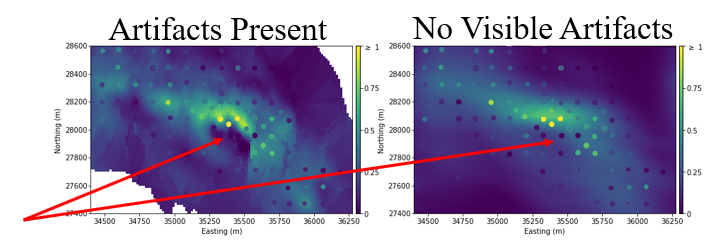
\includegraphics[width=80mm]{./figures/artifacts_example.png}
    \caption{Artifact Example}
    \label{fig:Artifact Example}
\end{figure}

    \subsection{Model Checking Code}\label{model-checking-code}

    \begin{Verbatim}[commandchars=\\\{\}]
{\color{incolor}In [{\color{incolor}33}]:} \PY{n}{Exh\PYZus{}datafl} \PY{o}{=} \PY{n}{gs}\PY{o}{.}\PY{n}{DataFile}\PY{p}{(}\PY{l+s+s1}{\PYZsq{}}\PY{l+s+s1}{sgsim.out}\PY{l+s+s1}{\PYZsq{}}\PY{p}{,}\PY{n}{griddef}\PY{o}{=}\PY{n}{griddef}\PY{p}{)}
         \PY{n}{vlim} \PY{o}{=} \PY{p}{(}\PY{o}{\PYZhy{}}\PY{l+m+mi}{3}\PY{p}{,}\PY{l+m+mi}{3}\PY{p}{)}
         
         \PY{k}{for} \PY{n}{fold} \PY{o+ow}{in} \PY{n+nb}{range}\PY{p}{(}\PY{l+m+mi}{1}\PY{p}{,}\PY{l+m+mi}{6}\PY{p}{)}\PY{p}{:}
             \PY{n}{V\PYZus{}Pred} \PY{o}{=} \PY{n}{gs}\PY{o}{.}\PY{n}{DataFile}\PY{p}{(}\PY{l+s+s1}{\PYZsq{}}\PY{l+s+s1}{./predictions/ensemble\PYZus{}}\PY{l+s+si}{\PYZob{}\PYZcb{}}\PY{l+s+s1}{.dat}\PY{l+s+s1}{\PYZsq{}}\PY{o}{.}\PY{n}{format}\PY{p}{(}\PY{n}{fold}\PY{p}{)}\PY{p}{,}\PY{n}{griddef}\PY{o}{=}\PY{n}{griddef}\PY{p}{)}
             \PY{n}{V\PYZus{}test} \PY{o}{=} \PY{n}{gs}\PY{o}{.}\PY{n}{DataFile}\PY{p}{(}\PY{l+s+s1}{\PYZsq{}}\PY{l+s+s1}{./data/data\PYZus{}test\PYZus{}}\PY{l+s+si}{\PYZob{}\PYZcb{}}\PY{l+s+s1}{.dat}\PY{l+s+s1}{\PYZsq{}}\PY{o}{.}\PY{n}{format}\PY{p}{(}\PY{n}{fold}\PY{p}{)}\PY{p}{,}\PY{n}{griddef}\PY{o}{=}\PY{n}{griddef}\PY{p}{)}
             \PY{n}{V\PYZus{}train} \PY{o}{=} \PY{n}{gs}\PY{o}{.}\PY{n}{DataFile}\PY{p}{(}\PY{l+s+s1}{\PYZsq{}}\PY{l+s+s1}{./data/data\PYZus{}train\PYZus{}}\PY{l+s+si}{\PYZob{}\PYZcb{}}\PY{l+s+s1}{.dat}\PY{l+s+s1}{\PYZsq{}}\PY{o}{.}\PY{n}{format}\PY{p}{(}\PY{n}{fold}\PY{p}{)}\PY{p}{,}\PY{n}{griddef}\PY{o}{=}\PY{n}{griddef}\PY{p}{)}
             \PY{n}{V\PYZus{}test}\PY{o}{.}\PY{n}{data}\PY{p}{[}\PY{l+s+s1}{\PYZsq{}}\PY{l+s+s1}{Z}\PY{l+s+s1}{\PYZsq{}}\PY{p}{]} \PY{o}{=} \PY{l+m+mf}{0.5}
             \PY{n}{idx\PYZus{}test}\PY{p}{,}\PY{n}{ingrid} \PY{o}{=} \PY{n}{griddef}\PY{o}{.}\PY{n}{coord\PYZus{}to\PYZus{}index1d}\PY{p}{(}\PY{n}{x}\PY{o}{=}\PY{n}{V\PYZus{}test}\PY{o}{.}\PY{n}{data}\PY{p}{[}\PY{l+s+s1}{\PYZsq{}}\PY{l+s+s1}{X}\PY{l+s+s1}{\PYZsq{}}\PY{p}{]}\PY{p}{,}\PY{n}{y}\PY{o}{=}\PY{n}{V\PYZus{}test}\PY{o}{.}\PY{n}{data}\PY{p}{[}\PY{l+s+s1}{\PYZsq{}}\PY{l+s+s1}{Y}\PY{l+s+s1}{\PYZsq{}}\PY{p}{]}\PY{p}{,}\PY{n}{z}\PY{o}{=}\PY{n}{V\PYZus{}test}\PY{o}{.}\PY{n}{data}\PY{p}{[}\PY{l+s+s1}{\PYZsq{}}\PY{l+s+s1}{Z}\PY{l+s+s1}{\PYZsq{}}\PY{p}{]}\PY{p}{)}
             \PY{n}{V\PYZus{}test}\PY{o}{.}\PY{n}{data}\PY{p}{[}\PY{l+s+s1}{\PYZsq{}}\PY{l+s+s1}{Z}\PY{l+s+s1}{\PYZsq{}}\PY{p}{]} \PY{o}{=} \PY{l+m+mf}{0.5}
             \PY{n}{idx\PYZus{}train}\PY{p}{,}\PY{n}{ingrid} \PY{o}{=} \PY{n}{griddef}\PY{o}{.}\PY{n}{coord\PYZus{}to\PYZus{}index1d}\PY{p}{(}\PY{n}{x}\PY{o}{=}\PY{n}{V\PYZus{}train}\PY{o}{.}\PY{n}{data}\PY{p}{[}\PY{l+s+s1}{\PYZsq{}}\PY{l+s+s1}{X}\PY{l+s+s1}{\PYZsq{}}\PY{p}{]}\PY{p}{,}\PY{n}{y}\PY{o}{=}\PY{n}{V\PYZus{}train}\PY{o}{.}\PY{n}{data}\PY{p}{[}\PY{l+s+s1}{\PYZsq{}}\PY{l+s+s1}{Y}\PY{l+s+s1}{\PYZsq{}}\PY{p}{]}\PY{p}{,}\PY{n}{z}\PY{o}{=}\PY{n}{V\PYZus{}train}\PY{o}{.}\PY{n}{data}\PY{p}{[}\PY{l+s+s1}{\PYZsq{}}\PY{l+s+s1}{Z}\PY{l+s+s1}{\PYZsq{}}\PY{p}{]}\PY{p}{)}
             \PY{n}{gridsize} \PY{o}{=} \PY{p}{(}\PY{l+m+mi}{3}\PY{p}{,}\PY{l+m+mi}{3}\PY{p}{)}
             \PY{n}{fig} \PY{o}{=} \PY{n}{plt}\PY{o}{.}\PY{n}{figure}\PY{p}{(}\PY{n}{figsize}\PY{o}{=}\PY{p}{(}\PY{l+m+mi}{20}\PY{p}{,} \PY{l+m+mi}{20}\PY{p}{)}\PY{p}{)}
             \PY{n}{ax1} \PY{o}{=} \PY{n}{plt}\PY{o}{.}\PY{n}{subplot2grid}\PY{p}{(}\PY{n}{gridsize}\PY{p}{,}\PY{p}{(}\PY{l+m+mi}{0}\PY{p}{,}\PY{l+m+mi}{0}\PY{p}{)}\PY{p}{)} 
             \PY{n}{ax2} \PY{o}{=} \PY{n}{plt}\PY{o}{.}\PY{n}{subplot2grid}\PY{p}{(}\PY{n}{gridsize}\PY{p}{,}\PY{p}{(}\PY{l+m+mi}{0}\PY{p}{,}\PY{l+m+mi}{1}\PY{p}{)}\PY{p}{)}
             \PY{n}{ax3} \PY{o}{=} \PY{n}{plt}\PY{o}{.}\PY{n}{subplot2grid}\PY{p}{(}\PY{n}{gridsize}\PY{p}{,}\PY{p}{(}\PY{l+m+mi}{0}\PY{p}{,}\PY{l+m+mi}{2}\PY{p}{)}\PY{p}{)}
             \PY{n}{ax4} \PY{o}{=} \PY{n}{plt}\PY{o}{.}\PY{n}{subplot2grid}\PY{p}{(}\PY{n}{gridsize}\PY{p}{,}\PY{p}{(}\PY{l+m+mi}{1}\PY{p}{,}\PY{l+m+mi}{0}\PY{p}{)}\PY{p}{)}
             \PY{n}{ax5} \PY{o}{=} \PY{n}{plt}\PY{o}{.}\PY{n}{subplot2grid}\PY{p}{(}\PY{n}{gridsize}\PY{p}{,}\PY{p}{(}\PY{l+m+mi}{1}\PY{p}{,}\PY{l+m+mi}{1}\PY{p}{)}\PY{p}{)}
             \PY{n}{ax6} \PY{o}{=} \PY{n}{plt}\PY{o}{.}\PY{n}{subplot2grid}\PY{p}{(}\PY{n}{gridsize}\PY{p}{,}\PY{p}{(}\PY{l+m+mi}{1}\PY{p}{,}\PY{l+m+mi}{2}\PY{p}{)}\PY{p}{)}
             \PY{n}{ax7} \PY{o}{=} \PY{n}{plt}\PY{o}{.}\PY{n}{subplot2grid}\PY{p}{(}\PY{n}{gridsize}\PY{p}{,}\PY{p}{(}\PY{l+m+mi}{2}\PY{p}{,}\PY{l+m+mi}{0}\PY{p}{)}\PY{p}{,} \PY{n}{colspan} \PY{o}{=} \PY{l+m+mi}{3}\PY{p}{,}\PY{n}{rowspan} \PY{o}{=} \PY{l+m+mi}{1}\PY{p}{)}
             
             \PY{n}{gs}\PY{o}{.}\PY{n}{pixelplt}\PY{p}{(}\PY{n}{Exh\PYZus{}datafl}\PY{p}{,} \PY{n}{var} \PY{o}{=}\PY{l+s+s1}{\PYZsq{}}\PY{l+s+s1}{value}\PY{l+s+s1}{\PYZsq{}}\PY{p}{,}\PY{n}{griddef}\PY{o}{=}\PY{n}{griddef}\PY{p}{,}\PY{n}{vlim}\PY{o}{=}\PY{n}{vlim}\PY{p}{,} \PY{n}{ax}\PY{o}{=}\PY{n}{ax1}\PY{p}{,}\PY{n}{title} \PY{o}{=} \PY{l+s+s1}{\PYZsq{}}\PY{l+s+s1}{value Truth fold }\PY{l+s+si}{\PYZob{}\PYZcb{}}\PY{l+s+s1}{\PYZsq{}}\PY{o}{.}\PY{n}{format}\PY{p}{(}\PY{n}{fold}\PY{p}{)}\PY{p}{)}                       
             \PY{n}{gs}\PY{o}{.}\PY{n}{pixelplt}\PY{p}{(}\PY{n}{V\PYZus{}Pred}\PY{o}{.}\PY{n}{data}\PY{p}{[}\PY{l+s+s1}{\PYZsq{}}\PY{l+s+s1}{0}\PY{l+s+s1}{\PYZsq{}}\PY{p}{]}\PY{p}{,}\PY{n}{griddef}\PY{o}{=}\PY{n}{griddef}\PY{p}{,}\PY{n}{vlim}\PY{o}{=}\PY{n}{vlim}\PY{p}{,} \PY{n}{ax}\PY{o}{=}\PY{n}{ax2}\PY{p}{,}\PY{n}{title} \PY{o}{=} \PY{l+s+s1}{\PYZsq{}}\PY{l+s+s1}{value ML Prediction fold }\PY{l+s+si}{\PYZob{}\PYZcb{}}\PY{l+s+s1}{\PYZsq{}}\PY{o}{.}\PY{n}{format}\PY{p}{(}\PY{n}{fold}\PY{p}{)}\PY{p}{)}
             \PY{n}{gs}\PY{o}{.}\PY{n}{pixelplt}\PY{p}{(}\PY{p}{(}\PY{n}{V\PYZus{}Pred}\PY{o}{.}\PY{n}{data}\PY{p}{[}\PY{l+s+s1}{\PYZsq{}}\PY{l+s+s1}{0}\PY{l+s+s1}{\PYZsq{}}\PY{p}{]}\PY{o}{\PYZhy{}}\PY{n}{Exh\PYZus{}datafl}\PY{o}{.}\PY{n}{data}\PY{p}{[}\PY{l+s+s1}{\PYZsq{}}\PY{l+s+s1}{value}\PY{l+s+s1}{\PYZsq{}}\PY{p}{]}\PY{p}{)}\PY{p}{,}\PY{n}{griddef}\PY{o}{=}\PY{n}{griddef}\PY{p}{,}\PY{n}{vlim}\PY{o}{=}\PY{p}{(}\PY{o}{\PYZhy{}}\PY{l+m+mi}{1}\PY{p}{,}\PY{l+m+mi}{1}\PY{p}{)}\PY{p}{,} \PY{n}{ax}\PY{o}{=}\PY{n}{ax3}\PY{p}{,}\PY{n}{cmap}\PY{o}{=}\PY{l+s+s1}{\PYZsq{}}\PY{l+s+s1}{bwr}\PY{l+s+s1}{\PYZsq{}}\PY{p}{,}\PY{n}{title}\PY{o}{=}\PY{l+s+s1}{\PYZsq{}}\PY{l+s+s1}{Difference fold }\PY{l+s+si}{\PYZob{}\PYZcb{}}\PY{l+s+s1}{\PYZsq{}}\PY{o}{.}\PY{n}{format}\PY{p}{(}\PY{n}{fold}\PY{p}{)}\PY{p}{)}
             \PY{n}{gs}\PY{o}{.}\PY{n}{scatxval}\PY{p}{(}\PY{n}{V\PYZus{}Pred}\PY{o}{.}\PY{n}{data}\PY{p}{[}\PY{l+s+s1}{\PYZsq{}}\PY{l+s+s1}{0}\PY{l+s+s1}{\PYZsq{}}\PY{p}{]}\PY{p}{[}\PY{n}{idx\PYZus{}test}\PY{p}{]}\PY{p}{,}\PY{n}{V\PYZus{}test}\PY{o}{.}\PY{n}{data}\PY{p}{[}\PY{l+s+s1}{\PYZsq{}}\PY{l+s+s1}{value}\PY{l+s+s1}{\PYZsq{}}\PY{p}{]}\PY{p}{,} \PY{n}{ax}\PY{o}{=}\PY{n}{ax4}\PY{p}{,}\PY{n}{title} \PY{o}{=} \PY{l+s+s1}{\PYZsq{}}\PY{l+s+s1}{Scatterplot Between Estimate And Test Set fold }\PY{l+s+si}{\PYZob{}\PYZcb{}}\PY{l+s+s1}{\PYZsq{}}\PY{o}{.}\PY{n}{format}\PY{p}{(}\PY{n}{fold}\PY{p}{)}\PY{p}{)}
             \PY{n}{gs}\PY{o}{.}\PY{n}{scatxval}\PY{p}{(}\PY{n}{V\PYZus{}Pred}\PY{o}{.}\PY{n}{data}\PY{p}{[}\PY{l+s+s1}{\PYZsq{}}\PY{l+s+s1}{0}\PY{l+s+s1}{\PYZsq{}}\PY{p}{]}\PY{p}{[}\PY{n}{idx\PYZus{}train}\PY{p}{]}\PY{p}{,}\PY{n}{V\PYZus{}train}\PY{o}{.}\PY{n}{data}\PY{p}{[}\PY{l+s+s1}{\PYZsq{}}\PY{l+s+s1}{value}\PY{l+s+s1}{\PYZsq{}}\PY{p}{]}\PY{p}{,} \PY{n}{ax}\PY{o}{=}\PY{n}{ax5}\PY{p}{,}\PY{n}{title} \PY{o}{=} \PY{l+s+s1}{\PYZsq{}}\PY{l+s+s1}{Scatterplot Between Estimate And Train Set fold }\PY{l+s+si}{\PYZob{}\PYZcb{}}\PY{l+s+s1}{\PYZsq{}}\PY{o}{.}\PY{n}{format}\PY{p}{(}\PY{n}{fold}\PY{p}{)}\PY{p}{)}
             \PY{n}{gs}\PY{o}{.}\PY{n}{scatxval}\PY{p}{(}\PY{n}{V\PYZus{}Pred}\PY{o}{.}\PY{n}{data}\PY{p}{[}\PY{l+s+s1}{\PYZsq{}}\PY{l+s+s1}{0}\PY{l+s+s1}{\PYZsq{}}\PY{p}{]}\PY{p}{,}\PY{n}{Exh\PYZus{}datafl}\PY{o}{.}\PY{n}{data}\PY{p}{[}\PY{l+s+s1}{\PYZsq{}}\PY{l+s+s1}{value}\PY{l+s+s1}{\PYZsq{}}\PY{p}{]}\PY{p}{,} \PY{n}{ax}\PY{o}{=}\PY{n}{ax6}\PY{p}{,}\PY{n}{title} \PY{o}{=} \PY{l+s+s1}{\PYZsq{}}\PY{l+s+s1}{Scatterplot Between Estimate And Truth fold }\PY{l+s+si}{\PYZob{}\PYZcb{}}\PY{l+s+s1}{\PYZsq{}}\PY{o}{.}\PY{n}{format}\PY{p}{(}\PY{n}{fold}\PY{p}{)}\PY{p}{)}
             \PY{n}{gs}\PY{o}{.}\PY{n}{histpltsim}\PY{p}{(}\PY{n}{V\PYZus{}Pred}\PY{o}{.}\PY{n}{data}\PY{p}{[}\PY{l+s+s1}{\PYZsq{}}\PY{l+s+s1}{0}\PY{l+s+s1}{\PYZsq{}}\PY{p}{]}\PY{p}{,}\PY{n}{Exh\PYZus{}datafl}\PY{o}{.}\PY{n}{data}\PY{p}{[}\PY{l+s+s1}{\PYZsq{}}\PY{l+s+s1}{value}\PY{l+s+s1}{\PYZsq{}}\PY{p}{]}\PY{p}{,}\PY{n}{griddef}\PY{o}{=}\PY{n}{griddef}\PY{p}{,}\PY{n}{nreal}\PY{o}{=}\PY{l+m+mi}{1}\PY{p}{,} \PY{n}{ax}\PY{o}{=} \PY{n}{ax7}\PY{p}{,}\PY{n}{lw}\PY{o}{=}\PY{l+m+mi}{5}\PY{p}{,} \PY{n}{title} \PY{o}{=} \PY{l+s+s1}{\PYZsq{}}\PY{l+s+s1}{Histogram Reproduction fold }\PY{l+s+si}{\PYZob{}\PYZcb{}}\PY{l+s+s1}{\PYZsq{}}\PY{o}{.}\PY{n}{format}\PY{p}{(}\PY{n}{fold}\PY{p}{)}\PY{p}{)}
             \PY{n}{plt}\PY{o}{.}\PY{n}{tight\PYZus{}layout}\PY{p}{(}\PY{p}{)}
             \PY{n+nb}{print}\PY{p}{(}\PY{l+s+s1}{\PYZsq{}}\PY{l+s+s1}{THe R\PYZhy{}sqaured of fold }\PY{l+s+si}{\PYZob{}\PYZcb{}}\PY{l+s+s1}{ is }\PY{l+s+si}{\PYZob{}\PYZcb{}}\PY{l+s+s1}{\PYZsq{}}\PY{o}{.}\PY{n}{format}\PY{p}{(}\PY{n}{fold}\PY{p}{,}\PY{n}{r2\PYZus{}score}\PY{p}{(}\PY{n}{Exh\PYZus{}datafl}\PY{o}{.}\PY{n}{data}\PY{p}{[}\PY{l+s+s1}{\PYZsq{}}\PY{l+s+s1}{value}\PY{l+s+s1}{\PYZsq{}}\PY{p}{]}\PY{p}{,}\PY{n}{V\PYZus{}Pred}\PY{o}{.}\PY{n}{data}\PY{p}{[}\PY{l+s+s1}{\PYZsq{}}\PY{l+s+s1}{0}\PY{l+s+s1}{\PYZsq{}}\PY{p}{]}\PY{p}{)}\PY{p}{)}\PY{p}{)}
\end{Verbatim}


    \begin{Verbatim}[commandchars=\\\{\}]
THe R-sqaured of fold 1 is 0.7755018251952328
THe R-sqaured of fold 2 is 0.8186455312571943
THe R-sqaured of fold 3 is 0.8982066184090909
THe R-sqaured of fold 4 is 0.8739642470522466
THe R-sqaured of fold 5 is 0.8979186035217999

    \end{Verbatim}

    \begin{center}
    \adjustimage{max size={0.9\linewidth}{0.9\paperheight}}{output_69_1.png}
    \end{center}
    { \hspace*{\fill} \\}
    
    \begin{center}
    \adjustimage{max size={0.9\linewidth}{0.9\paperheight}}{output_69_2.png}
    \end{center}
    { \hspace*{\fill} \\}
    
    \begin{center}
    \adjustimage{max size={0.9\linewidth}{0.9\paperheight}}{output_69_3.png}
    \end{center}
    { \hspace*{\fill} \\}
    
    \begin{center}
    \adjustimage{max size={0.9\linewidth}{0.9\paperheight}}{output_69_4.png}
    \end{center}
    { \hspace*{\fill} \\}
    
    \begin{center}
    \adjustimage{max size={0.9\linewidth}{0.9\paperheight}}{output_69_5.png}
    \end{center}
    { \hspace*{\fill} \\}
    

    % Add a bibliography block to the postdoc
    
    
    
    \end{document}
